\documentclass[draftspec]{sbmlpkgspec}
\usepackage{microtype}
\usepackage{color}
\usepackage[]{todonotes} % preface with "disable" to hide todo notes

%% ============================================================================
%% Description:  Documentation for sbmlpkgspec.cls
%% First author: Michael Hucka <mhucka@caltech.edu>
%% Organization: California Institute of Technology
%% Date created: September 2011
%% https://sbml.svn.sourceforge.net/svnroot/sbml/trunk/project/tex/sbmlpkgspec
%%
%% Copyright (C) 2011-2012 California Institute of Technology, Pasadena, CA.
%%
%% SBMLPkgSpec is free software; you can redistribute it and/or modify it
%% under the terms of the GNU Lesser General Public License as published by
%% the Free Software Foundation.  A copy of the license agreement is provided
%% in the file named "LICENSE.txt" included with this software distribution.
%% ============================================================================

% Macros just for this document:

\newcommand{\sbmlpkg}{\texorpdfstring{%
    \textls[-25]{\textsc{SBMLPkgSpec}}}{%
    \textsc{SBMLPkgSpec}}\xspace}
\newcommand{\sbmlpkghead}{\texorpdfstring{%
    \textls[-50]{\textsc{SBMLPkgSpec}}}{%
    \textsc{SBMLPkgSpec}}\xspace}
\newcommand{\sbmlpkgfile}{\literalFont{sbmlpkgspec.cls}\xspace}
\newcommand{\latex}{\LaTeX{}\xspace}
\newcommand{\tex}{\TeX{}\xspace}
\newcommand{\distURL}{http://sourceforge.net/projects/sbml/files/specifications/tex}
\newcommand{\srcURL}{https://sbml.svn.sourceforge.net/svnroot/sbml/trunk/project/tex/sbmlpkgspec}
\newcommand{\webURL}{http://sbml.org/Documents/Specifications/The_SBMLPkgSpec_LaTeX_class}
\newcommand{\cmd}[1]{\literalFont{\textbackslash #1}}

% Custom latex listing style, for use with the listings package.  The default
% highlights far too many things, IMHO.  This keeps it simple and only adjusts
% the appearance of comments within listings.

\lstdefinelanguage{mylatex}{%
  morekeywords={},%
  sensitive,%
  alsoother={0123456789$_},%$
  morecomment=[l]\%%
}[keywords,tex,comments]

\lstdefinestyle{latex}{language=mylatex}


%Listing style for SBOL RDF/XML serialization examples
\usepackage{listings}
\usepackage{color}
\usepackage{xcolor} 
\definecolor{dkgreen}{rgb}{0,0.6,0}
\definecolor{gray}{rgb}{0.5,0.5,0.5}
\definecolor{light-gray}{gray}{0.97}
\lstdefinelanguage{sbol}
    {morekeywords={xmlns:sbol,rdf:about,sbol:displayId,sbol:persistentIdentity,sbol:version,sbol:timeStamp,sbol:name,sbol:description,sbol:member,sbol:Collection,sbol:type, sbol:role, sbol:ComponentDefinition, sbol:MapsTo, sbol:sequence,sbol:wasDerivedFrom,sbol:Component,sbol:subComponent,sbol:SequenceAnnotation,sbol:component,sbol:location, sbol:sequenceAnnotation, sbol:Range, sbol:start, sbol:end, sbol:orientation,sbol:SequenceConstraint, sbol:restriction, sbol:subject, sbol:object,sbol:Sequence, sbol:elements, sbol:encoding,sbol:Model, sbol:source, sbol:language, sbol:framework,sbol:FunctionalComponent, sbol:Module, sbol:Interaction, sbol:interaction, sbol:module, sbol:model,sbol:Model,sbol:definition, sbol:access, sbol:direction, sbol:mapsTo, sbol:refinement, sbol:local, sbol:remote, sbol:participation, sbol:Participation, sbol:participant,sbol:sequenceConstraint,sbol:at,sbol:Cut,sbol:functionalComponent,sbol:ModuleDefinition},
     basicstyle=\fontsize{7}{9}\selectfont\ttfamily,
     backgroundcolor=\color{light-gray},
     keywordstyle=\color{blue},
     commentstyle=\color{gray},
     stringstyle=\color{dkgreen},
     tabsize=2,
     showspaces=false,
     showstringspaces=false,
     breaklines=true,                           % wrap text
     sensitive=true,                            % keywords are case sensitive
     %morecomment=[l][commentstyle]{\#},         % comment format
     morestring=[b]",                           % string format
     escapeinside={[}{]},
     alsoletter=:
     %breakatwhitespace=true, 
     %literate={\-}{}{0\discretionary{a}{\\}{}}
}

%Command to format the listings containing SBOL RDF/XML serialization examples
\newcommand{\lstsetsbol}{
 \lstset{language=sbol,
        tabsize=2
 }
}

%Commands to format SBOL terms in the document
\newcommand{\sbolheading}[1]{\texttt{#1}}
\newcommand{\sbol}[1]{\texttt{\hyperref[sec:#1]{#1}}}
\newcommand{\refObj}[1]{$\langle$#1$\rangle$}
% Decision vs. Low-Priority Decision vs. Clarification TODOs:
\newcommand{\Dtodo}[1]{\todo[inline,color=red]{#1}}
\newcommand{\LDtodo}[1]{\todo[inline,color=yellow]{#1}}
\newcommand{\Ctodo}[1]{\todo[inline,color=cyan]{#1}}
% Resolved but still awaiting review:
\newcommand{\Rtodo}[1]{\todo[inline,color=green]{#1}}
% Deferred to the next (minor) version
\newcommand{\NVtodo}[1]{\todo[inline,color=blue]{#1}}

%Command to format external terms in the document
\newcommand{\external}[1]{\texttt{#1}}


% -----------------------------------------------------------------------------
% Start of document
% -----------------------------------------------------------------------------

\begin{document}

\packageTitle{\latex Class for SBML Package Specifications}
\packageVersion{Version 2.0.0}
\packageVersionDate{24 April 2015}

\title{BBF RFC ?: Synthetic Biology Open Language \texorpdfstring{\\[3pt]}{}\mbox{(SBOL) Version~2.0.0}}


\author{Nicholas Roehner\\[0.25em]
\mailto{nicholasroehner@gmail.com}\\[0.25em]
  Electrical and Computer Engineering\\
  Boston University\\
  Boston, MA, USA\\
  \\
  Matthew Pocock\\
\mailto{turingatemyhamster@gmail.com}\\
  Turing Ate My Hamster LTD\\
  7 Station RD, Backworth, NE27 0RT
}


\author{\begin{tabular}{l>{\hspace*{15pt}}r}
Bryan Bartley		& \emph{University of Washington, US}\\
Jacob Beal			& \emph{Raytheon BBN Technologies, US}\\
Kevin Clancy		& \emph{ThermoFischer Scientific, US}\\
Goksel Misirli		& \emph{Newcastle University, GB}\\
Nicholas Roehner	& \emph{Boston University, US}\\
Matthew Pocock  	& \emph{Newcastle University, GB}\\
Curtis Madsen		& \emph{Newcastle University, GB}\\
lots of other community members & all over the world\\
Chris Myers			& \emph{University of Utah, US}\\
Anil Wipat			& \emph{Newcastle University, GB}\\
Herbert Sauro		& \emph{University of Washington, US}\\[8pt]
\end{tabular}\\
\href{mailto:editors@sbolstandard.org}{\sffamily editors@sbolstandard.org}
\LDtodo{What should be the authorship? -JSB}}



\maketitlepage
\maketableofcontents

\Rtodo{When editing, change the todos that you handle to ``Rtodo'' (``R'' for ``resolved''), rather than just deleting them, so that a second person can review}

\Ctodo{Final pass before release must include:

Ensure that all references are defined precisely once (grep 'undefined' and 'multiply' in log)

Make sure all requirements words are properly upper-cased

Spell check

Ensure that TOC links to correct locations}


% -----------------------------------------------------------------------------
\section{Purpose}
% -----------------------------------------------------------------------------
% Synthetic biology aims to apply engineering principles such as standardization, modularity, and design abstraction to molecular biology.  However, synthetic biology still faces substantial challenges, including long development times, high rates of failure, and poor reproducibility. 

% The Synthetic Biology Open Language is intended to help synthetic biologists collaborate by allowing them to exchange designs in a standardized data format.  In addition, the SBOL data model systematically describes the essential details of a design that are required for researchers to reproduce each other's designs in the laboratory.  The purpose of the Synthetic Biology Open Language is to aid collaboration between researchers, improve scientific reproducibility, and to speed the research and development of technologies based on synthetic biology.

Synthetic biology builds upon the techniques and successes of genetics, molecular biology, and metabolic engineering by applying engineering principles to the design of biological systems. These principles include standardization, modularity, and design abstraction. The field still faces substantial challenges, including long development times, high rates of failure, and poor reproducibility. A common factor of these challenges is the exchange of information about designed systems between laboratories. 
When designing a synthetic system,  synthetic biologists need to exchange information about multiple types of molecules and their expected behavior in the design.
Moreover, there is often one or more steps of separation between a specified nucleic acid sequence (e.g., the sequence that encodes an enzyme or transcription factor) and the interactions that are being reasoned about in order to determine that sequence (e.g., chemical modification of metabolites or regulation of gene expression), yet these different perspectives are often intimately tied together in the engineering of biological systems.

The \emph{Synthetic Biology Open Language} has been designed as a standard to support the specification and exchange of such information in synthetic biology, filling a need not satisfied by other pre-existing standards.
Previous nucleic acid sequence description formats lack key capabilities: simple sequence encoding formats such as FASTA encode almost nothing about design rationale, while more sophisticated formats such as GenBank and Swiss-Prot support a flat annotation of sequence features that is well suited for description of natural systems but unable to represent either the multi-layered design structure common to engineered systems or the functional roles or consequences of these sequences.
\ref{f:sequence} shows the relationship of selected prior sequence description formats to SBOL 1.1 and SBOL 2.0.
Modelling languages, such as the Systems Biology Markup Language (SBML) ~\cite{SBML} can be used represent biological processes, but is not sufficient to represent the associated nucleotide or amino acid sequences.  %Goksel: Commented this sentence: Kinetic information may be present in SBML~\cite{SBML} or mass conservation laws in other systems such as the COBRA Toolbox~\cite{COBRA}. 
Synthetic biology needs a structured standard with defined ways on how to represent relevant molecules and their functional roles within the designed system, standardized rules on how such information is encoded in the file and the means to enable exchange of such data between participating laboratories as part of publications. 
%Goksel: Updated the sentence as above:Systems Biology Markup Language (SBML) represents reactions, pathways, and models, but does not typically represent the associated sequences.

To help address these challenges, the SBOL introduces a standardized format for the electronic exchange of information describing the structural and functional aspects of biological designs. 
The standard is designed to support the development of explicit and unambiguous data models of biological designs through the use of a well defined data model on how to represent the biological molecules, and their structural and functional roles in a systematic fashion. 
The standard further describes rules and best practices on how to include, develop, and populate this format with relevant information of essential design details. 
SBOL uses existing Semantic Web resources such as biological ontologies and \emph{Universal Resource Identifiers} (URIs) to unambiguously define genetic design elements.
%Anil: I think we need to say just a bit more here about how we support extensions to the core data model using annotations. I think the sentences removed below were hinting at that. 
%Goksel: Replaced thi sentence with the one above:Because the standard itself can represent information from other sources for sequence representations, reaction information and ontologies to represent biological design information, the standard uses modern information exchange techniques such as \emph{Universal Resource Identifiers} (URIs). This permits the reuse of existing information without the need to repeat it, thus avoiding both redundancy and likely future information decay within shared files. 
%Goksel: Removed this sentence: The ultimate utility of URIs in the SBOL standard is the ability to support flexible annotation with appropriate metadata while associating an authority with that annotation. 
The definition of the data model and associated format, the rules on the addition of data within the format and the representation of this in electronic data files are intended to make the SBOL standard a useful means of promoting global data exchange between laboratories and between software programs.

This document presents the second version of SBOL.
The previous version 1.1 of the SBOL standard focused on representing the structural aspects of genetic designs. 
Users of the standard were able to use it to exchange information on DNA designs but could not represent molecules other than DNA or represent the functional aspects of their designs beyond the DNA sequences. 
To serve as an effective medium for the computational exchange of genetic designs, SBOL must be extended to capture more aspects of a designed system, including both structural and functional information, and the composition of complex structural and functional designs by combining simpler parts. 
The SBOL 2.0 data model defined in this specification thus extends the prior model to provide for addressing the most pressing needs for expanding SBOL version 1.1, in particular it can:
\begin{itemize}

\item represent structural components of a biological design, including DNA, RNA, proteins, small molecules and other physical components

\item describe behavioral aspects of a biological design, the intended or expected interactions and dynamic behavior

\item associate structure and function together, so that a single design can be understood both in terms of its structure and its behavior

\item support rich annotations of all components, so that data required to describe a design, but not formalized in this specification can be safely exchanged

\end{itemize}
Taken together, these capabilities allow SBOL sufficient expressiveness to support the description and exchange of hierarchical, modular representations of both the intended structure and function of designed biological systems.

\begin{figure}
\centering
\includegraphics[width=5in]{images/format-comparison.pdf}
\caption{SBOL 2.0 extends prior sequence description formats to represent both structure and function of a genetic design in a single model.}
\label{f:sequence}
\end{figure}

To address the need for functional descriptions in SBOL, the proposed data model adds new classes to provide a firm basis for functional representation in SBOL without going so far as to create a new standard for mathematically modeling biology, as there already exist several established languages for doing so, from the SBML to CellML~\cite{CellML} and even MatLab~\cite{matlab}. Rather, these classes enable users of SBOL to group components that function together, describe the basic qualitative interactions between these components, and document references to standard mathematical models that are external to SBOL and that provide more detailed descriptions of component function. In other words, a module definition gathers together a set of component instantiations, a set of interactions between these component instantiations, and a set of references to external models that are expected to be consistent with the module's interactions.

The SBOL 2.0 specification also adds a number of measures to simplify adoption and validation of compatibility with the standard.
First, the specification explicitly incorporates its serialization format into the specification, whereas SBOL 1.1 used an implicit standard tied to a reference implementation.
Second, the specification includes a set of validation rules for determining compatibility of a document with SBOL 2.0, most of which are machine-verifiable.
Finally, the specification includes a set of recommended best-practices likely to allow a tool to take best advantage of the standard and other compatible tools.

Care has been taken to ensure that SBOL 2.0 is backward-compatible with SBOL 1.x.  
The generalization of the data model does mean that many names have changed and thus an SBOL 1.x file is not a valid SBOL 2.0 file.
There is, however, a direct mapping from the SBOL 1.x data model into the SBOL 2.0 data model, making it simple to automatically ``upgrade'' any SBOL 1.x file into and SBOL 2.0 file.
% Goksel - Removed this sentence:Therefore, SBOL 2.0 supersedes SBOL 1.1, and developers are encouraged to use it for all new software efforts.  
Since SBOL 2.0 can encode all data previously encoded in SBOL 1.1, developers are also encouraged to upgrade their SBOL 1.1 compliant software tools to use SBOL 2.0 data objects. 

As discussed previously, SBOL 2.0 allows designs to be described beyond the simple annotated DNA sequence offered in SBOL 1.1. Of equal importance in SBOL 2.0 is the explicit provision of mechanisms that allows SBOL to be easily extended~\cite{sec:Annotation}. The intent of SBOL is to allow designs of synthetic biological systems to be fully described so that such designs can be reproduced. However SBOL does not currently offer a full catalog of data %Note I'm using data not metadata to avoid technical terms at this state
to allow one to achieve complete reproducibility. For example the proposed standard does not yet include environmental and host context information or details on how the performance of the design is measured. Such details can now be included in SBOL through an explicit extension mechanism. Three scenarios are envisaged for extending SBOL:

\begin{itemize}
\item Use of the extension mechanism to include critical information related to the reproducibility of designs. For example, what growth media was used, what temperature were the organisms grown at, when were they harvested, was the DNA integrated into the host genome (if so here), or in a plasmid (what plasmid).
\item For tool makers, the extension mechanism allows tool specific information to be added to SBOL. Such information could include tool settings specific to the design that is being loaded, for example what windows should be opened or settings initialized. Tool makers could also include encrypted proprietary information related to the company or client in an extension. 
\item Non-essential information to reproducibility but nevertheless useful information for many users. There are many cases where a community of users require specific information not available in core of SBOL. Examples include visualization information, how the DNA was assembled, information on evolutionary stability, or specialist modeling information.
\end{itemize}

The extension mechanism is therefore a critical part of SBOL 2.0 and will allow others in the community to incoroporate either their own requirements for data into SBOL or contribute to community efforts to expand the scope of SBOL.


The SBOL standard has been developed in collaboration between both ``wet'' bench scientists and ``dry'' scientific modelers and tool designers active within the synthetic biology community. 
As with the earlier SBOL 1.1 standard, this community (open for any practitioner to join) has met to discuss, argue and agree upon needs that the SBOL standard should address. 
This information has then been used by developers within our community to design, develop, and test a specification of the standard. The specification has been tested by the community through several iterations for the ability to represent a wide range of synthetic biology design projects, as well as, the ability to share designs between different laboratories. 
The standard has also been used to develop software tools that employ the standard for developing and sharing synthetic design projects. 
The publication of this specification is intended to make these capabilities more widely accessible to the community of potential developers and users.

% -----------------------------------------------------------------------------
%\section{Relation to other BBF RFCs}
% -----------------------------------------------------------------------------

% -----------------------------------------------------------------------------
\section{Copyright and License Statement}
% -----------------------------------------------------------------------------

%% Variation from BBF RFC 0 specs confirmed in email communication with BBF by Jake Beal, 3/21/15

Copyright (C) The BioBricks Foundation and all authors listed on this BBF RFC. This work is made available under the Creative Commons Attribution 4.0 International Public License. To view a copy of this license visit \href{https://creativecommons.org/licenses/by/4.0/}{https://creativecommons.org/licenses/by/4.0/}.

In addition to the listed authors, the following people are specifically recognized as additional contributors sharing in the copyright (alphabetically by institution):
Douglas Densmore (Boston University, USA), 
Jacqueline Quinn (Google, USA), and
Guy-Bart Stan (Imperial College London, UK).

The authors would also like to thank Michael Hucka for developing the LaTeX style file used to develop this document~\citep{hucka2017sbmlpkgspec}.


% -----------------------------------------------------------------------------
\section{History and Acknowledgements}
% -----------------------------------------------------------------------------
%Add yourself if you have helped and aren't on the list

SBOL originated in discussions between participants in the Synthetic Biology Open Language Workshops held in Blacksburg, Virginia on January 7-10, 2011, and its further development has continued at a series of subsequent open invitation workshops and through email exchanges on the SBOL Developers mailing list. 

Contributors to this work include: Bryan Bartley (University of Washington), Jacob Beal (BBN Technologies), Goksel Misirli (Newcastle University), Chris J. Myers (University of Utah), Matthew Pocock (Newcastle University and Turing Ate My Hamster LTD), Nicholas Roehner (Boston University), Herbert M. Sauro (University of Washington), Anil Wipat (Newcastle University).

\todo[inline]{Get lots more authors to sign on}

\todo[inline]{Make Herbert write something nice about histor to add here -JSB}

% -----------------------------------------------------------------------------
\section{SBOL Specification Vocabulary}
% -----------------------------------------------------------------------------

\subsection{Term Conventions}

This document indicates requirement levels using the controlled vocabulary specified in IETF RFC 2119 and reiterated in BBF RFC 0.
In particular, the key words "MUST", "MUST NOT", "REQUIRED", "SHALL", "SHALL NOT", "SHOULD", "SHOULD NOT", "RECOMMENDED", "MAY", and "OPTIONAL" in this document are to be interpreted as described in RFC 2119.

\begin{itemize}
\item The words "MUST", "REQUIRED", or "SHALL" mean that the item is an absolute requirement.
\item The phrases "MUST NOT" or "SHALL NOT" mean that the item is an absolute prohibition.
\item The word "SHOULD" or the adjective "RECOMMENDED" mean that there may exist valid reasons in particular circumstances to ignore a particular item, but the full implications must be understood and carefully weighed before choosing a different course.
\item The phrases "SHOULD NOT" or "NOT RECOMMENDED" mean that there may exist valid reasons in particular circumstances when the particular behavior is acceptable or even useful, but the full implications should be understood and the case carefully weighed before implementing any behavior described with this label.
\item The word "MAY" or the adjective "OPTIONAL" mean that an item is truly optional.
\end{itemize}

\subsection{SBOL Class Names}

SBOL defines the following ``top-level'' and dependent classes:

\begin{description}

\item \emph{\sbol{Collection}}:
Represents a user-defined container for organizing a group of SBOL objects.

\item \emph{\sbol{ComponentDefinition}}: Describes the structure of designed entities, such as DNA, RNA, and proteins, as well as other entities they interact with, such as small molecules or environmental properties.

\begin{itemize}
\item \emph{\sbol{Component}}:
Pointer class. Incorporates a child \sbol{ComponentDefinition} \textit{by reference} into exactly one parent \sbol{ComponentDefinition}. Represents a specific occurrence or instance of an entity within the design of a more complex entity. Because the same definition may appear in  multiple designs or multiple times in a single design, a single \sbol{ComponentDefinition} may have zero or more parent \sbol{ComponentDefinition}s, and each such parent-child link requires its own, distinct \sbol{Component}.
% Mike Bissell - Clarified the role of this class to match changes below in section six. Introduced the term "pointer class" after consulting briefly with Chris M. The emphasis on pointer classes is on the definitions they point to. WAS: "Represents a specific occurrence or instance of a single entity within the design of a more complex component. Each Component is associated with a ComponentDefinition, and there may be many different instances at different locations in a design that share the same definition." I felt this was necessary because it is too easy for a novice to get confused about Component vs. ComponentDefinition here, where they first encounter Component, even before ComponentDefinition is defined.

\item \emph{\sbol{Location}}:
Specifies the base coordinates and orientation of a genetic feature on a DNA or RNA molecule or a residue or site on another sequential macromolecule such as a protein.

\item \emph{\sbol{SequenceAnnotation}}:
Describes the \sbol{Location} of a notable sub-sequence found within the \sbol{Sequence} of a \sbol{ComponentDefinition}. Optionally links to and effectively positions a child \sbol{Component}.
% Mike Bissell - Reworded for clarity of the relationship between ComponentDefinition and Sequence. Broke the original paragraph into two sentences for simplicity. Reworded second sentence to emphasize that a Component is a) a child entity, and b) a link (pointer). Old wording was vague on Component's job within SequenceAnnotation, and old wording made it sound as if the Component was the payload itself, rather than just a reference. WAS: "Describes the Location of a notable sub-sequence found within the Sequence linked to a ComponentDefinition, with an optional link to a Component."

\item \emph{\sbol{SequenceConstraint}}:
Describes the relative spatial position and orientation of two \sbol{Component} objects that are contained within the same \sbol{ComponentDefinition}.
\end{itemize}

\item \emph{\sbol{GenericTopLevel}}:
Represents a data container that can contain custom data added by user applications.

\item \emph{\sbol{Model}}:
Links to quantitative or qualitative computational models that may be used to predict the functional behavior of a biological design.
%Goksel - Updated as above: Links an SBOL representation of biological components and their interactions to quantitative, computational models that may be used to predict the functional behavior of a biological design.

\item \emph{\sbol{ModuleDefinition}}:
Describes a ``system'' design as a collection of biological components and their functional relationships.

\begin{itemize}
\item \emph{\sbol{FunctionalComponent}}:
Pointer class. Incorporates a child \sbol{ComponentDefinition} \textit{by reference} into exactly one parent \sbol{ModuleDefinition}. Represents a specific occurrence or instance of an entity within the design of a system. Because the same definition may appear in multiple designs or multiple times in a single design, a single \sbol{ComponentDefinition} may have zero or more parent \sbol{ModuleDefinition}s, and each such parent-child link requires its own, distinct \sbol{FunctionalComponent}.
% Mike Bissell - As above, reworded to clarify the structure of these relationships, with special attention to the pointer-like nature of this type. WAS: "Represents a specific occurrence or instance of an ComponentDefinition within a ModuleDefinition. Exactly like a Component, except that it can be associated with information about its context of use in the Module, rather than in the context of a containing ComponentDefinition." I eliminated the bit about it being "exactly like... except," because with those exceptions, the likeness is *inexact*. Instead, I deliberately reworked the paragraph's phrasing and contents to emphasize this class's similarity to the other two pointer classes. I felt this was necessary because it is easy for a novice to get confused about FunctionalComponent vs. Component vs. ComponentDefinition in this context.

\item \emph{\sbol{Interaction}}:
Describes a functional relationship between biological entities, such as regulatory activation or repression, or a biological process such as transcription or translation.

\item \emph{\sbol{MapsTo}}:
When a design (\sbol{ComponentDefinition} or \sbol{ModuleDefinition}) includes another design as a sub-design, the parent design may need to refer to a \sbol{ComponentInstance} (either a \sbol{Component} or \sbol{FunctionalComponent}) in the sub-design.
In this case, a \sbol{MapsTo} needs to be added to the instance for the sub-design, and this \sbol{MapsTo} must link between the \sbol{ComponentInstance} in the sub-design and a \sbol{ComponentInstance} in the parent design.

\item \emph{\sbol{Module}}:
Pointer class. Incorporates a child \sbol{ModuleDefinition} \textit{by reference} into exactly one parent \sbol{ModuleDefinition}. Represents a specific occurrence or instance of a subsystem within the design of a larger system. Because the same definition in multiple designs or multiple times in a single design, a single \sbol{ModuleDefinition} may have zero or more parent \sbol{ModuleDefinition}s, and each such parent-child link requires its own, distinct \sbol{Module}.
% Mike Bissell - Reworked this paragraph like I did for Component and FunctionalComponent (see above). WAS: "Represents a specific occurrence or instance of a sub-system within a larger design. Each Module is associated with a ModuleDefinition, and there may be many different instances at different locations in a design that share the same definition." I felt this was necessary because it is way too easy for a novice to get confused about Module vs. ModuleDefinition in this (introductory) context.

\item \emph{\sbol{Participation}}:
Describes the role that a \sbol{FunctionalComponent} plays in an \sbol{Interaction}.
For example, a transcription factor might participate in an \sbol{Interaction} as a repressor or as an activator.

\end{itemize}

\item \emph{\sbol{Sequence}}:
Generally represents a contiguous series of monomers in a macromolecular polymer such as DNA, RNA, or protein. A \sbol{Sequence} can also encode the atoms and bonds of a molecule with non-linear structure (see \ref{sec:Sequence}).

\end{description}

% % -----------------------------------------------------------------------------
\section{Overview of SBOL}
% % -----------------------------------------------------------------------------

\Rtodo{I took a stab at revising this especially in explaining Figure 2. Needs review.  -CJM}

Synthetic biology designs can be described using:
\begin{itemize}
\item Structural terms, e.g., a set of annotated sequences or information about chemical makeup.
\item Functional terms, e.g., the way that components might interact with each other and the overall behavior.
\end{itemize}
In broad strokes, SBOL 1.1 focuses on physical, structural information, whereas SBOL 2.0 includes functional aspects. The physical information about a designed genetic circuit includes the order of its constituents and their descriptions. The exact locations of these constituents and their sequences allow genetic circuits to be defined unambiguously, and reused in other designs. SBOL 2.0 extends SBOL 1.1 in several ways: it extends physical descriptions to include entities beyond DNA sequences, and it allows for functional descriptions of the design. 

As an example, consider the design of an expression cassette, such as found in the plasmid pUC18 \cite{L08752.1}, a device that is designed to detect successful versus unsuccessful molecular cloning. As an overall system, the device is designed to grow either blue-colored (unsuccessful) or white-colored (successful) colonies in the presence of IPTG and the chemical X-gal. Internally, the device has a number of parts, including a promoter, the lac repressor binding site, and the lacZ coding sequence. These parts have specific component-level interactions with IPTG and X-gal, as well as native host gene products, transcriptional and translational machinery that collectively lead to the desired system-level behavior. 

Understanding how such a device works within the context of a host and how it might be adapted to new experimental applications is currently passed on through working with fellow scientists or reading articles in papers and books. But there is no systematic way of communicating the integration of sequence with functional design, so users typically have to look in many different places to develop an understanding of this system.  
The SBOL standard allows designers to describe these functional characteristics, and to connect them to the physical parts and sequences that make up the design. 

SBOL includes two main classes that match the structural/functional distinction above:
\begin{itemize}
\item The \sbol{ComponentDefinition} object describes the physical aspects of the designed system, such as the DNA or RNA sequences and the physical relationships among sub-components.
\item The \sbol{ModuleDefinition} object describes the local interactions of the designed system, such as specific binding relationships, and repression and activation relationships. 
\end{itemize}

Figure 1 shows a simplified view of these classes, as well as other helper classes in SBOL. To continue with the pUC18 example, the description would begin by creating a top-level \sbol{ModuleDefinition}.  The \sbol{ModuleDefinition} specifies the structural elements that make up the cassette by referencing a number of \sbol{ComponentDefinition} objects. These would include the DNA component for the promoter and the small molecule component for IPTG, for example.  
The \sbol{ComponentDefinition} objects can be organized hierarchically.  For example, the plasmid \sbol{ComponentDefinition} may reference \sbol{ComponentDefinition}s for the promoter, coding sequence, etc.  
Each \sbol{ComponentDefinition} object can also include the actual \sbol{Sequence} information (if available), as well as \sbol{SequenceAnnotation} objects that identify the locations of the promoters, coding sequences, etc., on the \sbol{Sequence}.  
In order to specify functional information, the \sbol{ModuleDefinition} can specify \sbol{Interaction} objects that describe any qualitative relationships among components, such as how IPTG and X-gal interact with the gene projects.  Finally, \sbol{ModuleDefinition} object can point to a \sbol{Model} object that provides a reference to a complete quantitative model using a language such as SBML, CellML, Matlab, etc.  Finally, all the of elements of the genetic design can be grouped together within a \sbol{Collection}.

\begin{figure}[ht]
\begin{center}
\includegraphics[scale=0.7]{images/OverviewFigforSpec-v6.png}
\caption{Main classes of information represented by the SBOL standard, and their relationships.  Red boxes are classes from the SBOL 1.1 that focused on structure, whereas blue classes are some of the new classes that support the functional aspects of designs.}
\label{images:overview1}
\end{center}
\end{figure}

% SBOL aims to facilitate the communication and reuse of synthetic biology designs. Given that these designs leverage biochemical knowledge and that they ultimately affect biological systems, it is important that SBOL interacts well with other relevant standards and resources, such as GenBank \cite{genbank}, SwissProt \cite{swissprot}, SBML \cite{SBML}, ChEBI\cite{chebi}, or the Sequence Ontology \cite{so}. Thus, SBOL leverages semantic web technologies, using RDF as a serialization format, and URIs (\emph{Universal Resource Identifiers}) for its objects. URIs allow for direct and un-ambiguous reuse of designs---if a designer in Newcastle wishes to refer to a particular design built in California, he or she can simply name the URI of the ModuleDefinition that describes that design. 

% In sum, we hope that the SBOL standard will enable sharing of synthetic biology designs across the web, and allow developers to more easily build up rich, complex designs by re-using the work of others. 


% Figure 2 extends this view to provide a more detailed view of these classes. 


% Figure 1 illustrates the relationships between the main classes of information encoded by SBOL.  
% The physical structure of an element is represented with a \sbol{ComponentDefinition}, often corresponding to a particular \sbol{Sequence} (e.g., DNA, RNA, amino acids), and with its structure further described in terms of the smaller \sbol{Component} instances contained within, and their absolute and relative positions within the component.
% Functional relationships are represented with a \sbol{ModuleDefinition}, often also described by some \sbol{Model}, and with its structure further described in terms of the smaller \sbol{Module} instances contained within, as well as particular components (designated \sbol{FunctionalComponent} to indicate their use in defining a module), and their interactions.

Figure~\ref{images:overview2} provides a more detailed view the the class structure for the SBOL 2.0 data model.  The main, or \emph{top level} classes, are \sbol{Collection}, \sbol{ComponentDefinition}, sbol{Sequence}, \sbol{ModuleDefinition}, and \sbol{Model}.  The key distinction of these classes is that they can stand alone and be referenced by other top level objects (see the dashed arrows between the green boxes).  The purpose of these classes is described above.  Each of these classes is assisted in their purpose by several \emph{child} classes.  The key distinction of a child object is that it is owned by its parent object, and if that parent object is removed, so is the child object.  This ownership is indicated using the solid arrows in the figure.  For example, a \sbol{ComponentDefinition} owns its \sbol{SequenceAnnotation}s.  Another important distinction in this diagram are the additional additional \emph{instantiation} classes, \sbol{Component}, \sbol{FunctionalComponent}, and \sbol{Module}.  As described above, a \sbol{ModuleDefinition} may include instantiations of \sbol{ComponentDefinitions}.  These instantiations are called \sbol{FunctionalComponent}s.  Furthermore, \sbol{ModuleDefinition}s and \sbol{ComponentDefinition}s can be constructed hierarchically of instantiations of the same time, and these instantiations are called \sbol{Module}s and \sbol{Component}s, respectively.  Using a software analogy, a \sbol{ComponentDefinition} or \sbol{ModuleDefinition} are a class definition while a \sbol{Component}, \sbol{FunctionalComponent}, or \sbol{Module} are an object of that class type.  Finally, one last thing to notice is that child objects can be referenced.  For example, an \sbol{Interaction} is between \sbol{FunctionalComponent} object(s) referenced through the \sbol{Participation} class.  Since this is only a reference, if an \sbol{Interaction} is removed, its \sbol{Participation} objects would be removed but not the \sbol{FunctionalComponent}s that they refer to.  Similarly, \sbol{SequenceAnnotation}s and \sbol{SequenceConstraint}s (provide relative positioning information) only refer to the \sbol{Component}s that they provide positioning information for.


\begin{figure}[ht]
\begin{center}
\includegraphics[scale=0.7]{images/OverviewFig2-v3.png}
\caption{Main classes of information represented by the SBOL standard, and their relationships.  Green boxes are ``top level'' classes, while the other classes are in support of these classes. Solid arrows indicates "contains", whereas a dashed arrow indicates that one class refers to an object of another class.}
\label{images:overview2}
\end{center}
\end{figure}

% The \sbol{Sequence} is a fundamental information object for synthetic biology and is needed to reuse components, to replicate synthetic biology work, and to assemble new synthetic biological systems. In designed systems such objects can consist of small chemical molecules, DNAs, RNAs or Proteins. The \sbol{Sequence} object has been designed to encapsulate any of these types of molecules. Small molecule \sbol{Sequence} objects are typically referred to via their chemical formulae. Molecules where sequence specific information is important, such as DNA, RNA and Protein \sbol{Sequence} objects, use the object to incorporate this information. The \sbol{Sequence} object encapsulates this positional information as well as the associated experimental work or other information related to a sequenced molecule.

% \Rtodo{need to make it clear that it includes DNA, RNA, and protein, also smooth the text --JSB made addiitons based upon the suggested changes - KC}

% In the SBOL data model, a structural layer defines the physical arrangement of components in a biological system.  \sbol{ComponentDefinition}s define genetic elements such as promoters, RBSs, CDSs, and terminators, as well as RNA, proteins, and small molecules.  In a structural hierarchy, \sbol{ComponentDefinition}s can contain subcomponents (\sbol{Component}s), which are instances of the \sbol{ComponentDefinition} for that subcomponent.  A functional layer can be defined to describe the behaviors that arise from the structural layer.  \sbol{ModuleDefinition}s contain information about molecular interactions and their participating components.  They can contain \sbol{FunctionalComponent}s that are instances of \sbol{ComponentDefinition}s that can be assigned functional properties, and they can also contain other modules in a functional hierarchy.  The functions and interactions of these components and other modules within the \sbol{ModuleDefinition} can be quantitatively or qualitatively described using a \sbol{Model}. The \sbol{SequenceAnnotation} object defines data associated the \sbol{Sequence} and \sbol{ComponentDefinition} objects that is needed beyond basic definitions. This can refer to local annotations of the object as well as a container for URIs to external information sources. 


% SBOL includes different entities to describe such genetic circuits. Genetic elements such as a promoter, ribosome binding site (RBS), coding sequence (CDS), or terminator are defined with the \sbol{ComponentDefinition} entity. Their instances are reused in different designs via the \sbol{Component}s that refer to corresponding \sbol{ComponentDefinition}s. \sbol{ComponentDefinition}s can also represent proteins, RNAs or small molecules. They are associated with sequence information such as nucleotides aminoacids or chemical structure. A full description of a genetic circuit is then represented using  \sbol{ModuleDefinition}s which contains information about molecular interactions and their participating components. Modules can be associated with quantitative or qualitative models using the \sbol{Model} entity, which is used to point to the actual location of a model. 
% \sbol{SequenceAnnotation}s can be used to carry data associated with the successful running of that model on another computer, can be used to point towards sources of some or all of the circuit and the location of experimental data associated with the development of the model.

% \Rtodo{Need to also explain annotation --JSB
% Provided some text for review describing annotation - KC}



% SBOL facilitates the design of complex systems using hierarchical composition. In addition to using simple genetic elements in a modular fashion, modules that are composed of multiple, different components can also be reused. Such modules can expose some of the design components as inputs and outputs, which can be connected to components from other modules using \sbol{MapsTo} entities.


% \Ctodo{This needs to be clarified.  Do we really want to explain MapsTo here? -JSB}
% \Ctodo{it's not in the diagram. So it should be removed or dealt with in the figure and earlier in the text- KC}

% \Ctodo{Explain why it is important to separate definitions from instantiations?}

% \LDtodo{The motivation for separating structural and functional considerations is not explained.  Which class names are structural, which class names are functional, and how are the two connected?  Do all structural components require a functional counterpart?  If not, explain why only a subset of structural components would have functional definitions.}

% \Ctodo{As a person reading about SBOL2 for the first time, I rank this as the most important section.  While the document should be technically focused overall, this section is your chance to concisely tell someone who won't read the whole document about the take-home messages for the new data model.}

% \LDtodo{Why are URI's needed for Components?  Why not just for ComponentDefinitions?  Is there anything in SBOL that does not require a URI?}
% \Ctodo{Also briefly mention URI}

% \Ctodo{Make sure we explain about annotations up in the motivation and overview, since it's really, really important.}

% The same toggle switch is now displayed using two LacI and TetR inverter submodules in figure \ref{images:toggleswitch_modular}. The LacI inverter uses LacI as input and produces the TetR output, and the TetR inverter uses TetR as input and produces the LacI output. These inputs and outputs are mapped in a parent module.

% Removed as redundant:
%-----------------------------------------------------------------------------
%\section{Introduction}
% -----------------------------------------------------------------------------
%While the first version of the Synthetic Biology Open Language (SBOL) has been adopted by several academic and commercial genetic design automation (GDA) software tools, it only covers a limited range of the requirements for a standardized exchange format for synthetic biology. The SBOL 2.0 specification revises version 1.1, enabling the representation of a wider range of components with and without sequences, including RNA components, protein components, small molecules, and molecular complexes. Additionally, the latest SBOL can be used to convey the intended function of a design, as well as its structural composition. 
%This dichotomous representation of the structural and functional features of a design is a paradigm applied to great success in electrical and computer engineering, and is essential for the development of design automation software in synthetic biology.
%
%The goal of this specification is to define the terminology and relationships used to describe biological designs. In order to provide a shared understanding between engineers seeking to exchange biological designs, SBOL provides a common definition of the concepts needed. As much as possible, we attempt to make explicit the meaning of all terminology and data structures.


% % -----------------------------------------------------------------------------
% \section{Overview of SBOL}
% % -----------------------------------------------------------------------------
% Typically, information about a  genetic circuit includes the order of its constituents and their descriptions. The exact locations of these constituents and their sequences allow genetic circuits to be defined unambiguously, and reused in other designs. Interactions between these constituents are then used to construct biologically plausible designs. 

% In the figure below, a simple toggle switch system is displayed, in which LacI and TetR repress each other's genes transcriptionally. The toggling of the system  is controlled by adding IPTG to deactivate LacI, and ATC to deactivate TetR. The components of the system includes genetic elements, proteins, small molecules.

% \begin{figure}[ht]
% \begin{center}
% \includegraphics[scale=0.4]{images/toggleswitch_flat}
% \caption[]{An example toggle swicth genetic circuit. }
% \label{images:toggleswitch_flat}
% \end{center}
% \end{figure}

% SBOL includes different entities to describe such genetic circuits. Genetic elements such as promoters, RBS, CDSs and terminators are defined with the \sbol{ComponentDefinition} entity. Their instances are reused in different designs via the \sbol{Component}s that refer to corresponding \sbol{ComponentDefinition}s. \sbol{ComponentDefinition}s can also represent proteins, RNAs or small molecules. They are associated with sequence information such as nucleotides aminoacids or chemical structure. A full description of a genetic circuit is then represented using  \sbol{ModuleDefinition}s which contains information about molecular interactions and their participating components. Modules can be associated with quantitative or qualitative models using the \sbol{Model} entity, which is used to point to the actual location of a model.


% SBOL facilitates the design of complex systems using hierarchical composition. In addition to using simple genetic elements in a modular fashion, modules that are composed of multiple, different components can also be reused. Such modules can expose some of the design components as inputs and outputs, which can be connected to components from other modules using \sbol{MapsTo} entities.

% -----------------------------------------------------------------------------
\section{SBOL Data Model}\label{sec:model}
% * <nicholas.roehner@gmail.com> 2015-06-03T17:32:14.465Z:
%
% 
%
% -----------------------------------------------------------------------------

In this section, we describe the types of biological design data that can belong to an SBOL document and the relationships between these data types. The SBOL data model is specified using Unified Modeling Language (UML) 2.0 diagrams \href{http://www.omg.org/spec/UML/2.0/}{(OMG 2005)}. Subsections \ref{sec:umldiagrams}, \ref{sec:nameconventions}, \ref{sec:datatypes} review the basics of UML diagrams and explain the naming conventions and generic data types used in this specification. The remaining sections then describe the SBOL data model in detail. Complete SBOL examples and best practices when using the standard can be found in \ref{sec:examples} and \ref{sec:bestpractices}, respectively. 

\subsection{Understanding the UML Diagrams}
\label{sec:umldiagrams}

The types of biological design data modeled by SBOL are commonly referred to as {\em classes}, especially when discussing the details of software implementation. Each SBOL class can be instantiated by many SBOL objects. These objects may contain data that differ in content, but they MUST agree on the type and form of their data as dictated by their common class. Classes are represented in UML diagrams as rectangles labeled at the top with class names.

Classes may be connected to other classes by association properties, which are represented in UML diagrams as arrows. These arrows are labeled with data cardinalities in order to indicate how many values a given association property may possess (see below). The remaining (non-association) properties of a class are listed below its name. Each of the latter properties is labeled with its data type and cardinality.

In the case of an association property, the class from which the arrow originates is the owner of the association property. A diamond at the origin of the arrow indicates the type of association. Open-faced diamonds indicate shared aggregation, in which the owner of the association property exists independently of its value. In the SBOL data model, the value of an association property MUST be a URI or set of \sbol{URI}s that refer to SBOL objects belonging to the class at the tip of the arrow.

By contrast, filled diamonds indicate composite aggregation, also known as a part-whole relationship, in which the value of the association property MUST NOT exist independently of its owner. 
In addition, in the SBOL data model, it is REQUIRED that the value of each composite aggregation property is a unique SBOL object (that is, not the value for more than one such property).
Note that in all cases, composite aggregation is used in such a way that there should be no duplication of such objects.
%For example, it will later be shown how objects of the \sbol{SequenceAnnotation} class must associated with an object of the \sbol{ComponentDefinition} class (and only that object).

All SBOL properties are labeled with one of several restrictions on data cardinality. These are:

\begin{itemize}

\item $1$ - required, one: there must be exactly one value for this property.

\item $0 \ldots 1$ - optional: there may be a single value for this property, or it may be absent.

\item $0 \ldots *$ - unbounded: there may be any number of values for this property, including none.

\item $1 \ldots *$ - required, unbounded: there may be any number of values for this property, as long as there is at least one.

\item $n \ldots *$ - at least: there must be at least $n$ values for this property.

\end{itemize}

Finally, classes can inherit the properties of other classes. Inheritance relationships are represented in UML diagrams as open-faced, triangular arrows that point from the inheriting class to the inherited class. Some classes in the SBOL data model cannot be instantiated as objects and exist only to group common properties for inheritance. These classes have italicized names and are known as abstract classes.

\subsection{Naming and Font Conventions}
\label{sec:nameconventions}

SBOL classes are named using upper "camel case," meaning that each word is capitalized and all words are run together without spaces, e.g. \sbol{Identified}, \sbol{SequenceAnnotation}.  
Properties, on the other hand, are named using lower camel case, meaning that they begin lowercase (e.g., \sbol{identity}) but if they consist of multiple words, all words after the first begin with an uppercase letter (e.g., \sbol{persistentIdentity}).

Within the SBOL data model, each property is given a singular or plural name in accordance with its data cardinalities. 
The forms of these names follow the usual rules of English grammar. For example, \sbol{SequenceAnnotation} is the singular form of \sbol{SequenceAnnotation}s. 

SBOL properties are always given singular names, however, when SBOL objects are serialized (using \emph{Resource Description Framework} (RDF) as described in \ref{sec:serialization}).
This is because the SBOL data model does not contain classes that correspond directly to the RDF elements that group other elements into ordered or unordered sets. Consequently, if an SBOL property has multiple values, then it is serialized as multiple property entries, each with a singular name and a single value.
For example, if an SBOL property has five values, then its serialization contains five RDF triples, each with a singular predicate name and one of the five values as its object.

Lastly, font color is used in the body text of this specification to indicate whether a class or property is defined externally or within the SBOL data model. In particular, if a class or property name is written in a blue font, then it is defined by SBOL. If it is written in a bold font, then it is defined externally.

\subsection{Data Types}
\label{sec:datatypes}
\label{sec:String}
\label{sec:Integer}
\label{sec:Double}
\label{sec:Boolean}
\label{sec:URI}
\label{sec:QName}
\label{sec:literal}

When SBOL use simple ``primitive'' data types such as strings or integers, these are defined as the following specific formal types:
\begin{itemize}
\item String: \url{http://www.w3.org/TR/xmlschema11-2/#string}\\
  {\em Example: ``LacI coding sequence''}
\item Integer: \url{http://www.w3.org/TR/xmlschema11-2/#integer}\\
  {\em Example: 3}
\item Double: \url{http://www.w3.org/TR/xmlschema11-2/#double}\\
  {\em Example: 3.14159}
\item Boolean: \url{http://www.w3.org/TR/xmlschema11-2/#boolean}\\
  {\em Example: \external{true}}
\end{itemize}
The term \sbol{literal} is used to denote an object that can be any of the four types listed above.
In addition to the simple types listed above, SBOL also uses objects with types \emph{uniform resource identifier} (URI) and \emph{XML qualified name} (QName): 
\begin{itemize}
\item URI: \url{http://www.w3.org/TR/xmlschema11-2/#anyURI}\\
  {\em Example: \external{http://www.partsregistry.org/Part:BBa\_J23119}}
\item QName: \url{http://www.w3.org/TR/xmlschema11-2/#QName}\\
  {\em Example: \external{myapp:Datasheet}} where  \external{myapp="http://www.myapp.org/"} namespace.
\end{itemize}

Note that, in compliance with RDF standards, URIs are generally serialized using an \external{rdf:resource} property, e.g.:
\external{rdf:resource="http://www.partsregistry.org/Part:BBa\_J23119"}

It is important to realize that in RDF, a URI may or may not be a resolvable URL (web address).  A URI is always a globally unique identifier within a structured namespace.  In some cases, that name is also a reference to (or within) a document, and in some cases that document can also be retrieved (e.g., using a web browser).

\subsection{Identified}
\label{sec:Identified}

All SBOL-defined classes are directly or indirectly derived from the \sbol{Identified}  abstract class. 
This inheritance means that all SBOL objects are uniquely identified using \sbol{URI}s that uniquely refer to these objects within an SBOL document or at locations on the World Wide Web. 

As shown in \ref{uml:identified}, the \sbol{Identified} class includes the following properties: \sbol{identity}, \sbol{persistentIdentity},  \sbol{version}, \sbol{wasDerivedFrom}, \sbol{name}, \sbol{description}, and \sbol{annotations}. The latter property is described separately in \ref{sec:Annotations}.

When an SBOL resource reference takes the form of a URI, that URI may either be the value of an \sbol{identity} property or the value of a \sbol{persistentIdentity} property.
If the URI is equal to the value of an \sbol{identity} property, then it is guaranteed to be unique, and it refers to precisely one SBOL object with that identity value.
If the URI is equal to the value of a \sbol{persistentIdentity} property, then it may refer to multiple SBOL objects that are different ``versions'' of each other. These objects SHOULD be compared to one another to determine which single object the URI should resolve to (normally the most recent version - see \ref{sec:version}).
Throughout this document, when a URI is used to refer to an SBOL object, it could fall into either of these cases.

\begin{figure}[ht]
\begin{center}
\includegraphics[scale=0.6]{uml/identified}
\caption[]{Diagram of the \sbol{Identified} abstract class and its associated properties}
\label{uml:identified}
\end{center}
\end{figure}

\subsubsection*{The \sbolheading{identity} property}
\label{sec:identity}
The \sbol{identity} property is REQUIRED by all \sbol{Identified} objects and has a data type of \sbol{URI}. A given \sbol{Identified} object's \sbol{identity} \sbol{URI} MUST be globally unique among all other \sbol{identity} \sbol{URI}s. It is also highly RECOMMENDED that the URI structure follows the recommended best practices for compliant \sbol{URI}s specified in \ref{sec:compliant}.

Although most SBOL properties are defined by SBOL and serialized with its namespace, the \sbol{identity} property is defined by the analogous RDF \external{about} property and is serialized with the RDF namespace as follows:

\url{http://www.w3.org/1999/02/22-rdf-syntax-ns\#about}.

The use of \external{about} is expressly for the purpose of making SBOL compliant with pre-existing standards: when you see \external{about} in an SBOL document, you should interpret it as meaning \sbol{identity}.

\subsubsection*{The \sbolheading{persistentIdentity} property}
\label{sec:persistentIdentity}
The \sbol{persistentIdentity} property is OPTIONAL and has a data type of \sbol{URI}. This \sbol{URI} serves to uniquely refer to a set of SBOL objects that are different versions of each other. 

An \sbol{Identified} object MUST be referred to using either its \sbol{identity} \sbol{URI} or its \sbol{persistentIdentity} \sbol{URI}.

\subsubsection*{The \sbolheading{displayId} property}
\label{sec:displayId}
The \sbol{displayId} property is an OPTIONAL identifier with a data type of \sbol{String}. This property is intended to be an intermediate between \sbol{name} and \sbol{identity} that is machine-readable, but more human-readable than the full \sbol{URI} of an \sbol{identity}. 

If the \sbol{displayId} property is used, then its \sbol{String} value SHOULD be locally unique (global uniqueness is not required) and MUST be composed of only alphanumeric or underscore characters and MUST NOT begin with a digit.

% compliant with the type \external{http://www.w3.org/TR/xmlschema-2/\#NCName}, except that it must not include the characters "-" and ".". 

\subsubsection*{The \sbolheading{version} property}
\label{sec:version}

The \sbol{version} property is OPTIONAL and has a data type of \sbol{String}. This property can be used to compare two SBOL objects with the same \sbol{persistentIdentity}.

If the \sbol{version} property is used, then it is RECOMMENDED that version numbering should follow the conventions of semantic versioning (\url{http://semver.org/}), particularly as implemented by Maven (\url{http://maven.apache.org/}).
This convention represents versions as sequences of numbers and qualifiers that are separated by the characters ``{\tt .}'' and ``{\tt -}'' and are compared in lexicographical order (for example, 1 < 1.3.1 < 2.0-beta).
For a full explanation, see the linked resources.

\subsubsection*{The \sbolheading{wasDerivedFrom} property}
\label{sec:wasDerivedFrom}

The \sbol{wasDerivedFrom} property is OPTIONAL and has a data type of \sbol{URI}. An SBOL object with this property refers to another SBOL object or non-SBOL resource from which this object was derived. 

If the \sbol{wasDerivedFrom} property of an SBOL object $A$ that refers to an SBOL object $B$ has an identical \sbol{persistentIdentity}, and both $A$ and $B$ have a \sbol{version}, then the \sbol{version} of $B$ MUST precede that of $A$. 
In addition, an SBOL object MUST NOT refer to itself via its own \sbol{wasDerivedFrom} property or form a cyclical chain of references via its \sbol{wasDerivedFrom} property and those of other SBOL objects. For example, the reference chain ``$A$ was derived from $B$ and $B$ was derived from $A$'' is cyclical.

\subsubsection*{The \sbolheading{name} property}
\label{sec:name}

The \sbol{name} property is OPTIONAL and has a data type of \sbol{String}. This property is intended to be displayed to a human when visualizing an \sbol{Identified} object.

If an \sbol{Identified} object lacks a name, then software tools SHOULD instead display the object's \sbol{displayId} or \sbol{identity}.
It is RECOMMENDED that software tools give users the ability to switch perspectives between \sbol{name} properties that are human-readable and \sbol{displayId} properties that are less human-readable, but are more likely to be unique.

\subsubsection*{The \sbolheading{description} property}
\label{sec:description}

The \sbol{description} property is OPTIONAL and has a data type of \sbol{String}. This property is intended to contain a more thorough text description of an \sbol{Identified} object.

\subsubsection*{The \sbolheading{annotations} property}
\label{sec:annotations}

The \sbol{annotations} property is OPTIONAL and MAY specify a set of \sbol{Annotation} objects that are contained by the \sbol{Identified} object. \sbol{Annotation} objects are described in more detail in Section~\ref{sec:Annotation}.

\subsubsection*{Serialization}

No complete serialization is defined for \sbol{Identified}, since this
class is only used indirectly through its child classes.  Any such
child class, however, has the following form for serializing
properties inherited from \sbol{Identified}, where CLASS\_NAME is
replaced by the name of the class:

\lstsetsbol
\begin{lstlisting}
<?xml version="1.0" ?>
<rdf:RDF xmlns:pr="http://partsregistry.org" xmlns:rdf="http://www.w3.org/1999/02/22-rdf-syntax-ns#" xmlns:dcterms="http://purl.org/dc/terms/" xmlns:prov="http://www.w3.org/ns/prov#" xmlns:sbol="http://sbols.org/v2#">
  <sbol:CLASS_NAME rdf:about="...">
    [\emph{zero or one}] <sbol:persistentIdentity rdf:resource="..."/> [\emph{element}]
    [\emph{zero or one}] <sbol:displayId>...</sbol:displayId> [\emph{element}]
    [\emph{zero or one}] <sbol:version>...</sbol:version> [\emph{element}]
    [\emph{zero or one}] <prov:wasDerivedFrom rdf:resource="..."/> [\emph{element}]
    [\emph{zero or one}] <dcterms:title>...</dcterms:title> [\emph{element}]
    [\emph{zero or one}] <dcterms:description>...</dcterms:description> [\emph{element}]
               ...
  </sbol:CLASS_NAME>
  ...
</rdf:RDF>
\end{lstlisting}

Note that several of the properties are not in the \external{sbol}
namespace, but are mapped to standardized terms defined elsewhere:
\begin{itemize}
\item \sbol{identity} is serialized as \external{rdf:about}
\item \sbol{wasDerivedFrom} is serialized as \external{prov:wasDerivedFrom}
\item \sbol{name} is serialized as \external{dcterms:title}
\item \sbol{description} is serialized as \external{dcterms:description}
\end{itemize}

% \subsection{Documented}
% \label{sec:Documented}
% The \sbol{Documented} abstract class is inherited by the classes of SBOL objects that can contain human-readable properties, such as name and description. This class extends \sbol{Identified} with two additional data properties: \sbol{name}, and \sbol{description} (\ref{uml:documented}). 

% \begin{figure}[ht]
% \begin{center}
% \includegraphics[scale=0.6]{uml/documented}
% \caption[]{The \sbol{Documented} abstract class.}
% \label{uml:documented}
% \end{center}
% \end{figure}

% \subsubsection*{Serialization}

% No complete serialization is defined for \sbol{Documented}, since this
% class is only used indirectly through its child classes.  Any such
% child class, however, has the following form for serializing
% properties inherited from \sbol{Documented}, where CLASS\_NAME is
% replaced by the name of the class:

\subsection {TopLevel}
\label{sec:TopLevel}
\sbol{TopLevel} is an abstract class that is extended by any \sbol{Identified} class that can be found at the top level of an SBOL document or file. In other words, \sbol{TopLevel} objects are not nested inside any other object via a composite aggregation or black diamond arrow association property. Instead of nesting, composite \sbol{TopLevel} objects refer to subordinate \sbol{TopLevel} objects by their \sbol{URI}s using shared aggregation or white diamond arrow association properties. The \sbol{TopLevel} classes defined in this specification are \sbol{Sequence}, \sbol{ComponentDefinition}, \sbol{Model}, \sbol{ModuleDefinition},  \sbol{Collection}, and \sbol{GenericTopLevel} (\ref{uml:toplevel}).

\begin{figure}[ht]
\begin{center}
\includegraphics[width=\textwidth]{uml/toplevel}
\caption[]{Classes that inherit from the \sbol{TopLevel} abstract class.}
\label{uml:toplevel}
\end{center}
\end{figure}

\subsubsection*{Serialization}

No serialization is defined for \sbol{TopLevel}, since this class has no properties of its own and is only used indirectly through its child classes.  All \sbol{TopLevel} classes are serialized one level beneath the RDF document root.


\subsection{Sequence}
\label{sec:Sequence}
The purpose of the \sbol{Sequence} class is to represent the primary structure of a \sbol{ComponentDefinition} object and the manner in which it is encoded. This representation is accomplished  by means of the \sbol{elements} property and \sbol{encoding} property (\ref{uml:sequence}).

\begin{figure}[ht]
\begin{center}
\includegraphics[scale=0.6]{uml/sequence}
\caption[]{Diagram of the \sbol{Sequence} class and its associated properties.}
\label{uml:sequence}
\end{center}
\end{figure}


\subsubsection*{The \sbolheading{elements} property}
\label{sec:elements}
The \sbol{elements} property is a REQUIRED \sbol{String} of characters that represents the constituents of a biological or chemical molecule. For example, these characters could represent the nucleotide bases of a molecule of DNA, the amino acid residues of a protein, or the atoms and chemical bonds of a small molecule.

\subsubsection*{The \sbolheading{encoding} property}
\label{sec:encoding}
The \sbol{encoding} property is REQUIRED and has a data type of \sbol{URI}. This property is used to indicate how the \sbol{elements} property of a \sbol{Sequence} MUST be formed and interpreted. 

For example, the \sbol{elements} property of a \sbol{Sequence} with an \external{IUPAC DNA} encoding property MUST contain characters that represent nucleotide bases, such as {\tt a}, {\tt t}, {\tt c}, and {\tt g}. The \sbol{elements} property of a \sbol{Sequence} with a \external{Simplified Molecular-Input Line-Entry System (SMILES)} encoding, on the other hand, MUST contain characters that represent atoms and chemical bonds, such as {\tt C}, {\tt N}, {\tt O}, and {\tt =}.

\ref{tbl:sequence_encodings} provides a list of RECOMMENDED \sbol{URI}s for the \sbol{encoding} property. The terms in \ref{tbl:sequence_encodings} are organized by the type of \sbol{ComponentDefinition} (see \ref{tbl:componentdefinition_types}) that typically refer to a \sbol{Sequence} with such an \sbol{encoding}. When the \sbol{encoding} of a \sbol{Sequence} is well described by one of the \sbol{URI}s in \ref{tbl:sequence_encodings}, it MUST use that \sbol{URI} for this property.

%A Summary of letters for nucleic acids and aminoacids
\begin{table}[ht]
  \begin{edtable}{tabular}{lll}
    \toprule
     \textbf{Encoding} & \textbf{URI} & \textbf{ComponentDefinition Type} \\
    \midrule
     IUPAC DNA, RNA & \url{http://www.chem.qmul.ac.uk/iubmb/misc/naseq.html} & DNA, RNA \\
    IUPAC Protein & \url{http://www.chem.qmul.ac.uk/iupac/AminoAcid/} & Protein\\
   SMILES & \url{http://www.opensmiles.org/opensmiles.html} & SmallMolecule \\
    \bottomrule
  \end{edtable}
  \caption{RECOMMENDED \sbol{URI}s for specifying the \sbol{encoding} property of a \sbol{Sequence}, organized by the type of \sbol{ComponentDefinition} (see \ref{tbl:componentdefinition_types}) that typically refer to a \sbol{Sequence} with such an \sbol{encoding}.}
  \label{tbl:sequence_encodings}
\end{table}

\subsubsection*{Serialization}
The serialization of a \sbol{Sequence} MUST have the following form:
\lstsetsbol
\begin{lstlisting}
<sbol:Sequence rdf:about="...">
  ... [\emph{properties inherited from identified}] ...
  [\emph{one}] <sbol:elements>...</sbol:elements> [\emph{element}]
  [\emph{one}] <sbol:encoding rdf:resource="..."/> [\emph{element}]
</sbol:Sequence>
\end{lstlisting}

The example below shows the serialization of the \sbol{Sequence} for a promoter. The nucleotide bases of the \sbol{Sequence} are serialized as the \sbol{String} value of its \sbol{elements} property, while its \external{IUPAC DNA} encoding is serialized as the \sbol{URI} value of its  \sbol{encoding} property. 

\lstsetsbol
\begin{lstlisting}
<?xml version="1.0" ?>
<rdf:RDF xmlns:rdf="http://www.w3.org/1999/02/22-rdf-syntax-ns#" xmlns:dcterms="http://purl.org/dc/terms/" xmlns:prov="http://www.w3.org/ns/prov#" xmlns:sbol="http://sbols.org/v2#">
  <sbol:Sequence rdf:about="http://partsregistry.org/seq/BBa_J23119">
    <sbol:persistentIdentity rdf:resource="http://partsregistry.org/seq/BBa_J23119"/>
    <sbol:displayId>BBa_J23119</sbol:displayId>
    <prov:wasDerivedFrom rdf:resource="http://parts.igem.org/Part:BBa_J23119:Design"/>
    <sbol:elements>ttgacagctagctcagtcctaggtataatgctagc</sbol:elements>
    <sbol:encoding rdf:resource="http://www.chem.qmul.ac.uk/iubmb/misc/naseq.html"/>
  </sbol:Sequence>
</rdf:RDF>
\end{lstlisting}


\subsection{ComponentDefinition}
\label{sec:ComponentDefinition}

The \sbol{ComponentDefinition} class represents the structural entities of a biological design. The primary usage of this class is to represent structural entities with designed sequences, such as DNA, RNA, and proteins, but it can also be used to represent any other entity that is part of a design, such as small molecules, molecular complexes, and light. 

As shown in \ref{uml:component_definition}, the \sbol{ComponentDefinition} class describes a structural design entity using the following properties: \sbolmult{types:CD}{types}, \sbolmult{roles:CD}{roles}, and \sbol{sequences}. In addition, this class has properties for describing and organizing the substructure of said design entity, including \sbol{components}, \sbol{sequenceAnnotations}, and \sbol{sequenceConstraints}.

\begin{figure}[ht]
\begin{center}
\includegraphics[width=0.95\textwidth]{uml/component_definition}
\caption[]{Diagram of the \sbol{ComponentDefinition} class and its associated properties.}
\label{uml:component_definition}
\end{center}
\end{figure}

\subsubsection*{The \sbolheading{types} property}
\label{sec:types:CD}

The \sbolmult{types:CD}{types} property is a REQUIRED set of \sbol{URI}s that specifies the category of biochemical or physical entity (for example DNA, protein, or small molecule) that a \sbol{ComponentDefinition} object abstracts for the purpose of engineering design. 

The \sbolmult{types:CD}{types} property of every \sbol{ComponentDefinition} MUST contain one or more \sbol{URI}s that MUST identify terms from appropriate ontologies, such as the BioPAX ontology or the ontology of Chemical Entities of Biological Interest (ChEBI). 
\ref{tbl:componentdefinition_types} provides a list of RECOMMENDED ontology terms for the \sbolmult{types:CD}{types} property and their \sbol{URI}s. 
In order to maximize the compatibility of designs, any \sbol{ComponentDefinition} that can be well-described by one of the terms in \ref{tbl:componentdefinition_types} MUST use the \external{URI} for that term as one of its \sbolmult{types:CD}{types}. 
Finally, if the \sbolmult{types:CD}{types} property contains multiple \sbol{URI}s, then they MUST identify non-conflicting terms (otherwise, it may not be clear how to interpret them). For example, the BioPAX terms provided by \ref{tbl:componentdefinition_types} would conflict because they specify classes of biochemical entities with different molecular structures.


\begin{table}[ht]
  \begin{edtable}{tabular}{ll}
    \toprule
    \textbf{ComponentDefinition Type} & \textbf{URI for BioPAX Term} \\
    \midrule
    DNA  & \url{http://www.biopax.org/release/biopax-level3.owl#DnaRegion}\\
    RNA  & \url{http://www.biopax.org/release/biopax-level3.owl#RnaRegion}\\
    Protein  & \url{http://www.biopax.org/release/biopax-level3.owl#Protein}\\
    Small Molecule  & \url{http://www.biopax.org/release/biopax-level3.owl#SmallMolecule}\\
    Complex  & \url{http://www.biopax.org/release/biopax-level3.owl#Complex}\\
    \bottomrule
  \end{edtable}
  \caption{RECOMMENDED BioPAX terms to specify the \sbolmult{types:CD}{types} property of a \sbol{ComponentDefinition}.}
 \label{tbl:componentdefinition_types}
\end{table}

\subsubsection*{The \sbolheading{roles} property}
\label{sec:roles:CD}

The \sbolmult{roles:CD}{roles} property is an OPTIONAL set of \sbol{URI}s that clarifies the potential function of an entity in a biochemical or physical context.

The \sbolmult{roles:CD}{roles} property of a \sbol{ComponentDefinition} MAY contain one or more \sbol{URI}s that MUST identify terms from ontologies that are consistent with the \sbolmult{types:CD}{types} property of the \sbol{ComponentDefinition}.
For example, the \sbolmult{roles:CD}{roles} property of a DNA or RNA \sbol{ComponentDefinition} could contain \sbol{URI}s identifying terms from the Sequence Ontology (SO). 
\ref{tbl:componentdefinition_roles} contains a list of RECOMMENDED ontology terms for the \sbolmult{roles:CD}{roles} property and their \sbol{URI}s. 
These terms are organized by the type of \sbol{ComponentDefinition} to which they SHOULD apply (see \ref{tbl:componentdefinition_types}). Any \sbol{ComponentDefinition} that can be well-described by one of the terms in \ref{tbl:componentdefinition_roles} MUST use the \external{URI} for that term as one of its \sbolmult{roles:CD}{roles}. 


\begin{table}[ht]
  \begin{edtable}{tabular}{lll}
    \toprule
    \textbf{ComponentDefinition Role} & \textbf{URI for Ontology Term} & \textbf{ComponentDefinition Type} \\
    \midrule
   Promoter & \url{http://identifiers.org/so/SO:0000167} & DNA \\
   RBS & \url{http://identifiers.org/so/SO:0000139} & DNA \\
      CDS & \url{http://identifiers.org/so/SO:0000316} & DNA \\
      Terminator & \url{http://identifiers.org/so/SO:0000141} & DNA \\ 
      Gene & \url{http://identifiers.org/so/SO:0000704} & DNA \\
      Operator & \url{http://identifiers.org/so/SO:0000057} & DNA \\
      Engineered Gene & \url{http://identifiers.org/so/SO:0000280} & DNA \\   
      mRNA & \url{http://identifiers.org/so/SO:0000234} & RNA \\    
      Effector & \url{http://identifiers.org/chebi/CHEBI:35224} & Small Molecule \\
    \bottomrule
  \end{edtable}
  \caption{RECOMMENDED ontology terms to specify the \sbolmult{roles:CD}{roles} property of a \sbol{ComponentDefinition}, organized by the type of \sbol{ComponentDefinition} to which they should apply (see \ref{tbl:componentdefinition_types}).}
  \label{tbl:componentdefinition_roles}
\end{table}

\subsubsection*{The \sbolheading{sequences} property}
\label{sec:sequences}
The \sbol{sequences} property is OPTIONAL and MAY include a set of \sbol{URI}s that refer to \sbol{Sequence} objects. These objects define the primary structure of the \sbol{ComponentDefinition}.

Many \sbol{ComponentDefinition} objects will refer to precisely one \sbol{Sequence} object. For certain use cases, however, it may be appropriate to refer to multiple \sbol{Sequence} objects. For example, a user may wish to provide two different representations of the structure of a DNA \sbol{ComponentDefinition}, one that represents its structure at the level of nucleotide bases and one that represents its structure at the level of atoms and bonds. 

If a \sbol{ComponentDefinition} refers to more than one \sbol{Sequence} object, then these objects SHOULD be consistent with each other, such that well-defined mappings exist between their \sbol{elements} properties in accordance with their \sbol{encoding} properties. In addition, if a \sbol{ComponentDefinition} refers to more than one \sbol{Sequence} with the same \sbol{encoding}, then the \sbol{elements} of these \sbol{Sequence} objects SHOULD have equal lengths. These best practices are intended to make it easier for software tools to locate any regions specified by the \sbol{SequenceAnnotation} objects of a \sbol{ComponentDefinition} on its associated \sbol{Sequence} objects, as well as validate whether its \sbol{Sequence} objects are consistent with those associated with any \sbol{ComponentDefinition} objects that it may compose via its \sbol{Component} objects. 

Finally, a \sbol{ComponentDefinition} MUST NOT refer to \sbol{Sequence} objects with conflicting \sbol{encoding} properties. For example, the \external{IUPAC} \sbol{encoding} properties provided by \ref{tbl:sequence_encodings} conflict with each other because they do not specify how to encode the same class of biochemical entity. The \external{SMILES} \sbol{encoding}, however, does not conflict with them because it specifies how to encode biochemical entities in general, which includes DNA, RNA, and proteins. In addition, if a \sbol{ComponentDefinition} refers to one or more \sbol{Sequence} objects and its \sbolmult{types:CD}{types} property refers to a term from \ref{tbl:componentdefinition_types}, then one of these \sbol{Sequence} objects MUST have the \sbol{encoding} that is cross-listed with this term in \ref{tbl:sequence_encodings}.  
Conversely, if a \sbol{ComponentDefinition} refers to a \sbol{Sequence} with an \sbol{encoding} from \ref{tbl:sequence_encodings}, then its \sbolmult{types:CD}{types} property MUST refer to the term from \ref{tbl:componentdefinition_types} that is cross-listed with this \sbol{encoding} in \ref{tbl:sequence_encodings}. 
For example, if the \sbolmult{types:CD}{types} property of a \sbol{ComponentDefinition} refers to the BioPAX term for DNA, then one of the \sbol{Sequence} objects to which it refers (if any) MUST have an \external{IUPAC DNA} \sbol{encoding}, and if a \sbol{ComponentDefinition} refers to a \sbol{Sequence} with an \external{IUPAC DNA} \sbol{encoding}, then its \sbolmult{types:CD}{types} property must refer to the BioPAX term for DNA.

\subsubsection*{The \sbolheading{components} property}
\label{sec:components}

The \sbol{components} property is OPTIONAL and MAY specify a set of \sbol{Component} objects that are contained by the \sbol{ComponentDefinition}.
Note that the set of relations between \sbol{Component} and \sbol{ComponentDefinition} objects is strictly acyclic.

While the \sbol{ComponentDefinition} class is analogous to a blueprint or specification sheet for a biological part, the \sbol{Component} class represents the specific occurrence of a part within a design. 
Hence, this class allows a biological design to include multiple instances of a particular part (defined by reference to the same \sbol{ComponentDefinition}). For example, the \sbol{ComponentDefinition} of a polycistronic gene could contain two \sbol{Component} objects that refer to the same \sbol{ComponentDefinition} of a CDS.

In this way, the \sbol{components} property can be used to construct a hierarchy of \sbol{ComponentDefinition} objects. If a \sbol{ComponentDefinition} in the hierarchy refers to one or more \sbol{Sequence} objects, and there exist \sbol{ComponentDefinition} objects lower in the hierarchy that refer to \sbol{Sequence} objects with the same \sbol{encoding}, then the \sbol{elements} properties of these \sbol{Sequence} objects SHOULD be consistent with each other, such that well-defined mappings exist from the ``lower level'' \sbol{elements} to the ``higher level'' \sbol{elements} in accordance with their shared \sbol{encoding} (subject to any restrictions on the positions of \sbol{Component} objects in the hierarchy that are imposed by \sbol{SequenceAnnotation} or \sbol{SequenceConstraint} objects).

A DNA \sbol{ComponentDefinition}, for example, could refer to a \sbol{Sequence} with an \external{IUPAC DNA} \sbol{encoding} and an \sbol{elements} \external{String} of ``{\tt gattaca}.'' In turn, this \sbol{ComponentDefinition} could contain a \sbol{Component} that refers to a ``lower level''  \sbol{ComponentDefinition} that also refers to a \sbol{Sequence} with an \external{IUPAC DNA} \sbol{encoding}. Consequently, the \sbol{elements} \external{String} of this ``lower level'' \sbol{Sequence} could be ``{\tt gatta}," or perhaps ``{\tt tgta}'' if the \sbol{Component} is positioned by a \sbol{SequenceAnnotation} that contains a \sbol{Location}  with an \sbol{orientation} of ``reverse complement'' (see \ref{sec:Location}).

% If the \sbol{ComponentDefinition} refers to a \sbol{Sequence} with an \external{IUPAC} \sbol{encoding} from \ref{tbl:sequence_encodings}, then each \sbol{Component} in its \sbol{components} property MUST refer to a \sbol{ComponentDefinition} that refers to a \sbol{Sequence} with the same \sbol{encoding}. 
% In addition, it MUST be possible to align the \sbol{elements} of the latter \sbol{Sequence} objects to the \sbol{elements} of the \sbol{ComponentDefinition}'s \sbol{Sequence}, subject to any restrictions imposed by the \sbol{SequenceAnnotation} and \sbol{SequenceConstraint} objects that refer to the contents of the \sbol{components} property. 
% A DNA \sbol{ComponentDefinition}, for example, could refer to a \sbol{Sequence} that has an \external{IUPAC DNA} \sbol{encoding} and an \sbol{elements} \external{String} of ``{\tt gattaca}.'' In this case, any \sbol{Component} contained by this \sbol{ComponentDefinition} would itself need to have a \sbol{ComponentDefinition} that refers to a \sbol{Sequence} that has an \external{IUPAC DNA} \sbol{encoding} and an \sbol{elements} \external{String} that can be aligned with ``{\tt gattaca},'' such as ``{\tt gatta}," or perhaps ``{\tt tgta}'' in the case of a \sbol{Component} that is positioned by a \sbol{SequenceAnnotation} with a \sbol{Location} \sbol{orientation} of ``reverse complement'' (see \ref{sec:Location}).

% Furthermore, this \sbol{Sequence} MUST have the same \external{IUPAC} \sbol{encoding} as a \sbol{Sequence} of the parent \sbol{ComponentDefinition} that contains the \sbol{SequenceAnnotation}. 

\subsubsection*{The \sbolheading{sequenceAnnotations} property}
\label{sec:sequenceAnnotations}

The \sbol{sequenceAnnotations} property is OPTIONAL and MAY contain a set of \sbol{SequenceAnnotation} objects. Each \sbol{SequenceAnnotation} specifies and describes a potentially discontiguous region on the \sbol{Sequence} objects referred to by the \sbol{ComponentDefinition}. 

In addition, each \sbol{SequenceAnnotation} can  position a \sbol{Component} of the \sbol{ComponentDefinition} at the region specified by its \sbol{Location} objects (see \ref{sec:Location}). If more than one \sbol{SequenceAnnotation} refers to a \sbol{Component} in this manner, then they MUST NOT specify conflicting regions. That is, their \sbol{Location} objects  MUST NOT specify regions that have conflicting \sbol{orientation} properties or occupy non-overlapping positions.

Finally, as a best practice, if a \sbol{ComponentDefinition} refers to a \sbol{Sequence} with an \external{IUPAC} \sbol{encoding} from \ref{tbl:sequence_encodings}, then each of its \sbol{SequenceAnnotation} objects that contains a \sbol{Range} or \sbol{Cut} SHOULD specify a region on the \sbol{elements} of this \sbol{Sequence}. 
For example, the \sbol{ComponentDefinition} of a eukaryotic gene could refer to a \sbol{Sequence} with an \external{IUPAC DNA} \sbol{encoding}. In order to specify the discontiguous region occupied by its CDS, this gene \sbol{ComponentDefinition} would need a \sbol{SequenceAnnotation} that contains one or more \sbol{Range} objects, each one specifying \sbol{start} and \sbol{end} positions that correspond to indices of the \sbol{elements} of its DNA \sbol{Sequence}.

\subsubsection*{The \sbolheading{sequenceConstraints} property}
\label{sec:sequenceConstraints}

The \sbol{sequenceConstraints} property is OPTIONAL and MAY contain a set of \sbol{SequenceConstraint} objects. These objects describe any restrictions on the relative, sequence-based positions and/or orientations of the \sbol{Component} objects contained by the \sbol{ComponentDefinition}. For example, the \sbol{ComponentDefinition} of a gene may specify that the position of its promoter \sbol{Component} precedes that of its CDS \sbol{Component}. This is particulary useful when a \sbol{ComponentDefinition} lacks a \sbol{Sequence} and therefore cannot specify the precise, sequence-based positions of its \sbol{Component} objects using \sbol{SequenceAnnotation} objects.

\subsubsection*{Serialization}
The serialization of a \sbol{ComponentDefinition} MUST have the form below. 
The \sbol{components},  \sbol{sequenceConstraints},  \sbol{sequenceAnnotations}, and \sbol{sequences} properties of a \sbol{ComponentDefinition} contain objects belonging to the appropriate SBOL classes as their values, while the \sbolmult{types:CD}{types} and \sbolmult{roles:CD}{roles} properties contain \sbol{URI}s that identify ontology terms as their values. 
As shown below, each of these objects and \sbol{URI}s is serialized as part of an implicit set of SBOL properties with singular rather then plural names. 
In particular, each object is serialized as a RDF/XML node nested within a singular property, while each \sbol{URI} (except the \sbol{identity}) is serialized as a \external{rdf:resource} on a singular property.

\lstsetsbol
\begin{lstlisting}
<sbol:ComponentDefinition rdf:about="...">
  ... [\emph{properties inherited from identified}] ...
  [\emph{zero or more}]  <sbol:sequence rdf:resource="..."/> [\emph{element}]
  [\emph{one or more}]   <sbol:type rdf:resource="..."/> [\emph{elements}]
  [\emph{zero or more}]  <sbol:role rdf:resource="..."/> [\emph{elements}]    
  [\emph{zero or more}]  <sbol:component>
                 <sbol:Component rdf:about="...">...</sbol:Component>
               </sbol:component> [\emph{elements}]
  [\emph{zero or more}] <sbol:sequenceAnnotation>
                 <sbol:SequenceAnnotation rdf:about="...">...</sbol:SequenceAnnotation>
               </sbol:sequenceAnnotation> [\emph{elements}]        
  [\emph{zero or more}] <sbol:sequenceConstraint>
                 <sbol:SequenceConstraint rdf:about="...">...</sbol:SequenceConstraint>
               </sbol:sequenceConstraint> [\emph{elements}]        
</sbol:ComponentDefinition>
\end{lstlisting}


The example below shows the serialization for the \sbol{ComponentDefinition} of a promoter. The BioPAX term \external{DnaRegion} and the ChEBI term \external{CHEBI:4705} (\external{double-stranded DNA}) are used to indicate that the type of biological entity represented by this \sbol{ComponentDefinition} is DNA. Its role is specified using the SO terms \external{SO:0000167} (\external{promoter}) and the more specific \external{SO:0000613} (\external{bacterial\_RNApol\_promoter}).

\lstsetsbol
\begin{lstlisting}
<?xml version="1.0" ?>
<rdf:RDF xmlns:rdf="http://www.w3.org/1999/02/22-rdf-syntax-ns#" xmlns:dcterms="http://purl.org/dc/terms/" xmlns:prov="http://www.w3.org/ns/prov#" xmlns:sbol="http://sbols.org/v2#">
  <sbol:ComponentDefinition rdf:about="http://partsregistry.org/cd/BBa_J23119">
    <sbol:persistentIdentity rdf:resource="http://partsregistry.org/cd/BBa_J23119"/>
    <sbol:displayId>BBa_J23119</sbol:displayId>
    <prov:wasDerivedFrom rdf:resource="http://partsregistry.org/Part:BBa_J23119"/>
    <dcterms:title>J23119 promoter</dcterms:title>
    <dcterms:description>Constitutive promoter</dcterms:description>
    <sbol:type rdf:resource="http://identifiers.org/chebi/CHEBI:4705"/>
    <sbol:type rdf:resource="http://www.biopax.org/release/biopax-level3.owl#DnaRegion"/>
    <sbol:role rdf:resource="http://identifiers.org/so/SO:0000167"/>
    <sbol:role rdf:resource="http://identifiers.org/so/SO:0000613"/>
    <sbol:sequence rdf:resource="http://partsregistry.org/seq/BBa_J23119"/>
  </sbol:ComponentDefinition>
</rdf:RDF>
\end{lstlisting}


\subsubsection{ComponentInstance}
\label{sec:ComponentInstance}

\begin{figure}[ht]
\begin{center}
\includegraphics[scale=0.6]{uml/component_instance}
\caption[]{Diagram of the \sbol{ComponentInstance} class and its associated properties.}
\label{uml:component}
\end{center}
\end{figure}

The \sbol{ComponentInstance} abstract class is inherited by SBOL classes that represent the usage or occurrence of a \sbol{ComponentDefinition} within a larger design (that is, another \sbol{ComponentDefinition} or \sbol{ModuleDefinition}). Currently, there are two subclasses of \sbol{ComponentInstance}:
\begin{itemize}
\item The \sbol{Component} class is used to specify the structural usage of a \sbol{ComponentDefinition} inside another \sbol{ComponentDefinition} via the \sbol{components} property.
\item The \sbol{FunctionalComponent} class is used to specify the functional usage of a \sbol{ComponentDefinition} inside a \sbol{ModuleDefinition} via the \sbol{functionalComponents} property. This class is described in \ref{sec:FunctionalComponent}.
\end{itemize}

\paragraph{The \sbolheading{definition} property}
\label{sec:definition:CI}

The \sbolmult{definition:CI}{definition} property is a REQUIRED \sbol{URI} that refers to the \sbol{ComponentDefinition} of the \sbol{ComponentInstance}. 
As described in the previous section, this \sbol{ComponentDefinition} effectively provides information about the \sbolmult{types:CD}{types} and \sbolmult{roles:CD}{roles} of the \sbol{ComponentInstance}.

The \sbolmult{definition:CI}{definition} property MUST NOT refer to the same \sbol{ComponentDefinition} as the one that contains the \sbol{ComponentInstance}. 
Furthermore, \sbol{ComponentInstance} objects MUST NOT form a cyclical chain of references via their \sbolmult{definition:CI}{definition} properties and the \sbol{ComponentDefinition} objects that contain them. 
For example, consider the \sbol{ComponentInstance} objects $A$ and $B$ and the \sbol{ComponentDefinition} objects $X$ and $Y$. The reference chain ``$X$ contains $A$, $A$ is defined by $Y$, $Y$ contains $B$, and $B$ is defined by $X$'' is cyclical. 

\paragraph{The \sbolheading{mapsTos} property}\label{sec:mapsTos:CI}

The \sbolmult{mapsTos:CI}{mapsTos} property is OPTIONAL and MAY contain a set of \sbol{MapsTo} objects that refer to and link together \sbol{ComponentInstance} objects (both \sbol{Component} objects and \sbol{FunctionalComponent} objects)  within a larger design.

\ref{sec:MapsTo} contains a more detailed description of the \sbol{MapsTo} class.

\paragraph{The \sbolheading{access} property}
\label{sec:access}
\label{sec:public}
\label{sec:private}

The \sbol{access} property is a REQUIRED \sbol{URI} that indicates whether the \sbol{ComponentInstance} 
can be referred to by a \sbol{MapsTo}.

\ref{tbl:componentInstance_access} provides a list of REQUIRED \sbol{access} \sbol{URI}s. The value of the \sbol{access} property MUST be one of these \sbol{URI}s.

\begin{table}[ht]
  \begin{edtable}{tabular}{lp{4in}}
    \toprule
    \textbf{Access URI} & \textbf{Description} \\
    \midrule
    \url{http://sbols.org/v2#public}  & The \sbol{ComponentInstance} MAY be referred to by \sbol{MapsTo} objects. \\
        \url{http://sbols.org/v2#private}  & The \sbol{ComponentInstance} MUST NOT be referred to by any \sbol{MapsTo} object. \\
    \bottomrule
  \end{edtable}
  \caption{REQUIRED \sbol{URI}s for the \sbol{access} property.}
  \label{tbl:componentInstance_access}
\end{table}

Unless a designer has a reason to prevent others from accessing the \sbol{ComponentInstance} when their design is reused, it is RECOMMENDED that the \sbol{access} property of the \sbol{ComponentInstance} be set to ``public.''
For example, a designer who is concerned about retroactivity might set the \sbol{access} of the \sbol{ComponentInstance} to ``private'' in order to prevent others from specifying its \sbol{Participation} in a new \sbol{Interaction} as part of a composite design.

\paragraph{Serialization}

No serialization is defined for the \sbol{ComponentInstance} class, since this class is only used indirectly through the \sbol{Component} and \sbol{FunctionalComponent} subclasses.

\subsubsection{Component}
\label{sec:Component}
The \sbol{Component} class is used to compose \sbol{ComponentDefinition} objects into a structural hierarchy. For example, the \sbol{ComponentDefinition} of a gene could contain four \sbol{Component} objects, including a promoter, RBS, CDS, and terminator. In turn, the \sbol{ComponentDefinition} of the promoter \sbol{Component} could contain \sbol{Component} objects defined as various operator sites.

% All \sbol{Component} objects directly referenced within a \sbol{ComponentDefinition}'s \sbol{SequenceAnnotation} or \sbol{SequenceConstraint} parts MUST be associated with that \sbol{ComponentDefinition} by means of its \sbol{components} property.

\paragraph{Serialization}

The serialization of a \sbol{Component} MUST have the following form:

\lstsetsbol
\begin{lstlisting}
<sbol:Component rdf:about="...">
  ... [\emph{properties inherited from identified}] ...
  [\emph{one}]          <sbol:access rdf:resource="..."/> [\emph{element}]
  [\emph{one}]          <sbol:definition rdf:resource="..."/> [\emph{element}]    
  [\emph{zero or more}] <sbol:mapsTo rdf:resource="..."/> [\emph{elements}]
</sbol:Component>
\end{lstlisting}

The example below shows the serialization of a \sbol{Component}
that represents an instance of a promoter:

\lstsetsbol
\begin{lstlisting}
<sbol:Component rdf:about="http://partsregistry.org/cd/BBa_F2620/pLuxR">
  <sbol:persistentIdentity rdf:resource="http://partsregistry.org/cd/BBa_F2620/pLuxR"/>
  <sbol:displayId>pLuxR</sbol:displayId>
  <sbol:access rdf:resource="http://sbols.org/v2#public"/>
  <sbol:definition rdf:resource="http://partsregistry.org/cd/BBa_R0062"/>
</sbol:Component>
\end{lstlisting}



\subsubsection{MapsTo}
\label{sec:MapsTo}

\begin{figure}[ht]
\begin{center}
\includegraphics[scale=0.6]{uml/maps_to}
\caption[]{Diagram of the \sbol{MapsTo} class and its associated properties.}
\label{uml:maps_to}
\end{center}
\end{figure}


When \sbol{ComponentDefinition} and \sbol{ModuleDefinition} objects are composed into structural and functional hierarchies using \sbol{ComponentInstance} and \sbol{Module} objects, it is often the case that some \sbol{ComponentInstance} objects are intended to represent the same entity in the overall design. The purpose of the \sbol{MapsTo} class is to make these identity relationships clear and explicit.  For example, consider a \sbol{ModuleDefinition} for a generic genetic inverter that includes a \sbol{FunctionalComponent} for a repressor protein.  When this \sbol{ModuleDefinition} is instantiated within a higher level \sbol{ModuleDefinition} that  includes a \sbol{FunctionalComponent} for a LacI protein, the \sbol{MapsTo} object can be used to indicate that the specific repressor protein in this instance is LacI.

In particular, a \sbol{MapsTo} object provides two pieces of information:
\begin{itemize}
\item An identity relationship between two \sbol{ComponentInstance} objects, the first contained by the ``lower level'' definition of the \sbol{ComponentInstance} or \sbol{Module} that owns the
  \sbol{MapsTo}, and the second contained by the ``higher level'' definition that contains this \sbol{ComponentInstance} or \sbol{Module}. The \sbol{remote} property of a \sbol{MapsTo} refers to the first ``lower level'' \sbol{ComponentInstance}, while the \sbol{local} property refers to the second ``higher level'' \sbol{ComponentInstance}.
\item Instructions on how to interpret \sbol{local} and \sbol{remote} \sbol{ComponentInstance} objects that refer to different \sbol{ComponentDefinition} objects (that is, they are not identical). These are specified using the \sbol{refinement} property of the \sbol{MapsTo} class.
\end{itemize}

\begin{figure}[ht]
\begin{center}
\includegraphics[scale=1]{images/MapsTo_Diagram3}
\caption{Linking \sbol{Component} objects using \sbol{MapsTo} entities. Boxes with diagrams represent \sbol{ComponentDefinition} objects, boxes with the C label represent \sbol{Component} objects, and boxes with the M label represent \sbol{MapsTo} objects. In both diagrams, a promoter-RBS \sbol{ComponentDefinition} and a RBS-CDS \sbol{ComponentDefinition} are being composed to form the \sbol{ComponentDefinition} of a complete transcriptional unit. In the lefthand diagram, the two \sbol{Component} objects inside the promoter-RBS \sbol{ComponentDefinition} and RBS-CDS \sbol{ComponentDefinition} objects both refer to an abstract RBS \sbol{ComponentDefinition} that lacks a sequence (white semicircle). Through the use of \sbol{MapsTo} objects with \sbol{refinement} set to useLocal, these ``lower level'' \sbol{ComponentDefinition} objects are effectively overridden by that of the green RBS in the \sbol{ComponentDefinition} of the complete transcriptional unit. In the righthand diagram, however, the two ``lower level'' RBS \sbol{ComponentDefinition} objects do not lack sequences and it is the ``higher level'' RBS \sbol{ComponentDefinition} that is abstract. In this case, one of the \sbol{MapsTo} objects has a useRemote \sbol{refinement}, resulting in the green RBS \sbol{ComponentDefinition} overriding that of the abstract RBS in the ``higher level'' \sbol{ComponentDefinition}.}
\label{image:maps_to_diagram2}
\end{center}
\end{figure}

To illustrate this concept, two examples are provided in \ref{image:maps_to_diagram2}, in which the \sbol{ComponentDefinition} of a transcriptional unit is specified by composing two ``lower level'' \sbol{ComponentDefinition} objects.
In both examples, the two ``lower level'' \sbol{ComponentDefinition} objects each contain a RBS \sbol{Component} that is intended to represent the same design entity in the ``higher level'' \sbol{ComponentDefinition} of the transcriptional unit.

In order to explicitly represent the identity relationships in this example, a new RBS \sbol{Component} needs to be created inside the ``higher level'' \sbol{ComponentDefinition}.
This ``higher level'' \sbol{Component} then needs to be linked to the equivalent ``lower level'' \sbol{Component} objects by means of the \sbol{MapsTo} class, using one \sbol{MapsTo} object per link.  
For example, in order to link the ``higher level'' RBS \sbol{Component} to the ``lower level'' RBS \sbol{Component} of the promoter-RBS \sbol{ComponentDefinition}, a \sbol{MapsTo} must be created on the ``higher level'' promoter-RBS \sbol{Component}. The \sbol{local} property of this \sbol{MapsTo} must then refer to the ``higher level'' RBS \sbol{Component}, while its \sbol{remote} property must refer to the ``lower level'' RBS \sbol{Component}.
In this way, many ``lower level'' \sbol{Component} objects can be linked together at the ``higher level'' using as an equal number of \sbol{MapsTo} objects, each one referring to a different \sbol{remote} \sbol{Component}, but all referring to the same \sbol{local} \sbol{Component}.

The same types of identity relationships can also be declared between \sbol{FunctionalComponent} objects contained by \sbol{ModuleDefinition} objects, or between \sbol{Component} objects and \sbol{FunctionalComponent} objects contained by \sbol{ComponentDefinition} objects and \sbol{ModuleDefinition} objects, respectively. See \ref{sec:examples} and \ref{ser:examples} for additional examples using the \sbol{MapsTo} class.

\paragraph{The \sbolheading{local} property}\label{sec:local}
This REQUIRED property has a data type of \sbol{URI} and is used to refer to the \sbol{ComponentInstance} contained by the ``higher level'' \sbol{ComponentDefinition} or \sbol{ModuleDefinition}. This \sbol{local} \sbol{ComponentInstance} MUST be contained by the \sbol{ComponentDefinition} or \sbol{ModuleDefinition} that contains the \sbol{ComponentInstance} or \sbol{Module} that owns the \sbol{MapsTo}. Finally, the \sbol{access} property of the \sbol{local} \sbol{ComponentInstance} MUST be set to ``public.''

\paragraph{The \sbolheading{remote} property}\label{sec:remote}
This REQUIRED property has a data type of \sbol{URI} and is used to refer to the \sbol{ComponentInstance} contained by the ``lower level'' \sbol{ComponentDefinition} or \sbol{ModuleDefinition}.  
This \sbol{remote} \sbol{ComponentInstance} MUST be contained by the \sbol{ComponentDefinition} or \sbol{ModuleDefinition} that is the \sbolmult{definition:CI}{definition} of the \sbol{ComponentInstance} or \sbol{Module} that owns the \sbol{MapsTo}. 
Lastly, the \sbol{access} property of the \sbol{remote} \sbol{ComponentInstance} MUST be set to ``public.''
 
\paragraph{The \sbolheading{refinement} property}\label{sec:refinement}
The \sbol{refinement} property is REQUIRED and has a data type of \sbol{URI}. Each \sbol{MapsTo} object MUST specify the relationship between its \sbol{local} and \sbol{remote} \sbol{ComponentInstance} objects using one of the REQUIRED \sbol{refinement} \sbol{URI}s provided in \ref{tbl:mapsto_refinement}.

\begin{table}[ht]
  \begin{edtable}{tabular}{lp{4in}}
    \toprule
    \textbf{Refinement URI} & \textbf{Description} \\
    \midrule
    \url{http://sbols.org/v2#useRemote}  & All references to the \sbolmult{definition:CI}{definition} property of the \sbol{local}  \sbol{ComponentInstance} MUST dereference to that of the \sbol{remote} \sbol{ComponentInstance} instead.\\
    \url{http://sbols.org/v2#useLocal}  & In the context of the \sbol{ComponentDefinition} or \sbol{ModuleDefinition} that contains the owner of the \sbol{MapsTo}, all references to the \sbolmult{definition:CI}{definition} property of the \sbol{remote}  \sbol{ComponentInstance} MUST dereference to that of the \sbol{local} \sbol{ComponentInstance} instead.\\
    \url{http://sbols.org/v2#verifyIdentical}  & The \sbolmult{definition:CI}{definition} properties of the \sbol{local} and \sbol{remote} \sbol{ComponentInstance} objects MUST refer to the same \sbol{ComponentDefinition}.\\
        \url{http://sbols.org/v2#merge}  & In the context of the \sbol{ComponentDefinition} or \sbol{ModuleDefinition} that contains the owner of the \sbol{MapsTo}, all references to the \sbolmult{definition:CI}{definition} property of the \sbol{local} \sbol{ComponentInstance} or that of the \sbol{remote} \sbol{ComponentInstance} MUST dereference to both properties.\\
    \bottomrule
  \end{edtable}
  \caption{REQUIRED \sbol{URI}s for the \sbol{refinement} property.}
  \label{tbl:mapsto_refinement}
\end{table}

\paragraph{Serialization}
The serialization of \sbol{MapsTo} MUST have the following form.
\lstsetsbol
\begin{lstlisting}
<sbol:MapsTo rdf:about="...">
  ... [\emph{properties inherited from identified}] ...
  [\emph{one}] <sbol:refinement rdf:resource="..."/> [\emph{element}]
  [\emph{one}] <sbol:remote rdf:resource="..."/> [\emph{element}]
  [\emph{one}] <sbol:local rdf:resource="..."/> [\emph{element}]
</sbol:MapsTo>
\end{lstlisting}

In the example below, a \sbol{FunctionalComponent} in a ``lower level'' LacI inverter \sbol{ModuleDefinition} is linked to a \sbol{FunctionalComponent} in a ``higher level'' \sbol{ModuleDefinition} of a genetic toggle switch. The full example can be found in \ref{ser:toggleswitch}.
\lstsetsbol
\begin{lstlisting}
<sbol:MapsTo rdf:about="http://sbolstandard.org/example/toggle_switch/laci_inverter/LacI_mapping">
  <sbol:persistentIdentity rdf:resource="http://sbolstandard.org/example/toggle_switch/laci_inverter/LacI_mapping"/>
  <sbol:displayId>LacI_mapping</sbol:displayId>
  <sbol:refinement rdf:resource="http://sbols.org/v2#useRemote"/>
  <sbol:remote rdf:resource="http://sbolstandard.org/example/toggle_switch/LacI"/>
  <sbol:local rdf:resource="http://sbolstandard.org/example/laci_inverter/TF"/>
</sbol:MapsTo>
\end{lstlisting}


\subsubsection{SequenceAnnotation}
\label{sec:SequenceAnnotation}
The \sbol{SequenceAnnotation} class describes one or more regions of interest on the \sbol{Sequence} objects referred to by its parent \sbol{ComponentDefinition}. In addition, \sbol{SequenceAnnotation} objects can describe the substructure of their parent \sbol{ComponentDefinition} through association with the \sbol{Component} objects contained by this \sbol{ComponentDefinition}. 

\begin{figure}[ht]
\begin{center}
\includegraphics[scale=0.6]{uml/sequence_annotation}
\caption[]{Diagram of the \sbol{SequenceAnnotation} class and its associated properties.}
\label{uml:sequence_annotation}
\end{center}
\end{figure}

\paragraph{The \sbolheading{locations} property}\label{sec:locations}
The \sbol{locations} property is a REQUIRED set of one or more \sbol{Location} objects that indicate which \sbol{elements} of a \sbol{Sequence} are described by the \sbol{SequenceAnnotation}. 

Allowing multiple \sbol{Location} objects on a single \sbol{SequenceAnnotation} is intended to allow representation of discontinuous ranges (for example, a \sbol{Component} encoded across a set of exons with interspersed introns). 
As such, the \sbol{Location} objects of a single \sbol{SequenceAnnotation} SHOULD NOT specify overlapping regions, since it is not clear what this would mean.
There is no such concern with different \sbol{SequenceAnnotation} objects, however, which can freely overlap in \sbol{Location} (for example, specifying overlapping linkers for sequence assembly).

\paragraph{The \sbolheading{component} property}\label{sec:component}
The \sbol{component} property is OPTIONAL and has a data type of \sbol{URI}. This \sbol{URI} MUST refer to a \sbol{Component} that is contained by the same parent \sbol{ComponentDefinition} that contains the \sbol{SequenceAnnotation}. In this way, the properties of the \sbol{SequenceAnnotation}, such as its \sbol{description} and \sbol{locations}, are associated with part of the substructure of its \sbol{ComponentDefinition}. 


\paragraph{Serialization}

The serialization of a \sbol{SequenceAnnotation} MUST have the form below. In this template, {\tt A\_LOCATION\_SUBCLASS} represents one of the \sbol{Location} subclasses.
\lstsetsbol
\begin{lstlisting}
<sbol:SequenceAnnotation rdf:about="...">
  ... [\emph{properties inherited from identified}] ...
  [\emph{zero or one}] <sbol:component rdf:resource="..."/> [\emph{element}] 
  [\emph{one or more}]         <sbol:location>
                 <sbol:A_LOCATION_SUBCLASS rdf:about="...">...</sbol:A_LOCATION_SUBCLASS>
               </sbol:location> [\emph{elements}] 
</sbol:SequenceAnnotation>
\end{lstlisting}

The example below shows the serialization of a \sbol{SequenceAnnotation} object. It specifies the region occupied by  a \sbol{Component} named BBa\_F2620.
\lstsetsbol
\begin{lstlisting}
<sbol:SequenceAnnotation rdf:about="http://partsregistry.org/cd/BBa_F2620/anno2">
  <sbol:persistentIdentity rdf:resource="http://partsregistry.org/cd/BBa_F2620/anno2"/>
  <sbol:displayId>anno2</sbol:displayId>
  <sbol:location>
    <sbol:Range rdf:about="http://partsregistry.org/cd/BBa_F2620/anno2/range">
      <sbol:persistentIdentity rdf:resource="http://partsregistry.org/cd/BBa_F2620/anno2/range"/>
      <sbol:displayId>range</sbol:displayId>
      <sbol:start>56</sbol:start>
      <sbol:end>68</sbol:end>
      <sbol:orientation rdf:resource="http://sbols.org/v2#inline"/>
    </sbol:Range>
  </sbol:location>
  <sbol:component rdf:resource="http://partsregistry.org/cd/BBa_F2620/rbs"/>
</sbol:SequenceAnnotation>      
\end{lstlisting}

\subsubsection{Location}
\label{sec:Location}
The \sbol{Location} class is extended by the \sbol{Range}, \sbol{Cut}, and \sbol{GenericLocation} classes. 

\begin{figure}[ht]
\begin{center}
\includegraphics[scale=0.6]{uml/location}
\caption[]{Diagram of the \sbol{Location} class and its associated properties.}
\label{uml:location}
\end{center}
\end{figure}

\paragraph{The \sbolheading{orientation} property}
\label{sec:orientation}
The \sbol{orientation} property is OPTIONAL and has a data type of \sbol{URI}. All subclasses of \sbol{Location} share this property, which can be used to indicate how the region specified by the \sbol{SequenceAnnotation} and any associated double-stranded \sbol{Component} is oriented on the \sbol{elements} of a \sbol{Sequence}  from their parent \sbol{ComponentDefinition}. \ref{tbl:orientation_types} provides a list of REQUIRED \sbol{orientation} \sbol{URI}s. If a \sbol{Location} object has an \sbol{orientation}, then it MUST come from \ref{tbl:orientation_types}. 

\begin{table}[ht]
  \begin{edtable}{tabular}{lp{3.75in}}
    \toprule
    \textbf{Orientation URI} & \textbf{Description} \\
    \midrule
    \url{http://sbols.org/v2\#inline} & The region specified by this \sbol{Location} MUST be on the \sbol{elements} of a \sbol{Sequence}. \\
    \url{http://sbols.org/v2\#reverseComplement} & The region specified by this \sbol{Location} MUST be on the reverse-complement translation of the \sbol{elements} of a \sbol{Sequence}. The exact nature of this translation depends on the \sbol{encoding} of the \sbol{Sequence}. \\
    \bottomrule
  \end{edtable}
  \caption{REQUIRED \sbol{URI}s for the \sbol{orientation} property}
  \label{tbl:orientation_types}
\end{table}


\paragraph{Range}
\label{sec:Range}
A \sbol{Range} object specifies a region via discrete, inclusive \sbol{start} and \sbol{end} positions that correspond to indices for characters in the \sbol{elements} \sbol{String} of a \sbol{Sequence}.

Note that the index of the first location is 1, as is typical practice in biology, rather than 0, as is typical practice in computer science.

\paragraph{The \sbolheading{start} property}\label{sec:start}
The \sbol{start} property specifies the inclusive starting position of the \sbol{Range}. This property is REQUIRED and MUST contain an \sbol{Integer} value greater than zero.

\paragraph{The \sbolheading{end} property}\label{sec:end}
The \sbol{end} property specifies the inclusive ending position of the \sbol{Range}. This property is REQUIRED and MUST contain an \sbol{Integer} value greater than zero. In addition, this \external{Integer} value MUST be greater than or equal to that of the \sbol{start} property.

\paragraph{Serialization}

The serialization of a \sbol{Range} MUST have the following form:
\lstsetsbol
\begin{lstlisting}
<sbol:Range rdf:about="...">
  ... [\emph{properties inherited from identified}] ...
  [\emph{one}]         <sbol:start>...</sbol:start> [\emph{element}] 
  [\emph{one}]         <sbol:end>...</sbol:end> [\emph{element}] 
  [\emph{zero or one}] <sbol:orientation rdf:resource="..."/> [\emph{element}] 
</sbol:Range>
\end{lstlisting}

The example below shows the serialization of a \sbol{Range} object. It specifies the region between the inclusive positions 56 and 68, with an \sbol{orientation} of ``inline.''
\lstsetsbol
\begin{lstlisting}
<sbol:Range rdf:about="http://partsregistry.org/cd/BBa_F2620/anno2/range">
  <sbol:persistentIdentity rdf:resource="http://partsregistry.org/cd/BBa_F2620/anno2/range"/>
  <sbol:displayId>range</sbol:displayId>
  <sbol:start>56</sbol:start>
  <sbol:end>68</sbol:end>
  <sbol:orientation rdf:resource="http://sbols.org/v2#inline"/>
</sbol:Range>
\end{lstlisting}

\paragraph{Cut}
\label{sec:Cut}
The \sbol{Cut} class has been introduced to enable the specification of a region between two discrete positions. 
This specification is accomplished using the \sbol{at} property, which specifies a discrete position that that corresponds to the index of a character in the \sbol{elements} \sbol{String} of a \sbol{Sequence} (except in the case when \sbol{at} is equal to zero---see below).

\paragraph{The \sbolheading{at} property}
\label{sec:at}
The \sbol{at} property is REQUIRED and MUST contain an \sbol{Integer} value greater than or equal to zero. The region specified by the \sbol{Cut} is between the position specified by this property and the position that immediately follows it. When the \sbol{at} property is equal to zero, the specified region is immediately before the first discrete position or character in the \sbol{elements} \sbol{String} of a \sbol{Sequence}. 

\paragraph{Serialization}

The serialization of a \sbol{Cut} MUST have the following form:
\lstsetsbol
\begin{lstlisting}
<sbol:Cut rdf:about="...">
  ... [\emph{properties inherited from identified}] ...
  [\emph{one}]         <sbol:at>...</sbol:at> [\emph{element}] 
  [\emph{zero or one}] <sbol:orientation rdf:resource="..."/> [\emph{element}] 
</sbol:Cut>
\end{lstlisting}

The example below shows the serialization of a \sbol{Cut} object. It specifies a region in between positions 10 and 11, with an \sbol{orientation} of ``inline.''
\lstsetsbol
\begin{lstlisting}
<sbol:Cut rdf:about="http://partsregistry.org/cd/BBa_J23119/cutat10/cut">
  <sbol:persistentIdentity rdf:resource="http://partsregistry.org/cd/BBa_J23119/cutat10/cut"/>
  <sbol:displayId>cut</sbol:displayId>
  <sbol:at>10</sbol:at>
  <sbol:orientation rdf:resource="http://sbols.org/v2#inline"/>
</sbol:Cut>
\end{lstlisting}


\paragraph{GenericLocation}
\label{sec:GenericLocation}

While the \sbol{Range} and \sbol{Cut} classes are best suited to
specifying regions on \sbol{Sequence} objects with \external{IUPAC} encodings, the
\sbol{GenericLocation} class is included as a starting point for specifying regions on \sbol{Sequence} objects with different \sbol{encoding} properties and potentially nonlinear structure. This class can also be used to set the \sbol{orientation} of a \sbol{SequenceAnnotation} and any associated \sbol{Component} when their parent \sbol{ComponentDefinition} is partial design that lacks a \sbol{Sequence}.

\paragraph{Serialization}

The serialization of a \sbol{GenericLocation} MUST have the following form:
\lstsetsbol
\begin{lstlisting}
<sbol:GenericLocation rdf:about="...">
  ... [\emph{properties inherited from identified}] ...
  [\emph{zero or one}] <sbol:orientation rdf:resource="..."/> [\emph{element}] 
</sbol:GenericLocation>
\end{lstlisting}

The example below shows the serialization of a \sbol{GenericLocation} object with an \sbol{orientation} of ``reverse complement'':
\lstsetsbol
\begin{lstlisting}
<sbol:GenericLocation rdf:about="http://www.partsregistry.org/Part:BBa_F2620/anno5/location">
  <sbol:orientation rdf:resource="http://sbols.org/v2#reverseComplement"/>
</sbol:GenericLocation>
\end{lstlisting}

\subsubsection{SequenceConstraint}
\label{sec:SequenceConstraint}
The \sbol{SequenceConstraint} class can be used to assert restrictions on the relative, sequence-based positions of pairs of \sbol{Component} objects contained by the same parent \sbol{ComponentDefinition}. 
The primary purpose of this class is to enable the specification of partially designed \sbol{ComponentDefinition} objects, for which the precise positions or ordering of their contained \sbol{Component} objects are not yet fully determined. Each \sbol{SequenceConstraint} includes the \sbol{restriction}, \sbol{subject}, and \sbol{object} properties.

\begin{figure}[ht]
\begin{center}
\includegraphics[scale=0.6]{uml/sequence_constraint}
\caption[]{Diagram of the \sbol{SequenceConstraint} class and its associated properties.}
\label{uml:sequence_constraint}
\end{center}
\end{figure}

\paragraph{The \sbolheading{subject} property}\label{sec:subject}
The \sbol{subject} property is REQUIRED and MUST contain a \sbol{URI} that refers to a \sbol{Component} contained by the same parent \sbol{ComponentDefinition} that contains the \sbol{SequenceConstraint}. 

\paragraph{The \sbolheading{object} property}\label{sec:object}
The \sbol{object} property is REQUIRED and MUST contain a \sbol{URI} that refers to a \sbol{Component} contained by the same parent \sbol{ComponentDefinition} that contains the \sbol{SequenceConstraint}. This \sbol{Component} MUST NOT be the same \sbol{Component} that the \sbol{SequenceConstraint} refers to via its \sbol{subject} property.

\paragraph{The \sbolheading{restriction} property}\label{sec:restriction}

The \sbol{restriction} property is REQUIRED and has a data type of \sbol{URI}. This property is used to indicate the type of structural restriction on the relative, sequence-based positions or orientations of the \sbol{subject} and \sbol{object} \sbol{Component} objects. The \sbol{URI} value of this property SHOULD come from the RECOMMENDED \sbol{URI}s in  \ref{tbl:restriction_types}.

% Note: With regards to SBOL Version 1.1., this is a generalization of former \sbol{SequenceAnnotation} property \external{precedes}.

\begin{table}[ht]
  \begin{edtable}{tabular}{lp{4in}}
    \toprule
    \textbf{Restriction URI} & \textbf{Description} \\
    \midrule
    http://sbols.org/v2\#precedes & The position of the \sbol{subject} \sbol{Component} MUST precede that of the \sbol{object} \sbol{Component}. If each one is associated with a \sbol{SequenceAnnotation}, then the \sbol{SequenceAnnotation} associated with the \sbol{subject} \sbol{Component} MUST specify a region that starts before the region specified by the \sbol{SequenceAnnotation} associated with the \sbol{object} \sbol{Component}. \\
    http://sbols.org/v2\#sameOrientationAs & The \sbol{subject} and \sbol{object} \sbol{Component} objects MUST have the same orientation. If each one is associated with a \sbol{SequenceAnnotation}, then the \sbol{orientation} \external{URI}s of the \sbol{Location} objects of the first \sbol{SequenceAnnotation} MUST be represented among those of the second \sbol{SequenceAnnotation}, and vice versa. \\
    http://sbols.org/v2\#oppositeOrientationAs & The \sbol{subject} and \sbol{object} \sbol{Component} objects MUST have opposite orientations. If each one is associated with a \sbol{SequenceAnnotation}, then the \sbol{orientation} \external{URI}s of the \sbol{Location} objects of one \sbol{SequenceAnnotation} MUST NOT be represented among those of the other \sbol{SequenceAnnotation}. \\    
    \bottomrule
  \end{edtable}
  \caption{RECOMMENDED \sbol{URI}s for the \sbol{restriction} property.}
  \label{tbl:restriction_types}
\end{table}

\paragraph{Serialization}

The serialization of a \sbol{SequenceConstraint} MUST have the following form:
\lstsetsbol
\begin{lstlisting}
<sbol:SequenceConstraint rdf:about="...">
  ... [\emph{properties inherited from identified}] ...
  [\emph{one}] <sbol:restriction rdf:resource="..."/> [\emph{element}]
  [\emph{one}] <sbol:subject rdf:resource="..."/> [\emph{element}]
  [\emph{one}] <sbol:object rdf:resource="..."/> [\emph{element}]
</sbol:SequenceConstraint>
\end{lstlisting}

The example below shows the serialization of a \sbol{SequenceConstraint} belonging to the \sbol{ComponentDefinition} of a LacI-repressible promoter. This \sbol{SequenceConstraint} has a ``precedes'' \sbol{restriction} that indicates that the \sbol{subject} \sbol{Component}, which represents the core of the promoter, is positioned before the \sbol{object} \sbol{Component}, which represents the LacI operator of the promoter.
\lstsetsbol
\begin{lstlisting}
<sbol:SequenceConstraint rdf:about="http://partsregistry.org/cd/BBa_K174004/r1">
  <sbol:persistentIdentity rdf:resource="http://partsregistry.org/cd/BBa_K174004/r1"/>
  <sbol:displayId>r1</sbol:displayId>
  <sbol:restriction rdf:resource="http://sbols.org/v2#precedes"/>
  <sbol:subject rdf:resource="http://partsregistry.org/cd/pspac"/>
  <sbol:object rdf:resource="http://partsregistry.org/cd/LacI_operator"/>
</sbol:SequenceConstraint>
\end{lstlisting}

\subsection{Model}
\label{sec:Model}

\begin{figure}[ht]
\begin{center}
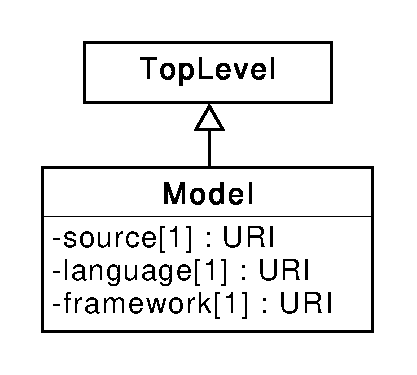
\includegraphics[scale=0.6]{uml/model}
\caption[]{Diagram of the \sbol{Model} class and its associated properties.}
\label{uml:model}
\end{center}
\end{figure}

The purpose of the \sbol{Model} class is to serve as a placeholder for an external model and provide additional meta-data to enable better reasoning about the contents of this model.
In this way, there is minimal duplication of standardization efforts and users of SBOL can specify the quantitative function of a \sbol{ModuleDefinition} in the language of their choice. 

The meta-data provided by the \sbol{Model} class include the following properties: the \sbol{source} or location of the actual content of the model, the \sbol{language} in which the model is implemented, and the model's mathematical \sbol{framework}. 

\subsubsection*{ The \sbolheading{source} property}\label{sec:source}
The \sbol{source} property is REQUIRED and MUST contain a \external{URI} reference to a qualitative or quantitative model.

\subsubsection*{ The \sbolheading{language} property}\label{sec:language}
The \sbol{language} property is REQUIRED and MUST contain a \external{URI} that specifies the language in which the model is implemented. It is RECOMMENDED that this \external{URI} refer to a term from the EMBRACE Data and Methods (EDAM) ontology. \ref{tbl:model_types} provides a list of RECOMMENDED terms from this ontology and their \external{URI}s. If the \sbol{language} property of a \sbol{Model} is well-described by one these terms, then it MUST  use the \external{URI} for this term as its value.

\begin{table}[ht]
  \begin{edtable}{tabular}{ll}
    \toprule
    \textbf{Model Language} & \textbf{URI} \\
    \midrule
    SBML  & \url{http://identifiers.org/edam/format_2585}\\
    CellML		 & \url{http://identifiers.org/edam/format_3240}\\
    BioPAX    & \url{http://identifiers.org/edam/format_3156}\\
    \bottomrule
  \end{edtable}
  \caption{RECOMMENDED terms from the EDAM ontology to specify the \sbol{language} property of a \sbol{Model}.}
  \label{tbl:model_types}
\end{table}


\subsubsection*{ The \sbolheading{framework} property}\label{sec:framework}
This REQUIRED property is a URI that specifies the modeling framework that a model is implemented within. 
Values for this URI are RECOMMENDED to be chosen from the SBO's modeling framework terms where possible. A few suggested model frameworks and corresponding URI values are shown in \ref{tbl:model_frameworks}.

\begin{table}[ht]
  \begin{edtable}{tabular}{ll}
    \toprule
    \textbf{Framework} & \textbf{URI} \\
    \midrule
    Continuous  & \url{http://identifiers.org/biomodels.sbo/SBO:0000062}\\
    Discrete & \url{http://identifiers.org/biomodels.sbo/SBO:0000063}\\
    \bottomrule
  \end{edtable}
  \caption{Example modelling frameworks and corresponding SBO terms.}
  \label{tbl:model_frameworks}
\end{table}

\subsubsection*{Serialization}

The serialization of a \sbol{Model} MUST have the following form:

\lstsetsbol
\begin{lstlisting}
<sbol:Model rdf:about="http://www.sbolstandard.org/examples/toogleswicth">
  ... [\emph{properties inherited from identified}] ...
  [\emph{one}] <sbol:source rdf:resource="..."/> [\emph{element}]
  [\emph{one}] <sbol:language rdf:resource="..."/> [\emph{element}]
  [\emph{one}] <sbol:framework rdf:resource="..."/> [\emph{element}]
</sbol:Model>
\end{lstlisting}

The example below shows the serialization of a \sbol{Model} object that refers to a quantitative model of a genetic toggle switch. The model is implemented in the SBML \sbol{language} and adheres to a continuous modeling \sbol{framework}. Lastly, the model can be retrieved from a model repository via its \sbol{source} \external{URI}, which is a \external{URL}.
\lstsetsbol
\begin{lstlisting}
<?xml version="1.0" ?>
<rdf:RDF xmlns:rdf="http://www.w3.org/1999/02/22-rdf-syntax-ns#" xmlns:dcterms="http://purl.org/dc/terms/" xmlns:prov="http://www.w3.org/ns/prov#" xmlns:sbol="http://sbols.org/v2#">
  <sbol:Model rdf:about="http://www.sbolstandard.org/examples/pIKE_Toggle_1">
    <sbol:persistentIdentity rdf:resource="http://www.sbolstandard.org/examples/pIKE_Toggle_1"/>
    <sbol:displayId>pIKE_Toggle_1</sbol:displayId>
    <dcterms:title>pIKE_Toggle_1 toggle switch</dcterms:title>
    <sbol:source rdf:resource="http://virtualparts.org/part/pIKE_Toggle_1"/>
    <sbol:language rdf:resource="http://identifiers.org/edam/format_2585"/>
    <sbol:framework rdf:resource="http://identifiers.org/biomodels.sbo/SBO:0000062"/>
  </sbol:Model>
</rdf:RDF>
\end{lstlisting}
\label{ser:Model}

\subsection{ModuleDefinition}
\label{sec:ModuleDefinition}

\begin{figure}[ht]
\begin{center}
\includegraphics[scale=0.6]{uml/module_definition}
\caption[]{Diagram of the \sbol{ModuleDefinition} class and its associated properties.}
\label{uml:module_definition}
\end{center}
\end{figure}

The \sbol{ModuleDefinition} class is the hub where the structural and functional aspects of genetic designs are brought together to form a complete picture of the design. 
A \sbol{ModuleDefinition} object is composed from zero or more \sbol{FunctionalComponent}, \sbol{Module}, and \sbol{Interaction} objects, and links to zero or more \sbol{Model} objects. 

As an engineering object, a \sbol{ModuleDefinition} will often have certain of its \sbol{FunctionalComponent} objects that are intended to carry signals in or out of it.  
This functionality of designated ``inputs'' and ``outputs'' is expressed by \sbol{direction} properties on its \sbol{FunctionalComponent} elements.

\subsubsection*{The \sbolheading{roles} property}\label{sec:roles:MD}
The \sbolmult{roles:MD}{roles} property is an OPTIONAL set of \sbol{URI}s that clarifies the intended function of a \sbol{ModuleDefinition} in a biological context.  

These terms might identify ``logical'' roles, such as ``inverter'' or ``AND gate'', or they might identify descriptive biological roles, such as ``metabolic pathway'' and ``signaling cascade,'' or might identify roles from some other manner of describing intended function.
Interpretation of the meaning of such roles is currently implementation-dependent.

\subsubsection*{The \sbolheading{modules} property}\label{sec:modules}

The \sbol{modules} property is OPTIONAL and MAY specify a set of \sbol{Module} objects contained by the \sbol{ModuleDefinition}.
Note that the set of relations between \sbol{Module} and \sbol{ModuleDefinition} objects is strictly acyclic.

While the \sbol{ModuleDefinition} class is analogous to a blueprint or specification sheet for a system of interaction biological elements, the \sbol{Module} class represents the specific occurrence of a particular sub-system within that design. 
Hence, this class allows a biological design to include multiple instances of a subsystem (defined by reference to the same \sbol{ModuleDefinition}).
For example, the \sbol{ModuleDefinition} for a network of two-input repressor systems, where the particular repressors have not yet been chosen, contain multiple \sbol{Module} objects that refer to the same \sbol{URI} for the \sbol{ModuleDefinition} of an abstract two-input repressor device.

\subsubsection*{The \sbolheading{functionalComponents} property}
\label{sec:functionalComponents}

The \sbol{functionalComponents} property is OPTIONAL and MAY specify a set of \sbol{FunctionalComponent} objects contained by the \sbol{ModuleDefinition}.

Just as a \sbol{Module} represents an instance of a subsystem in the  \sbol{ModuleDefinition} "blueprint", a \sbol{FunctionalComponent} represents an instance of an individual element whose \sbol{ComponentDefinition} may be used multiple times in a \sbol{ModuleDefinition}.  For example, a \sbol{ModuleDefinition} might contain several copies of a particular promoter.

\subsubsection*{The \sbolheading{interactions} property}\label{sec:interactions}

The \sbol{interactions} property is OPTIONAL and MAY specify a set of \sbol{Interaction} objects within a \sbol{ModuleDefinition}.

The \sbol{Interaction} class provides an abstract, machine-friendly representation of the functional interactions of entities within a \sbol{ModuleDefinition} (whereas a \sbol{Model} of a system may not be readily susceptible to machine reasoning, depending on how it is implemented).  
Each \sbol{Interaction} includes \sbol{Participation} entities that indicate the roles of the \sbol{FunctionalComponent} objects involved in the \sbol{Interaction}

\subsubsection*{The \sbolheading{models} property}\label{sec:models}
The \sbol{models} property is OPTIONAL and MAY specify a set of \sbol{URI}s identifying \sbol{Model} objects.

SBOL's \sbol{Model} objects are placeholders used to link specifications of biological parts and their interactions to computational models of arbitrary format.
A \sbol{ModuleDefinition} object can link to more than one \sbol{Model} since each might encode the same system in a different way or at a different level of detail.

\subsubsection*{Serialization}

The serialization of \sbol{ModuleDefinition} has the following form:
\lstsetsbol
\begin{lstlisting}
<sbol:ModuleDefinition rdf:about="...">
  ... [\emph{properties inherited from identified}] ...
  [\emph{zero or more}]  <sbol:role rdf:resource="..."/> [\emph{elements}]
  [\emph{zero or more}]  <sbol:model rdf:resource="..."/> [\emph{elements}]
  [\emph{zero or more}] <sbol:functionalComponent>
                 <sbol:FunctionalComponent rdf:about="...">...</sbol:FunctionalComponent >
               </sbol:functionalComponent> [\emph{elements}]
  [\emph{zero or more}] <sbol:module>
                 <sbol:Module rdf:about="...">...</sbol:Module>
               </sbol:module> [\emph{elements}]
  [\emph{zero or more}] <sbol:interaction>
                 <sbol:Interaction rdf:about="...">...</sbol:Interaction>
               </sbol:interaction> [\emph{elements}]
</sbol:ModuleDefinition>
\end{lstlisting}

The example below shows a simple \sbol{ModuleDefinition} containing two components, a \sbol{FunctionalComponent} for a DNA sequence encoding constitutive expression of GFP and another for the GFP protein expressed from this sequence, plus an interaction describing that relation.

\lstsetsbol
\begin{lstlisting}
<sbol:ModuleDefinition rdf:about="http://sbolstandard.org/example/md/GFP_expression">
  <sbol:functionalComponent>
    <sbol:FunctionalComponent rdf:about="http://sbolstandard.org/example/md/GFP_expression/GFP_protein">
      <sbol:definition rdf:resource="http://sbolstandard.org/example/GFP"/>
      <sbol:access rdf:resource="http://sbols.org/v2#public"/>
      <sbol:direction rdf:resource="http://sbols.org/v2#output"/>
    </sbol:FunctionalComponent>
  </sbol:functionalComponent>
  <sbol:functionalComponent>
    <sbol:FunctionalComponent rdf:about="http://sbolstandard.org/example/md/GFP_expression/Constitutive_GFP">
      <sbol:definition rdf:resource="http://sbolstandard.org/example/GFP_generator"/>
      <sbol:access rdf:resource="http://sbols.org/v2#public"/>
      <sbol:direction rdf:resource="http://sbols.org/v2#none"/>
    </sbol:FunctionalComponent>
  </sbol:functionalComponent>
  <sbol:interaction>
    <sbol:Interaction rdf:about="http://sbolstandard.org/example/md/GFP_expression/express_GFP">
      ...
    </sbol:Interaction>
  </sbol:interaction>
</sbol:ModuleDefinition>
\end{lstlisting}

\subsubsection{FunctionalComponent}
\label{sec:FunctionalComponent}
A \sbol{FunctionalComponent} is an instance of a \sbol{ComponentDefinition} being used as part of a \sbol{ModuleDefinition} object.
Each \sbol{FunctionalComponent} object is owned by a \sbol{ModuleDefinition} object and represents an explicit usage of a \sbol{ComponentDefinition} object for the purpose of fulfilling some function. 

\sbol{FunctionalComponent} derives from \sbol{ComponentInstance}, and therefore has the \sbolmult{definition:CI}{definition}, \sbol{access}, and \sbolmult{mapsTos:CI}{mapsTos} properties. 
Additionally, it has a \sbol{direction} property that specifies whether it serves as an input, output, both, or neither with regards to the \sbol{ModuleDefinition} that contains it.

\paragraph{The \sbolheading{direction} property}\label{sec:direction}
Each \sbol{FunctionalComponent} MUST specify via the \sbol{direction} property whether it serves as an  input, output, both, or neither for its parent \sbol{ModuleDefinition} object. 
The value for this property MUST be one of the values given in \ref{tbl:functionalcomponent_directions}.


\begin{table}[ht]
  \begin{edtable}{tabular}{ll}
    \toprule
    \textbf{Direction URI} & \textbf{Description} \\
    \midrule
    \url{http://sbols.org/v2#inout}  & To indicate a \sbol{FunctionalComponent} can be used as both input or output\\
    \url{http://sbols.org/v2#in}  & To indicate a \sbol{FunctionalComponent} can be used as input\\
    \url{http://sbols.org/v2#out}  & To indicate a \sbol{FunctionalComponent} can be used as output\\
    \url{http://sbols.org/v2#none}  & To indicate a \sbol{FunctionalComponent} is neither input nor output\\
    \bottomrule
  \end{edtable}
  \caption{\sbol{URI}s for the \sbol{direction} property.}
  \label{tbl:functionalcomponent_directions}
\end{table}

The \sbol{direction} property is a means to encode a common way in which designers think about the ``purpose'' of a connection in a system.  In this case, the connection is the \sbol{FunctionalComponent}, and the system is the \sbol{ModuleDefinition}.
For example, consider a system that is designed to indicate concentration of the cell-cell signalling molecule 3OC$_6$HSL by the concentration of the product of a particular CDS.
In this system, the concentration of 3OC$_6$HSL is the signal being interpreted by the system, so the \sbol{FunctionalComponent} for 3OC$_6$HSL would have a \sbol{direction} of ``input.''  
Complementarily, the concentration of the designated product is the signal intended for consumption by other biologicals systems, and so the \sbol{FunctionalComponent} for that product would have a \sbol{direction} of ``output.''
The CDS encoding the product, however, is not intended to interact directly, and so its \sbol{FunctionalComponent} would have a \sbol{direction} of ``neither.''
Finally, in some cases a \sbol{FunctionalComponent} may serve as both an input and output, and be marked as having a \sbol{direction} of ``both.''

\paragraph{Serialization}

The serialization of \sbol{FunctionalComponent}s has the following form.
\lstsetsbol
\begin{lstlisting}
<sbol:FunctionalComponent rdf:about="...">
  ... [\emph{properties inherited from identified}] ...
  [\emph{one}]          <sbol:definition rdf:resource="..."/> [\emph{element}]
  [\emph{one}]          <sbol:access rdf:resource="..."/> [\emph{element}]
  [\emph{one}]          <sbol:direction rdf:resource="..."/> [\emph{element}]
  [\emph{zero or more}] <sbol:mapsTo rdf:resource="..."/> [\emph{elements}]
</sbol:FunctionalComponent>
\end{lstlisting}

In the example below, the functional component is defined as public input or output. The component refers to the \texttt{Part:BBa\_R0010} promoter from the Parts Registry.
\lstsetsbol
\begin{lstlisting}
<sbol:FunctionalComponent rdf:about="http://sbolstandard.org/example/laci_inverter/promoter">
  <sbol:definition rdf:resource="http://www.partsregistry.org/BBa_R0010"/>
  <sbol:access rdf:resource="http://sbols.org/v2#public"/>
  <sbol:direction rdf:resource="http://sbols.org/v2#inout"/>
</sbol:FunctionalComponent>
\end{lstlisting}

\subsubsection{Module}
\label{sec:Module}

\begin{figure}[ht]
\begin{center}
\includegraphics[scale=0.6]{uml/module}
\caption[]{Diagram of the \sbol{Module} class and its associated properties.}
\label{uml:module}
\end{center}
\end{figure}

The \sbol{Module} class represents the usage or occurrence of a \sbol{ModuleDefinition} within a larger design (that is, another \sbol{ModuleDefinition}).  

\paragraph{The \sbolheading{definition} property}
\label{sec:definition:M}

The \sbolmult{definition:M}{definition} property is a REQUIRED \sbol{URI} that refers to the \sbol{ModuleDefinition} for the \sbol{Module}.

The \sbolmult{definition:M}{definition} property MUST NOT refer to the same \sbol{ModuleDefinition} as that which contains the \sbol{Module}. 
Furthermore, \sbol{Module} objects MUST NOT form a cyclical chain of references via their \sbolmult{definition:M}{definition} properties and the \sbol{ModuleDefinition} objects that contain them. For example, consider the \sbol{Module} objects $A$ and $B$ and the \sbol{ModuleDefinition} objects $X$ and $Y$. The reference chain ``$X$ contains $A$, $A$ is defined by $Y$, $Y$ contains $B$, and $B$ is defined by $X$'' is cyclical. 

\paragraph{The \sbolheading{mapsTo} property}
\label{sec:mapsTos:M}

The \sbolmult{mapsTos:M}{mapsTos} property is an OPTIONAL set of \sbol{MapsTo} objects that refer to and link \sbol{Module} objects together within a larger design.

\ref{sec:MapsTo} contains a detailed description of the \sbol{MapsTo} class.

\paragraph{Serialization}
The serialization of \sbol{Module}s has the following form.
\lstsetsbol
\begin{lstlisting}
<sbol:Module rdf:about="...">
  ... [\emph{properties inherited from identified}] ...
  [\emph{one}]          <sbol:definition rdf:resource="..."/> [\emph{element}]
  [\emph{zero or more}] <sbol:mapsTo>
                 <sbol:MapsTo rdf:about="...">...</sbol:MapsTo>
               </sbol:mapsTo> [\emph{element}]
</sbol:Module>
\end{lstlisting}

The example below specifies a TetR inverter that is being used as
a part of a toggle switch:

\lstsetsbol
\begin{lstlisting}
<sbol:Module rdf:about="http://sbolstandard.org/example/toggle_switch/tetr_inverter">
  <sbol:definition rdf:resource="http://sbolstandard.org/example/tetr_inverter"/>
  ...
</sbol:Module>
\end{lstlisting}

\subsubsection{Interaction}
\label{sec:Interaction}

\begin{figure}[ht]
\begin{center}
\includegraphics[scale=0.6]{uml/interaction}
\caption[]{Diagram of the \sbol{Interaction} class and its associated properties.}
\label{uml:interaction}
\end{center}
\end{figure}

The \sbol{Interaction} class provides a description of the functional interactions of entities within a \sbol{ModuleDefinition}.
For example, it can be used to represent regulatory interactions, such as activation or repression, processes from the central dogma of biology, such as transcription and translation, or molecular interactions like  non-covalent binding between a small molecule and transcription factor or phosphorylation of a transcription factor by an enzyme.
Such an \sbol{Interaction} is represented in SBOL by referring to an ontology defining the type of interaction and declaring how various entities participate in the interaction.

\paragraph{The \sbolheading{types} property}\label{sec:types:I}

The \sbolmult{types:I}{types} property is a REQUIRED set of one or more \sbol{URI}s that identify an appropriate ontology term describing the behavior represented by this \sbol{Interaction}. 
If an \sbol{Interaction} object has multiple
\sbolmult{types:I}{types} \sbol{URI}s, then they must identify synonymous terms.

Values for this URI are RECOMMENDED to be chosen from the occurring entity branch of the Systems Biology Ontology (SBO), where possible.
(See \url{http://www.ebi.ac.uk/sbo/main/})

\paragraph{The \sbolheading{participations} property}\label{sec:participations}

The \sbol{participations} property is an OPTIONAL set of \sbol{Participation} objects, each of which identifies the \sbolmult{roles:P}{roles} that the referenced \sbol{FunctionalComponent} plays in the interaction.

Note that even though an \sbol{Interaction} generally involves at least one \sbol{Participation}, the case of zero participations is allowed because it is plausible that a design may wish to specify that an \sbol{Interaction} will exist, even if its \sbol{participant}s are not yet determined.

\paragraph{Serialization}

The serialization of \sbol{Interaction} objects has the following form.
\lstsetsbol
\begin{lstlisting}
<sbol:Interaction rdf:about="...">
  ... [\emph{properties inherited from identified}] ...
  [\emph{one or more}]  <sbol:type rdf:resource="..."/> [\emph{elements}]
  [\emph{zero or more}] <sbol:participation>
                 <sbol:Participation rdf:about="...">...</sbol:Participation>
               </sbol:participation> [\emph{elements}]
</sbol:Interaction>
\end{lstlisting}

The example below shows an \sbol{Interaction} representing an inhibition relationship (SBO:0000169) between a repressor (SBO:0000020, full \sbol{Participation} details shown) and a promoter:

\lstsetsbol
\begin{lstlisting}
<sbol:Interaction rdf:about="http://sbolstandard.org/example/laci_inverter/LacI_pLacI">
  <sbol:type rdf:resource="http://identifiers.org/biomodels.sbo/SBO:0000169"/>
  <sbol:participation>
    <sbol:Participation rdf:about="http://sbolstandard.org/example/laci_inverter/LacI_pLacI/P03023">
      <sbol:role rdf:resource="http://identifiers.org/biomodels.sbo/SBO:0000020"/>
      <sbol:participant rdf:resource="http://sbolstandard.org/example/laci_inverter/TF"/>
    </sbol:Participation>
  </sbol:participation>
  <sbol:participation>
    <sbol:Participation rdf:about="...">
      ... 
    </sbol:Participation>
  </sbol:participation>
</sbol:Interaction>
\end{lstlisting}


\begin{figure}[ht]
\begin{center}
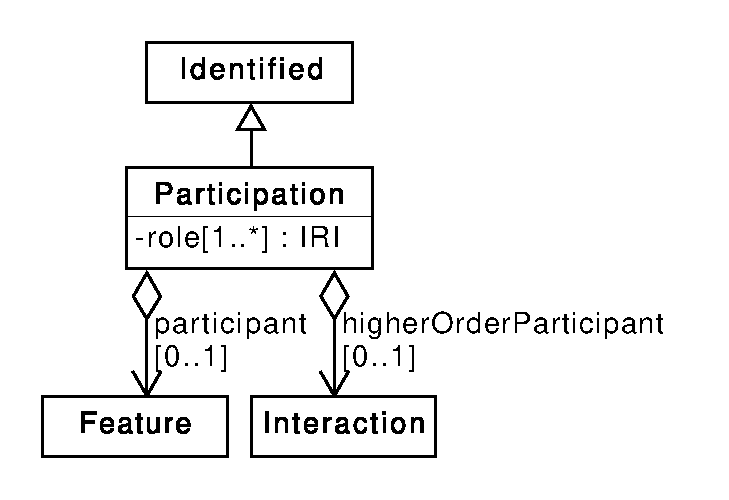
\includegraphics[scale=0.6]{uml/participation}
\caption[]{Diagram of the \sbol{Participation} class and its associated properties.}
\label{uml:participation}
\end{center}
\end{figure}

\subsubsection{Participation}
\label{sec:Participation}

Each \sbol{Participation} object describes the role or roles that a
particular \sbol{FunctionalComponent} plays in its parent
\sbol{Interaction}.

\paragraph{The \sbolheading{roles} property}\label{sec:roles:P}

The \sbolmult{roles:P}{roles} property is an OPTIONAL set of \sbol{URI}s that identify an appropriate ontology term describing this elements relationship to its parent \sbol{Interaction}. 
If a \sbol{Participation} object has multiple
\sbolmult{roles:P}{roles} \sbol{URI}s, then they must identify synonymous terms.

Values for this URI are RECOMMENDED to be chosen from the participant role branch of the Systems Biology Ontology (SBO) where possible.
(See \url{http://www.ebi.ac.uk/sbo/main/})

\paragraph{The \sbolheading{participant} property}\label{sec:participant}

The \sbol{participant} property MUST specify precisely one \sbol{FunctionalComponent} object that plays the designated \sbolmult{roles:P}{roles} in its parent \sbol{Interaction} object.


\paragraph{Serialization}

The serialization of \sbol{Participation} objects has the following form.
\lstsetsbol
\begin{lstlisting}
<sbol:Participation rdf:about="...">
  ... [\emph{properties inherited from identified}] ...
  [\emph{zero or more}] <sbol:role rdf:resource="..."/> [\emph{elements}]
  [\emph{one}]          <sbol:participant rdf:resource="..."/> [\emph{element}]
</sbol:Participation>
\end{lstlisting}

In the example below, the role of participating \sbol{FunctionalComponent} is defined to be \external{inhibitor}, using the \external{SBO:0000020} term. This component is specified using the participant property of the \sbol{Participation} entity.
\lstsetsbol
\begin{lstlisting}
<sbol:Participation rdf:about="http://sbolstandard.org/example/laci_inverter/LacI_pLacI/P03023">
  <sbol:role rdf:resource="http://identifiers.org/biomodels.sbo/SBO:0000020"/>
  <sbol:participant rdf:resource="http://sbolstandard.org/example/laci_inverter/TF"/>
</sbol:Participation>
\end{lstlisting}

\subsection {Collection}
\label{sec:Collection}
The \sbol{Collection} class is a class that groups together a set of \sbol{TopLevel} objects that have something in common. 
Some examples of \sbol{Collection} objects:
\begin{itemize}
\item Results of a query to find all \sbol{ComponentDefinition} objects that function as promoters in a repository.
\item A set of \sbol{ModuleDefinition} objects representing a library of NAND gates.
\item A \sbol{ModuleDefinition} for a complex design, and all of the \sbol{ModuleDefinition}, \sbol{ComponentDefinition}, \sbol{Sequence}, and \sbol{Model} objects used to provide its full specification.
\end{itemize}

\begin{figure}[ht]
\begin{center}
\includegraphics[scale=0.6]{uml/collection}
\caption[]{Diagram of the \sbol{Collection} class and its associated properties.}
\label{uml:collection}
\end{center}
\end{figure}

\subsubsection*{The \sbolheading{members} property}\label{sec:members}
The \sbol{members} property has a data type of URI and has the URI for a \sbol{TopLevel} entity.  A \sbol{Collection} may have any number of members, including none.

\subsubsection*{Serialization}

The serialization of \sbol{Collection} objects has the following form:

\lstsetsbol
\begin{lstlisting}
<sbol:Collection rdf:about="...">
  ... [\emph{properties inherited from identified}] ...
  [\emph{zero or more}] <sbol:member rdf:resource="..."/> [\emph{element}]
</sbol:Collection>
\end{lstlisting}

The example below shows the serialization of a \sbol{Collection} object grouping together a library of constitutive promoters.
\lstsetsbol
\begin{lstlisting}
<?xml version="1.0" ?>
<rdf:RDF xmlns:rdf="http://www.w3.org/1999/02/22-rdf-syntax-ns#" xmlns:dcterms="http://purl.org/dc/terms/" xmlns:prov="http://www.w3.org/ns/prov#" xmlns:sbol="http://sbols.org/v2#">
  <sbol:Collection rdf:about="http://parts.igem.org/Promoters/Catalog/Anderson">
    <sbol:persistentIdentity rdf:resource="http://parts.igem.org/Promoters/Catalog/Anderson"/>
    <sbol:displayId>Anderson</sbol:displayId>
    <dcterms:title>Anderson promoters</dcterms:title>
    <dcterms:description>The Anderson promoter collection</dcterms:description>
    <sbol:member rdf:resource="http://partsregistry.org/Part:BBa_J23119"/>
    ...
    <sbol:member rdf:resource="http://partsregistry.org/Part:BBa_J23118"/>
  </sbol:Collection>
</rdf:RDF>
\end{lstlisting}
\label{ser:Collection}

\subsection{SBOL Extension Mechanism}
\label{sec:Annotations}
\label{sec:annotations}

SBOL does not attempt to represent all information about a biological system, since many things do not yet have a clear ``right way'' to be represented, such as design intent, biological context, or performance data.  Instead, SBOL allows the embedding of application specific data that are not captured by the SBOL standard.  Such data are optional, but can be computationally generated and exchanged via SBOL documents without getting damaged or lost. This SBOL extension mechanism is designed to allow easy incorporation within the SBOL standard once there is community agreement on data content to be exchanged.

To do this, SBOL provides an ``annotation'' mechanism for attaching arbitrary information to SBOL objects, which allows SBOL models to be connected with any other models in an extensible manner.
In particular, several methods are supported for connecting the SBOL data model with other, possibly application-specific data:
\begin{enumerate}
\item Information that is ``part'' of an SBOL object (i.e., a ``filled diamond'' relationship) is annotated simply by adding non-conflicting properties and custom entries to an SBOL object.  An example might be source information about the registry from which a \sbol{ComponentDefinition} was imported.
\item Information that is an independent object is annotated by wrapping it inside of a \sbol{GenericTopLevel} object.  An example might be a data sheet describing the performance of a \sbol{ModuleDefinition} in some particular context.
\item Conversely, rather than embedding external objects in SBOL, SBOL objects can also be linked to external data.  The only requirement is that some URI resolution mechanism must be available that allows the links from SBOL objects to be followed when needed.
\item Finally, just as external objects can be embedded in SBOL, external documents can embed or refer to SBOL objects.  This last case needs no explicit support from this specification (it depends only on the external non-SBOL system managing its own relations to SBOL), and is included here for completeness.
\end{enumerate}

\subsubsection{Annotating SBOL objects}
% whole set of labels for the properties defined herein
\label{sec:qName}
\label{sec:QName}
\label{sec:value}
\label{sec:Annotation}
\label{sec:AnnotationValue}
\label{sec:NestedAnnotations}
\label{sec:nestedQName}
\label{sec:nestedURI}

Each \sbol{Identified} object may have a number of annotations in the form of name/value property pairs. The \sbol{qName} property is specified by a qualified name (\sbol{QName}), which is composed of a namespace, a prefix, and a local name. The \sbol{qName} property must be stored in the data model to allow for proper serialization as described below.
The \sbol{value} property can be a literal type (i.e., \sbol{String}, \sbol{Integer}, \sbol{Double}, \sbol{Boolean}), \sbol{URI}, or a \sbol{NestedAnnotations} object. The \sbol{NestedAnnotations} object is composed of a \sbol{nestedQName}, \sbol{nestedURI}, and an optional list of nested \sbol{annotations}.


\begin{figure}[!ht]
\begin{center}
\includegraphics[scale=0.6]{uml/identified_annotations}
\caption[]{Diagram of the \sbol{Annotation} class and its association with \sbol{Identified} and \sbol{AnnotationValue} objects, which is used for annotating SBOL entities with application specific data.}
\label{uml:identified_annotations}
\end{center}
\end{figure}

\subsubsection*{Serialization}


The serialization of \sbol{Annotation} objects has the following form:

\lstsetsbol
\begin{lstlisting}
<?xml version="1.0" ?>
<rdf:RDF xmlns:rdf="http://www.w3.org/1999/02/22-rdf-syntax-ns#" 
  xmlns:sbol="http://sbols.org/v2#"
  xmlns:prefix1="NAMESPACE_1" 
  xmlns:prefix2="NAMESPACE_2" 
  xmlns:nestedObjectPrefix="A_NESTED_OBJECT_NAMESPACE" 
  ...
 >
<sbol:A_TOPLEVELOBJECT rdf:about="...">
                ...
  [\emph{zero or more}] <prefix1:LOCAL_NAME_1>A_LITERAL</prefix1:LOCAL_NAME_1> [\emph{elements}]
  [\emph{zero or more}] <prefix1:LOCAL_NAME_2 rdf:resource=URI/> [\emph{elements}]
  [\emph{zero or more}] <prefix2:LOCAL_NAME_3>
                  <nestedObjectPrefix:NESTED_LOCAL_NAME rdf:about="...">
                    ...
                  </nestedObjectPrefix:NESTED_LOCAL_NAME>
                </prefix2:LOCAL_NAME_3> [\emph{elements}]
</sbol:TOPLEVELOBJECT>
\end{lstlisting}
The \sbol{qName} property specifies the namespace, prefix, and localPart values.  The use of such qualified names is described in detail by the w3c here:\\
\url{http://www.w3.org/TR/1999/REC-xml-names-19990114/#ns-using}\\
Essentially, the "xmlns" statement defines the prefix string to use as an alias for the namespace.  The prefix can be any arbitrary string, and its use is optional, since it simply replaces the full namespace making the serialization more readable.

The first annotation shown above is for a \sbol{literal} annotation.  The second form is for a \sbol{URI} annotation.  Finally, the third form is for an \sbol{NestedAnnotations} object annotation.  In this last case, the \sbol{nestedQName} property specifies the nestedNamespace, nestedPrefix, and nestedLocalPart while the \sbol{nestedURI} property species the URI for the nested annotation.

The ComponentDefinition example for a promoter serialized below shows how annotations can be added to SBOL objects. Annotations are added using the relevant information from the Parts Registry. Annotation property names are qualified with the \external{http://www.partsregistry.org/} namespace, which is prefixed using \external{pr}. The first annotation is named as \external{pr:group}, indicating the iGEM group designing the promoter, and has a \sbol{String} value. 
The second \external{pr:experience} annotation has a \sbol{URI} value and is serialised as an RDF resource; in this case, the identifier also happens to be able to be resolved to the information Web page on the Parts Registry for the promoter. 
The  \external{pr:information} property represents a complex annotation which is a type of \external{pr:Information} and includes information about the regulatory details of the promoter using Parts Registry categories.   

\begin{figure} [ht]
\lstsetsbol
\begin{lstlisting}
<?xml version="1.0" ?>
<rdf:RDF xmlns:pr="http://partsregistry.org" xmlns:rdf="http://www.w3.org/1999/02/22-rdf-syntax-ns#" xmlns:dcterms="http://purl.org/dc/terms/" xmlns:prov="http://www.w3.org/ns/prov#" xmlns:sbol="http://sbols.org/v2#">
  <sbol:ComponentDefinition rdf:about="http://partsregistry.org/cd/BBa_J23119">
    <sbol:persistentIdentity rdf:resource="http://partsregistry.org/cd/BBa_J23119"/>
    <sbol:displayId>BBa_J23119</sbol:displayId>
    <pr:group>iGEM2006_Berkeley</pr:group>
    <pr:experience rdf:resource="http://parts.igem.org/cgi/partsdb/part_info.cgi?part_name=BBa_J23119"/>
    <pr:information>
      <pr:Information rdf:about="http://parts.igem.org/cgi/partsdb/part_info.cgi?part_name=BBa_J23119">
        <pr:sigmafactor>//rnap/prokaryote/ecoli/sigma70</pr:sigmafactor>
        <pr:regulation>//regulation/constitutive</pr:regulation>
      </pr:Information>
    </pr:information>
    <dcterms:title>J23119</dcterms:title>
    <dcterms:description>Constitutive promoter</dcterms:description>
    <sbol:type rdf:resource="http://www.biopax.org/release/biopax-level3.owl#DnaRegion"/>
    <sbol:role rdf:resource="http://identifiers.org/so/SO:0000167"/>
  </sbol:ComponentDefinition>
</rdf:RDF>
\end{lstlisting}
\label{ser:Annotation}
\end{figure}

\subsubsection{GenericTopLevel}  
\label{sec:GenericTopLevel}
\label{sec:rdfType}

SBOL documents can also be annotated at the top level. 
SBOL's \sbol{GenericTopLevel} is a top-level entity whose only purpose is to include a set of annotations as described above. 
Entities that have independent existence (i.e., would be another ``top level'' class) and are not recognized by the SBOL standard are loaded into these top level entities. 
These \sbol{GenericTopLevel} entities can thus be safely used by tools to exchange non-SBOL data embedded separately within SBOL.
As with any other top level entities, \sbol{GenericTopLevel} entities may include SBOL properties such as \sbol{displayId}, \sbol{name}, \sbol{description}, etc. The type of data found in the generic entity is indicated using the \sbol{rdfType} property which is of type \sbol{QName}.  Again, the \sbol{rdfType} property is used to set the prefix and localPart fields during serialization.

\begin{figure}[ht]
\begin{center}
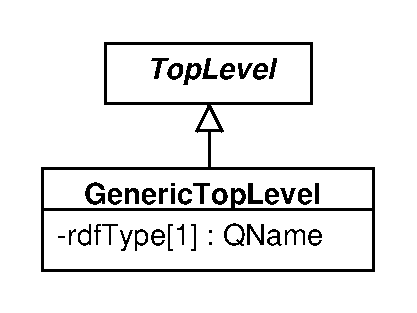
\includegraphics[scale=0.6]{uml/generictoplevel}
\caption[]{Diagram of the \sbol{GenericTopLevel} class and its associated properties, which is used for embedding externally defined entities into SBOL documents.}
\label{uml:generictoplevel}
\end{center}
\end{figure}

\subsubsection*{Serialization}

The serialization of \sbol{GenericTopLevel} objects has the following form where the prefix, namespace, and localPart are defined by the \sbol{rdfType} property:

%<?xml version="1.0" ?>
%<rdf:RDF ... xmlns:prefix=namespace ...>
%<prefix:localPart rdf:about="...">
%              ...
%</prefix:localPart>

\lstsetsbol
\begin{lstlisting}
<?xml version="1.0" ?>
<rdf:RDF xmlns:rdf="http://www.w3.org/1999/02/22-rdf-syntax-ns#" 
  xmlns:sbol="http://sbols.org/v2#"
  xmlns:applicationPrefix="APPLICATION_NAMESPACE" 
  ...
 >
<applicationPrefix:APPLICATION_OBJECT_NAME rdf:about="...">
  ... [\emph{properties inherited from identified}] ...
  ... [\emph{any non-conflicting application-specific properties}] ...
</applicationPrefix:APPLICATION_OBJECT_NAME>
\end{lstlisting}

The example below shows how a datasheet object can be added to an SBOL document using the \sbol{GenericTopLevel} class. 
The J23119 promoter example is annotated with the URI of a top Level Datasheet object, here defining the annotation properties using the custom \external{\path{http://www.myapp.org/}} namespace and the \external{myapp} prefix. 
The datasheet object, with the data type of \external{myapp:Datasheet}, is accessed using the \sbol{URI} specified by the \external{myapp:characterizationData} property of the promoter \sbol{ComponentDefinition}. 
The datasheet object is further annotated with the transcription rate and URI for the actual characterization data using the \external{myapp:transcriptionRate} and \external{myapp:characterizationData} properties, respectively.
Finally, this data sheet is linked from the component it describes using an annotation with a \external{myapp:datasheet} property whose value is the datasheet's URI.

\begin{figure}[ht]
\lstsetsbol
\begin{lstlisting}
<?xml version="1.0" ?>
<rdf:RDF xmlns:myapp="http://www.myapp.org/" xmlns:rdf="http://www.w3.org/1999/02/22-rdf-syntax-ns#" xmlns:dcterms="http://purl.org/dc/terms/" xmlns:prov="http://www.w3.org/ns/prov#" xmlns:sbol="http://sbols.org/v2#">
  <sbol:ComponentDefinition rdf:about="http://www.partsregistry.org/cd/BBa_J23119">
    <sbol:persistentIdentity rdf:resource="http://www.partsregistry.org/cd/BBa_J23119"/>
    <sbol:displayId>BBa_J23119</sbol:displayId>
    <prov:wasDerivedFrom rdf:resource="http://www.partsregistry.org/Part:BBa_J23119"/>
    <myapp:datasheet rdf:resource="http://www.partsregistry.org/gen/datasheet1"/>
    <dcterms:title>J23119</dcterms:title>
    <dcterms:description>Constitutive promoter</dcterms:description>
    <sbol:type rdf:resource="http://www.biopax.org/release/biopax-level3.owl#DnaRegion"/>
    <sbol:role rdf:resource="http://identifiers.org/so/SO:0000167"/>
  </sbol:ComponentDefinition>
  <myapp:Datasheet rdf:about="http://www.partsregistry.org/gen/datasheet1">
    <sbol:persistentIdentity rdf:resource="http://www.partsregistry.org/gen/datasheet1"/>
    <sbol:displayId>datasheet1</sbol:displayId>
    <myapp:characterizationData rdf:resource="http://www.myapp.org/measurement/1"/>
    <myapp:transcriptionRate>1</myapp:transcriptionRate>
    <dcterms:title>Datasheet 1</dcterms:title>
  </myapp:Datasheet>
</rdf:RDF>
\end{lstlisting}
\label{ser:GenericTopLevel}
\end{figure}

\section{Mapping Between SBOL 1.1 and SBOL 2.0}
\label{sec:mapping}

Figure~\ref{SBOL1TO2} depicts the mapping between SBOL 1.1 data objects and SBOL 2.0 data objects. Collections of DNA components map to Collections of ComponentDefinitions, among other top level SBOL objects.  DnaComponents map to ComponentDefinitions of type DNA.  DnaSequences map to Sequences using the IUPAC encoding for nucleotide sequences. SequenceAnnotations with precise start and end positions are mapped to SequenceAnnotations with Range Locations, while SequenceAnnotations with imprecise positions are mapped to SequenceAnnotations with GenericLocations. Each Sequence Annotation also maps to a Component, which in SBOL 2.0 represents the instantiation or usage of a given ComponentDefinition. Finally, precedes relationships map to SequenceConstraints that specify precedes restrictions.

\begin{figure*}[h]
\begin{center}
  \includegraphics[width=\textwidth]{images/sbol_v1_to_v2} 
\end{center}
\caption{\label{SBOL1TO2}The mapping from the SBOL 1.1 data model to the SBOL 2.0  data model.}
\end{figure*}



% -----------------------------------------------------------------------------
\section{Data Model Examples}
\label{sec:examples}
% -----------------------------------------------------------------------------

%\subsection{LacI/TetR Toggle Switch}

This section illustrates how to use the SBOL data model by specifying the design of a LacI/TetR toggle switch similar to those constructed in \cite{Gardner2000}. This design is visualized conceptually in \ref{images:toggle} and in detail in \ref{images:toggleswitch_modular}. 

Conceptually, the toggle switch is constructed from two mutually repressing genes.  
With repressors LacI and TetR, this results in a bi-stable system that will tend to settle into a state where precisely one of the two repressors is strongly expressed, repressing the other.
Each of these repressors can have its activity disrupted by a small molecule (IPTG for LacI, aTc for TetR), which allows the system to be ``toggled'' from one state to the other by dosing it with the appropriate small molecule.

\begin{figure}[ht]
\begin{center}
\includegraphics[scale=1.0]{images/toggle-highlevel.pdf}
\caption[]{Conceptual diagram of LacI/TetR toggle switch: the LacI 
  and TetR transcriptional factors are arranged to mutually repress, 
  creating a bi-stable system.  Transition between the two states
  is triggered by the small-molecule signals aTc (which disrupts TetR
  repression) and IPTG (which disrupts LacI repression).}
\label{images:toggle}
\end{center}
\end{figure}

\begin{figure}[ht]
\begin{center}
\includegraphics[scale=0.4]{images/toggleswitch_modular}
\caption[]{Design of a LacI/TetR toggle switch. This design is composed of two inverter sub-designs, each containing a single gene. These genes mutually repress each other's expression via their encoded protein transcription factors, LacI and TetR. Furthermore, both LacI and TetR are bound by specific small molecules that sequester them and prevent them from acting as repressors. In this design, arrows represent different molecular interactions, including the repression of pLac via LacI, the non-covalent binding of IPTG to LacI, the transcription of TetR mRNA, and the translation of TetR. Dashed lines serve to map between transcription factors in the inverter sub-designs and those in the overall toggle switch design.}
\label{images:toggleswitch_modular}
\end{center}
\end{figure}

The LacI/TetR toggle switch is modeled in SBOL as two parallel hierarchies of structure and function. The structural hierarchy of the toggle switch is represented using \sbol{ComponentDefinition}s:
\begin{itemize}
\item The base elements of the hierarchy are DNA components, transcription factors, and small molecules. As an example, \ref{uml:ex_comp_defs} is a UML diagram of the \sbol{ComponentDefinition}s that represent these elements.
\item Base elements are composed to form more complex structures at the top of the hierarchy, including genes and molecular complexes between transcription factors and small molecules. As an example, \ref{uml:ex_comp_def_compo} is a UML diagram of the composite \sbol{ComponentDefinition}s that represent the TetR gene and IPTG-LacI complex.
\end{itemize}

\begin{figure}[ht]
\begin{center}
\includegraphics[width=\textwidth]{example_uml/toggle_1}
\caption[]{\sbol{ComponentDefinition}s for the LacI inverter. These include \sbol{ComponentDefinition}s based on DNA parts from the iGEM Registry and  \sbol{ComponentDefinition}s that represent TetR mRNA, TetR, LacI, and and IPTG. Each \sbol{ComponentDefinition} is associated with a \sbol{Sequence} that has an IUPAC nucleic acid or amino acid encoding, except the \sbol{ComponentDefinition} for IPTG, which is associated with a \sbol{Sequence} that has a SMILES encoding.}
\label{uml:ex_comp_defs}
\end{center}
\end{figure}

\begin{figure}[ht]
\begin{center}
\includegraphics[width=\textwidth]{example_uml/toggle_2}
\caption[]{Composite \sbol{ComponentDefinition}s for the LacI inverter. In the case of the \sbol{ComponentDefinition} that represents the TetR gene, its sub-\sbol{Component}s are located as \sbol{Range}s along its \sbol{Sequence} using \sbol{SequenceAnnotation}s. The \sbol{ComponentDefinition} that represents the IPTG-LacI complex, however, has no \sbol{Sequence} and its sub-\sbol{Component}s are aggregated without any data about their relative positions.}
\label{uml:ex_comp_def_compo}
\end{center}
\end{figure}

The functional hierarchy of the toggle switch is represented using
\sbol{ModuleDefinition}s:
\begin{itemize}
\item The base elements of the hierarchy are LacI-dependent repression of TetR expression (the LacI inverter) and TetR-dependent repression of LacI (the TetR inverter). As an example, \ref{uml:ex_mod_def} is a UML diagram of the \sbol{ModuleDefinition} that represents the LacI inverter.
\item Base elements are composed to form the toggle switch at the top of the hierarchy.  As an example, \ref{uml:ex_mod_def_compo} is a UML diagram of the \sbol{ModuleDefinition} that represents the toggle switch.
\end{itemize}

\begin{figure}[ht]
\begin{center}
\includegraphics[width=\textwidth]{example_uml/toggle_3}
\caption[]{\sbol{ModuleDefinition} for the LacI inverter. This \sbol{ModuleDefinition} instantiates the \sbol{ComponentDefinition}s for the LacI/TetR transcription factors and the sub-\sbol{ComponentDefinition}s of the TetR gene as \sbol{FunctionalComponent}s that participate in a repression \sbol{Interaction} and a genetic production \sbol{Interaction}. In this case, the transcription and translation of TetR are represented as a single genetic production \sbol{Interaction} that abstracts away the presence of the intermediate TetR mRNA. In addition, the \sbol{ComponentDefinition} for the TetR gene is instantiated by the LacI inverter \sbol{ModuleDefinition} to indicate that the latter describes the function of the TetR gene as a whole. Finally, this \sbol{ModuleDefinition} is also associated with a continuous \sbol{Model} written in the SBML source file ``LacI\_Inverter.xml.''}
\label{uml:ex_mod_def}
\end{center}
\end{figure}

\begin{figure}[ht]
\begin{center}
\includegraphics[width=\textwidth]{example_uml/toggle_4}
\caption[]{Composite \sbol{ModuleDefinition} for the LacI/TetR toggle switch. This \sbol{ModuleDefinition} instantiates the LacI and TetR inverter \sbol{ModuleDefinition}s as sub-\sbol{Module}s. It also instantiates the \sbol{ComponentDefinition}s for the LacI/TetR transcription factors and IPTG/aTc small molecules as \sbol{FunctionalComponent}s that participate in non-covalent binding \sbol{Interaction}s. To complete the composition of the \sbol{ModuleDefinition} for the toggle switch, \sbol{MapsTo} objects are used to indicate that the output of the LacI inverter is identical to the input of the TetR inverter and vice versa.
}
\label{uml:ex_mod_def_compo}
\end{center}
\end{figure}

% Each \sbol{ModuleDefinition} also contains the \sbol{FunctionalComponent}s that participate in \sbol{Interaction}s and are defined by the same \sbol{ComponentDefinition}s as the parallel \sbol{Component}s in the structural hierarchy of the toggle switch. Finally, \sbol{MapsTo} entities are used to refine which \sbol{FunctionalComponent}s of the functional hierarchy are identical or map them to \sbol{Component}s in the structural hierarchy.

\Ctodo{ComponentDefinition.types in the following figure are not consistent with the list of BioPax ontological terms described previously in the Data Model section.  Nick will fix this.}

%  The first use case is to indicate with greater fidelity how a module describes the function of a composite component, namely by asserting that particular component instantiations within the module correspond to particular component instantiations within the component. 

% As an example of this use case, one might compose the structure and function of the LacI-repressible gene of the genetic toggle switch. In this example, the LacI-repressible gene and two of its subcomponents, the pLac promoter and cTetR CDS, are to be composed with the LacI inverter module. In order to compose these components with the LacI inverter module and indicate that it describes their behavior, they are instantiated inside the module. In addition, port maps are placed on the instantiation of the LacI-repressible gene to connect between its pLac plus cTetR subcomponent instantiations and the corresponding component instantiations in the module. Doing so makes it clear which subcomponent instantiations in the gene are being described by which component instantiations in the module. In this way, GDA tools for sequence editing and biochemical modeling can guarantee that their users are handling corresponding elements of a given genetic design, while GDA tools for genetic technology mapping can make explicit connections between the structural and functional elements of a design.

% -----------------------------------------------------------------------------
\section{SBOL RDF Serialization}
\label{sec:serialization}
% -----------------------------------------------------------------------------

\Rtodo{try to target readers unfamiliar with RDF/XML.  -bder  JSB: done, I think}

In order for SBOL objects to be readily stored and exchanged, it is important that they be able to be {\em serialized}, i.e., converted to a sequence of bytes that can be stored in a file or exchanged over a network.

The serialization format for SBOL is designed to meet several competing requirements. 
First, SBOL needs to support ad-hoc annotations and extensions. 
Second, SBOL needs to support processing by general database and semantic web software tools that have little or no knowledge of the SBOL data model. 
Finally, it should be relatively simple to write a new software implementation, so that SBOL can be readily used even in software environments where community-maintained implementations are not available.

To meet these goals, the canonical serialization of SBOL has been selected to be a strict dialect of RDF/XML~\cite{rdfxml}, a syntactic standard defined for Semantic Web data exchange. 
This serialization provides a standard base from which to meet further requirements. 
Moreover, it allows any RDF/XML-aware software tool to consume and operate on an SBOL file without needig any customization to support SBOL. 
Where possible, we have re-used predicates from widely-used terminologies (such as Dublin Core~\cite{dcmi2012}) to expose as much of the data as practical to such standard RDF tooling.

Arbitrary RDF/XML, however, provides a sometimes problematically large amount of flexibility in how equivalent data can be serialized. This flexibility can result in different serializations when processing RDF/XML files using standard off-the-shelf XML tools, such as DOM-OO mappings. 
To simplify the issue, we define a canonical association between the nesting of data structures within the SBOL UML data model and the RDF/XML file. For all ownership associations (filled diamonds), the RDF/XML for the owned entity is embedded within the owner's RDF/XML (note, however, that the property values may be listed in any order).
For all associations that are by reference (open diamonds), the RDF/XML for the referenced property is linked via a resource URI.
For example, the serialization of a \sbol{ComponentDefinition} embeds the serializations of the \sbol{SequenceConstraint} and \sbol{Component} objects associated with it.  Those \sbol{SequenceConstraint} objects, however, link to the \sbol{Component} objects with a URI rather than embedding another copy.
\Rtodo{Perhaps add or reference an example of ownership vs referencing. - cm; JSB: done}
\Rtodo{GM: Add a statement to indicate that the order of properties is not important.  JSB: done}

\Rtodo{This needs to be integrated with the rest  JSB: done }
Every SBOL document must be a valid RDF/XML document. Accordingly, each SBOL document starts with an XML declaration that has its XML version set to ``1.0.'' As shown in the example below, this declaration is then followed by an \external{rdf:RDF} XML element that includes the namespace declarations for RDF and SBOL. SBOL namespace, which is \url{http://sbols.org/v2#}, is used to indicate which entities and properties in the SBOL document are defined by SBOL, and SHOULD NOT be used for any entities or properties not defined in this specification.

\Rtodo{Need to state ``This is the SBOL2 namespace''  JSB: done}

\lstsetsbol
\begin{lstlisting}
<?xml version="1.0" ?>
<rdf:RDF xmlns:rdf="http://www.w3.org/1999/02/22-rdf-syntax-ns#" xmlns:sbol="http://sbols.org/v2#">
...
</rdf:RDF>
\end{lstlisting}


All first-class SBOL data types (i.e., those enumerated in \ref{sec:model}) have an associated identifying URI. In the RDF, this is the resource URI used by instances of that type. For example, \sbol{ComponentDefinition} has the
type URI \external{sbol:ComponentDefinition}.
Properties and associations are then asserted as nested RDF/XML assertions. 
\ref{sec:model} provides the serialization template and an example at the end of its description of each data type.
All of the data types that are \sbol{TopLevel} are so named because they always appear at the top-most level of the RDF/XML serialization. All other datatypes will always appear nested within their parent container and, ultimately, some \sbol{TopLevel} object.
For example, a \sbol{ComponentDefinition} is a \sbol{TopLevel} and therefore listed at the top-most level of the RDF/XML serialiation, and contains its  \sbol{SequenceConstraint} objects, since they are not \sbol{TopLevel}.  Its \sbol{Sequence}, however, is also \sbol{TopLevel} and is therefore not nested within and instead linked via a URI.
\Rtodo{Perhaps add or reference an example of a top level entity vs a nested entity.  This may be very similar to the previous example. - cm.  JSB: done}

Each instance of a first-class SBOL datatype may also have annotations attached, as described in \ref{sec:Annotations}. These annotations are composed of a name and a value.  They are serialized to RDF as a triple with the subject being the identity of the instance they annotate, the predicate being the name of the annotation, and the object being the value of that annotation. Annotation values are always nested within the RDF/XML serialization of the instance that they annotate.
For example, a \sbol{ModuleDefinition} might add a DOI annotation that links to the scientific article that first described the system that it represents.

SBOL also supports top-level, user-defined annotations, again as described in \ref{sec:Annotations}. This is to allow non-standardized but necessary information to be carried around as part of a design. For example, a particular sub-community may have an internal standard for genetic device characterization data sheets. 
Such data can be represented as a \sbol{GenericTopLevel} object with internal structured annotations. 
For example, each individual data sheets might be contained in its own \sbol{GenericTopLevel} instance.
This annotation will be serialized into the RDF/XML in the usual way, as an RDF/XML block at the top level of the file. 
Other objects may refer to this entity through their annotations by reference, and this generic top-level entity may refer to other entities via references.
For example, a \sbol{ModuleDefinition} might use an annotation to refer to the data sheet \sbol{GenericTopLevel} that documents its properties.
\Rtodo{Perhaps add or reference examples of different annotations. - cm; JSB: done}

By adopting this paradigm of RDF/XML serialization, SBOL is able to adapt to future changes in the standard without requiring large-scale alterations to the RDF files. Since exactly the same scheme is used to serialize annotations as is used to serialize specification-defined properties and associations, it is possible to update the SBOL standard to recognize a different range of properties and associations. Those properties not recognized by the specification will always be available through the API as annotations. Similarly, by allowing arbitrary top-level entities in a SBOL file, we enable future specifications or extensions to ratify the structure of other top-level objects. These entities would then become part of the explicit data model, but the identical RDF serialization would be used. Applications lacking support for a given extension can safely read in, manipulate, and write out the top-level data that is not understood, treating it as a top-level structured annotation, without data loss or corruption. Finally, the very regimented control of nesting versus referencing also allows the XML structure to be very predictable, enabling XML/DOM-based tooling to work with SBOL RDF/XML files safely.



% -----------------------------------------------------------------------------
\section{Recommended Best Practices}
\label{sec:bestpractices}
% -----------------------------------------------------------------------------
\twozeroone{\subsection{SBOL Namespaces}

Namespaces for different versions of SBOL SHOULD NOT be semantically mixed in the same document. For example, an SBOL 2.x \sbol{ComponentInstance} SHOULD NOT refer to an SBOL 1.x DNAComponent. However, namespaces for different versions MAY be present in the same document so long as they are semantically independent (that is, so long as objects belonging to these namespaces do not refer to each other). When multiple SBOL namespaces are present in a document, libraries SHOULD default to interpreting as SBOL only those objects belonging to the namespace for the most recent version of SBOL in the document. Any remaining objects belonging to any other SBOL namespace SHOULD be interpreted as \sbol{GenericTopLevel}s and custom \sbol{Annotation}s.}

\subsection{Use of the Version Property}

Once an SBOL object has been published where others might have access it (e.g., to an online repository), it might be the case that other objects come to depend on the particular contents of the published object. 
Thus, in order to avoid creating conflicting data, if a person wants to change the properties of a published object, they SHOULD do so by making a new copy of object that incorporates the change and has an \sbol{identity} property that contains a new \sbol{URI}.

The relationship between the old and new objects (i.e., that the new object was derived from the old object), however, is not visible unless it is explicitly declared.  This is RECOMMENDED to be done using the \sbol{persistentIdentity}, and \sbol{version} properties. The preferred practice for declaring such a relationship is to use the same \sbol{persistentIdentity} for both objects, but give the newer object a later \sbol{version}. Then, when the new object is published, it can be clear to both humans and machines that this object is intended to update the previously published object. In this way, when a user wants the latest version of an object, they can obtain it by referencing the object via its \sbol{persistentIdentity} and rely on a tool to find the object with that \sbol{persistentIdentity} and the latest \sbol{version}.

As stated in \ref{sec:version},  it is RECOMMENDED that version numbering follow
the conventions of semantic versions (\url{http://semver.org/}), particularly as implemented by Maven (\url{http://maven.apache.org/}).
This convention represents versions as sequences of numbers and qualifiers separated by the characters {\tt .} and {\tt -} and compared in lexicographical order (for example, 1 < 1.3.1 < 2.0-beta).  For a full explanation, see the linked resources.

\subsection{Compliant SBOL Objects}
\label{sec:compliant}

Maintaining unique \sbol{identity} \sbol{URI}s for all SBOL objects can be a very challenging implementation task.  To reduce this burden, users of SBOL 2.x are encouraged to follow a few simple rules when constructing the \sbol{identity} properties and related properties for SBOL objects.  When these rules are followed in constructing an SBOL object, we say that this object is \emph{compliant}. These rules are as follows:
\begin{enumerate}
\item The \sbol{identity} of a compliant SBOL object MUST begin with a \emph{URI prefix} that maps to a domain over which the user has control. Namely, the user can guarantee uniqueness of identities within this domain.
\item The \sbol{persistentIdentity} and \sbol{displayId} properties are REQUIRED of a compliant SBOL object.
\item The \sbol{persistentIdentity} of a compliant \sbol{TopLevel} object MUST end with a delimiter ('/', '\#', or ':') followed by the \sbol{displayId} of the object. 
\item The \sbol{persistentIdentity} of a compliant SBOL object that is not also a \sbol{TopLevel} object MUST begin with the \sbol{persistentIdentity} of its parent object and be immediately followed by a delimiter ('/', '\#', or ':') and the \sbol{displayId} of the compliant object.
\item If a compliant SBOL object is not given a \sbol{version}, then its \sbol{identity} and \sbol{persistentIdentity} properties MUST contain the same \sbol{URI}.
\item If a compliant SBOL object has a \sbol{version}, then its \sbol{identity} property MUST contain a \sbol{URI} of the form  "\refObj{persistentIdentity}/\refObj{version}".
\item The \sbol{version} of a compliant SBOL object that is not also a \sbol{TopLevel} object MUST contain the same \sbol{String} as the \sbol{version} property of the compliant object's parent object.
\item The \sbol{identity}, \sbol{persistentIdentity}, \sbol{displayId}, and \sbol{version} properties of a compliant SBOL object MUST NOT be changed once set.
\end{enumerate}

All examples in this specification use compliant \sbol{URI}s.

\subsection{Annotations: Embedded Objects vs. External References}

When annotating an SBOL document with additional information, there are
two general methods that can be used:
\begin{itemize}
\item Embed the information in the SBOL document, either as non-SBOL
  properties or \sbol{GenericTopLevel} objects.
\item Store the information separately and annotate the SBOL document
  with \sbol{URI}s that point to it.
\end{itemize}
In theory, either method can be used in any case. (Note that a third case not
discussed here is to use SBOL to annotate external objects with linking
to SBOL documents, rather than annotate SBOL documents with links external objects.)

In practice, 
embedding massive amounts of non-SBOL data into SBOL documents is likely
to cause problems for people and software tools trying to manage and
exchange such documents.  Therefore, it is RECOMMENDED that small amounts of information (e.g., design notes or preferred graphical layout) be embedded in the SBOL model, while large amounts of information (e.g., the contents of the scientific publication from which a model was derived or flow cytometry data that characterizes performance) be linked with URIs pointing to external resources.  The boundary between ``small'' and ``large'' is left deliberately vague, recognizing that it will likely depend on the particulars of a given SBOL application.

\subsection{Completeness and Validation}

RDF documents containing serialized SBOL objects might or might not be
entirely self-contained.  A SBOL document is self-contained or ``complete'' if every SBOL object referred to in the document is contained in the document.  It is RECOMMENDED that serializations be complete whenever practical.  In order words, when serializing an SBOL object, serialize all of the other objects that it points to, then serialize all of the other objects that these objects point to, etc., until the document is complete.

It is important to note that there is no guarantee that an RDF document
contains valid SBOL. When an RDF document is deserialized to SBOL
objects, the program doing so SHOULD verify that all of the property
values encoded therein have the right data type (e.g., that the object
pointed to by the \sbol{sequences} property of a
\sbol{ComponentDefinition} is really a \sbol{Sequence}).
For complete files, this validation can be carried out entirely locally. For files that are not complete, an implementation either needs to
have a means of validating those external references (e.g., by
retrieving them from various repositories), or it needs to mark them as
unverified and not depend on their correctness.

\subsection{Recommended Ontologies for External Terms}
\label{sec:recomm_ontologies}

External ontologies and controlled vocabularies are an integral part of SBOL. SBOL uses \sbol{URI}s to access existing biological information through these resources. New SBOL specific terms are defined only when necessary. For example, \sbol{ComponentDefinition} \sbolmult{types:CD}{types}, such as DNA or protein, are described using BioPAX terms. Similarly, the roles of a DNA \twozeroone{or RNA} \sbol{ComponentDefinition} are described via SO terms. Although RECOMMENDED ontologies have been indicated in relevant sections where possible, other resources providing similar terms can also be used. A summary of these external sources can be found in \ref{tbl:preferred_external_resources}.

\begin{table}[ht]
  \begin{edtable}{tabular}{p{3cm}p{1.5cm}p{4.5cm}p{6cm}}
    \toprule
    \textbf{SBOL Entity} & \textbf{Property} & \textbf{Preferred External Resource}
    & \textbf{More Information} \\
    \midrule
    \textbf{ComponentDefinition}  & types & BioPAX & \url{http://www.biopax.org}\\
                                  & types & SO (nucleic acid topology)& \url{http://www.sequenceontology.org}\\
    						   	  & roles & SO (\textit{DNA} or \textit{RNA}) & \url{http://www.sequenceontology.org}   \\
    						   	  & roles & CHEBI (\textit{small molecule}) & \url{https://www.ebi.ac.uk/chebi/}   \\
%    						   	  & roles & UniProt (if type is \textit{protein}??) \\   
    \textbf{Interaction}	      & types & SBO (occurring entity branch) & 
    \url{http://www.ebi.ac.uk/sbo/main/} \\
    \textbf{Participation}	      & roles & SBO (participant roles branch) &
    \url{http://www.ebi.ac.uk/sbo/main/} \\
    \textbf{Model}	      		  & language & EDAM & \url{http://bioportal.bioontology.org/ontologies/EDAM}     \\
    				      		  & framework & SBO (modeling framework branch) &
    \url{http://www.ebi.ac.uk/sbo/main/} \\
    \bottomrule
  \end{edtable}
  \caption{Preferred external resources from which to draw values for various SBOL properties.}
  \label{tbl:preferred_external_resources}
\end{table}

\twoonezero{The URIs for ontological terms SHOULD come from identifiers.org.  However, it is acceptable to use terms from purl.org as an alternative, for example when RDF tooling requires URIs to be represented as compliant QNames.  SBOL software may convert between these forms as required.}

\twozeroone{\subsection{Annotating Entities with Date \& Time}\label{sec:DateTime}
Entities in an SBOL document can be annotated with creation and modification date. It is RECOMMENDED that predicates, or properties, from DCMI Metadata Terms SHOULD be used to include date and time information. The \texttt{created} and \texttt{modified} terms SHOULD respectively be used to annotate SBOL entities with creation and modification dates. Date and time values SHOULD be expressed using the XML Schema \texttt{DateTime} datatype~\citep{Biron2004}. For example, "\texttt{2016-03-16T20:12:00Z}" specifies that the day is 16 March 2016 and the time is 20:12pm in UTC (Coordinated Universal Time). An example serialization is shown below:}

\lstsetsbol
\begin{lstlisting}
<?xml version="1.0" ?>
<rdf:RDF xmlns:pr="http://partsregistry.org" xmlns:rdf="http://www.w3.org/1999/02/22-rdf-syntax-ns#" xmlns:dcterms="http://purl.org/dc/terms/" xmlns:prov="http://www.w3.org/ns/prov#" xmlns:sbol="http://sbols.org/v2#">
  <sbol:CLASS_NAME rdf:about="...">
    <dcterms:created>DATE_TIME_STRING</dcterms:created>
    <dcterms:modified>DATE_TIME_STRING</dcterms:modified>
               ...
  </sbol:CLASS_NAME>
  ...
</rdf:RDF>
\end{lstlisting}

\twoonezero{\subsection{Adding Provenance}
\label{sec:provenance}
\label{sec:wasGeneratedBys}
Provenance is central to a range of quality control and attribution tasks within the Synthetic Biology design process. Tracking attribution and derivation of one resource from another is paramount for managing intellectual property purposes. Source designs are often modified in systematic ways to generate derived designs, for example, by applying codon optimization or systematically removing all of a class of restriction enzyme sites.  Documenting the transformation used, and any associated parameters, makes this explicit and potentially allows the process to be reproduced systematically. If a design has been used within other designs, and is later found to be defective, it is paramount that all uses of it, including uses of edited versions of the design, can be identified, and ideally replaced with a non-defective alternative. When importing data from external sources, it is important not only to attribute the original source (for example, GenBank), but also the tool used to perform the import, as this may have made arbitrary choices as to how to represent the source knowledge as SBOL. All these activities have in common that it is necessary to track what resource, and what transformation process was applied by whom to derive an SBOL design.

The PROV-O ontology (https://www.w3.org/TR/prov-o/) already defines a data model for provenance. PROV-O's \sbol{wasDerivedFroms} property was adopted in SBOL 2.x to describe the derivation of an SBOL entity from another in a light-weight provenance scheme.  Here, a subset of PROV-O is adopted for SBOL as a best practice to describe these activities in more detail\footnote{We thank Dr Paolo Missier from the School of Computing Science, Newcastle University for discussions regarding the use of PROV-O.}. PROV-O defines three core classes: \texttt{Entity}, \texttt{Activity} and \texttt{Agent}. An Agent (for example a software or a person) runs an Activity (according to a Plan) to generate one Entity from another. Although, PROV-O provides many other classes and rich set of terms. this specification describes the minimal subset of PROV-O that a provenance-aware SBOL tool should handle. This subset (\ref{uml:provenance}) includes the PROV-O's \sbol{Activity}, \sbol{Usage}, \sbol{Association}, \sbol{Agent} and \sbol{Plan} classes. Any SBOL's \sbol{Identified} object implicitly can act as an instance of PROV-O's \texttt{Entity} class and can include provenance through relationships to different activities. Resources representing \sbol{Agent}, \sbol{Activity} and \sbol{Plan} classes should be handled as \sbol{GenericTopLevel}, whilst \sbol{Usage} and \sbol{Association} resources should be nested within their parent activities. 

%Although the full-set of PROV-O terms can be used in SBOL documents, a subset of PROV-O is adopted as a best practice. It is advised that SBOL tools should at least understand this subset, defined in Figure \ref{uml:provenance}.  

Providers of provenance information are free to make use of more of PROV-O than is described here. It is acceptable for tools that understand more than this subset and use as much as they are able. Tools that only understand this subset must treat any additional data as annotations. Tools that are not aware of SBOL provenance at all must maintain and provide access to this information as annotations. This specification does not state what the newly added properties must point to. As long as they are resources that are consistent with the PROV-O property domains, they are legal. For example, a ComponentDefinition may be derived from another ComponentDefinition, but it would probably not make sense for it to be derived from a Collection.
}

\twotwozero{
The PROV-O specification permits that any kind of SBOL object may be used to generate another. The meaning of these relationships are specified using ontology terms for the \sbolmult{roles:U}{roles} properties on \sbol{Usage} and \sbol{Association} classes.  This specification gives users the flexibility to construct and track provenance histories for their own custom applications, but this flexibility also presents an obstacle to standardized data exchange. Therefore a simple ontology (see \ref{tbl:association_roles} and \ref{tbl:usage_roles}) has been adopted to describe common provenance connections expected in synthetic biology workflows, based on the design-build-test-learn formalization of engineering.

The design-build-test-learn cycle is a common theme in synthetic biology and engineering literature. The design-build-test-learn cycle is the scientific method applied to engineering. Stages of the cycle include designing an initial prototype, testing that prototype, analyzing its performance against specific metrics, learning what worked and what did not work, designing a new prototype based on what was learned, and completing the cycle again. Ideally each iteration of the cycle generates new understanding that feeds back into new cycles as alternative approaches or reformulated problems. Therefore, the design-build-test-learn cycle is a \textit{de facto} ontology upon which to base an SBOL data model for workflow abstraction. Other workflow activities in synthetic biology, such as analyzing, modeling, verifying, and evolving, by and large should fit into this design-build-test-learn abstraction. 

It is expected that users will develop their own ontology terms to specify how SBOL objects are used in a recipe, protocol, or computational analysis. However, these home-made ontologies will be very domain specific, and may not be intelligible to users working in another domain. For example a modeler should not be expected to understand an ontology of \sbol{Usage} \sbolmult{roles:U}{roles} for DNA assembly. The terms "design", "build", "test", and "learn" provide a high level workflow abstraction that allows tool-builders to quickly search for and isolate provenance histories relevant to their domain, while keeping track of the flow of data between different users working in different domains of synthetic biology. An example of how these terms are used is provided in \ref{images:design-build-test-learn}.

Provenance semantics defined through \sbol{wasGeneratedBys} relationships are distinctly different from versioning semantics. Generation of a new object is defined by the W3C PROV-O specification as follows:
\begin{quote}
...the completion of production of a new entity by an activity. This entity did not exist before generation and becomes available for usage after this generation.
\end{quote}
These semantics are somewhat different from the versioning semantics defined in section \ref{sec:version}. The SBOL specification defines a new version of an object as an update of a previously published object (and therefore a previously existing object). Therefore, an SBOL object which is "generated" from another SHOULD BE regarded as a new entity rather than a new version of an existing entity. However, this distinction is somewhat subjective (see Theseus paradox). Therefore, we RECOMMEND as a best practice that objects linked by Activities not be successive versions of each other, though this is left to the discretion of users and library developers.
} 

\twotwozero{
\begin{figure}[ht]
\begin{center}
\includegraphics[scale=0.6]{uml/provenance}
\caption[]{Relationships between SBOL and PROV-O classes. The PROV-O classes \external{Activity}, \external{Plan}, and \external{Agent} are all serialized as \sbol{TopLevel} classes in an SBOL document.
\label{uml:provenance}}
\end{center}
\end{figure}
}

\twoonezero{
\subsubsection{Activity}
\label{sec:Activity}

A generated \texttt{Entity} is linked through a \texttt{wasGeneratedBy} relationship to an \sbol{Activity}, which is used to describe how different \sbol{Agent}s and other entities were used. An \sbol{Activity} is linked through a \sbol{associations} to \sbol{Association}s, to describe the role of agents, and is linked through \sbol{usages} to \sbol{Usage}s to describe the role of other entities used as part of the activity. Moreover, each \sbol{Activity} includes optional startedAtTime and endedAtTime properties. When using \sbol{Activity} to capture how an entity was derived, it is expected that any additional information needed will be attached as annotations. This may include software settings or textual notes. Activities can also be linked together using the \sbol{wasInformedBys} relationship to provide dependency without explicitly specifying start and end times.

\paragraph{The \sbolheading{associations} property}\label{sec:associations}
The \sbol{associations} property is OPTIONAL and MAY contain a set of \sbol{URI}s that refers to \sbol{Association} objects.

\paragraph{The \sbolheading{usages} property}\label{sec:usages}
The \sbol{usages} property is OPTIONAL and MAY contain a set of \sbol{URI}s that refers to \sbol{Usage} objects.

\paragraph{The \sbolheading{endedAtTime} property}\label{sec:endedAtTime}
The \sbol{endedAtTime} property is OPTIONAL and contains a DateTime (see section \ref{sec:DateTime}) value, indicating when the activity ended.

\paragraph{The \sbolheading{startedAtTime} property}\label{sec:startedAtTime}
The \sbol{startedAtTime} property is OPTIONAL and contains a DateTime (see section \ref{sec:DateTime}) value, indicating when the activity started.  If this property is present, then the \sbol{endedAtTime} property is REQUIRED.

\paragraph{The \sbolheading{wasInformedBys} property}\label{sec:wasInformedBys}
The \sbol{wasInformedBys} property is OPTIONAL and MAY contain a set of \sbol{URI}s that refers to other \sbol{Activity} objects.

\paragraph{Serialization}
The serialization of an \sbol{Activity} MUST have the following form:
%\twoonezero -end
}

\lstsetsbol
\begin{lstlisting}
<prov:Activity rdf:about="...">
  ... [\emph{properties inherited from identified}] ...
  [\emph{zero or more}]  <prov:qualifiedAssociation>
                   <prov:Association rdf:about="...">...</prov:Association>
                </prov:qualifiedAssociation> [\emph{elements}]
  [\emph{zero or more}]  <prov:qualifiedUsage>
                   <prov:Usage rdf:about="...">...</prov:Usage>
                </prov:qualifiedUsage> [\emph{elements}]             
  [\emph{zero or one}]  <prov:startedAtTime>...</prov:startedAtTime> [\emph{element}]
  [\emph{zero or one}]  <prov:endedAtTime>...</prov:startedAtTime> [\emph{element}] 
  [\emph{zero or more}]  <prov:wasInformedBy rdf:resource="..."/> [\emph{element}] 
</prov:Activity>
\end{lstlisting}

\twotwozero{
Note that the tags prov:qualifiedUsage and prov:qualifiedAssociation are used for \sbol{usages} and \sbol{associations}, respectively.
}

\twoonezero{
\subsubsection{Usage}
\label{sec:Usage}
How different entities are used in an \sbol{Activity} is specified with the \sbol{Usage} class, which is linked from an \sbol{Activity} through the \sbol{Usage} relationship. A \sbol{Usage} is then linked to an \texttt{Entity} through the \texttt{Entity}'s URI and the role of this entity is qualified with the \sbolmult{roles:U}{roles} property. When the \sbol{wasDerivedFroms} property is used together with the full provenance described here, the entity pointed at by the \sbol{wasDerivedFroms} property MUST be included in a \sbol{Usage}.


\paragraph{The \sbolheading{entity} property}\label{sec:entity}
The \sbol{entity} property is REQUIRED and MUST contain a \sbol{URI} which MAY refer to an SBOL Identified object.

\paragraph{The \sbolheading{roles} property}\label{sec:roles:U}
\twotwozero{
The \sbolmult{roles:U}{roles} property is an OPTIONAL set of \sbol{URI}s that refer to particular term(s) describing the usage of an \sbol{entity} referenced by the \sbol{entity} property. Recommended terms that are defined in \ref{tbl:usage_roles} can be used to indicate how the referenced \sbol{entity} is being used in this \sbol{Activity}.
}
}

\twotwozero{
\begin{table}[H]
  \begin{edtable}{tabular}{lp{3.75in}}
    \toprule
    \textbf{URI for Usage roles} & \textbf{Description} \\
    \midrule
    \url{http://sbols.org/v2\#design}	& Design describes the process by which a conceptual representation of an engineer's imagined and intended design for a biological system is derived, possibly from a predictive model or by modifying a pre-existing design. In the context of a \sbol{Usage}, the term indicates that the referenced \sbol{entity} was generated by some previous design \sbol{Activity} and was used by the present \sbol{Activity} as a design for a new object.\\
    \url{http://sbols.org/v2\#build}		& Build describes the process by which a biological construct, sample, or clone is implemented in the laboratory. In the context of a \sbol{Usage}, the term  indicates that the referenced \sbol{entity} was generated by some previous build \sbol{Activity} and was used by the present \sbol{Activity} as a built object.\\
    \url{http://sbols.org/v2\#test}		& Test describes the process of performing experimental measurements to characterize a synthetic biological construct. In the context of a \sbol{Usage}, the term indicates that the referenced \sbol{entity} was generated by some previous test \sbol{Activity} and is used as test data in the present \sbol{Activity}.\\
    \url{http://sbols.org/v2\#learn}	&  Learn describes the process of analyzing experimental measurements to produce a new entity that represents biological knowledge. In the context of a \sbol{Usage}, the term indicates that the referenced \sbol{entity} was generated by some previous learn \sbol{Activity} and is used in the present \sbol{Activity} as a source of scientifically verified knowledge.\\
    \bottomrule
  \end{edtable}
  \caption{Terms to specify the \sbolmult{roles:U}{roles} property of a \sbol{Usage}.}
  \label{tbl:usage_roles}
\end{table}
} 



\twoonezero{
\subsubsection{Association}
\label{sec:Association}
An \sbol{Association} is linked to an \sbol{Agent} through the \sbol{agent} relationship. The \sbol{Association} includes the \sbolmult{roles:A}{roles} property to qualify the role of the \sbol{Agent} in the \sbol{Activity}.

\paragraph{The \sbolheading{agent} property}\label{sec:agent}
The \sbol{agent} property is REQUIRED and MUST contain a \sbol{URI} that refers to an \sbol{Agent} object.

\paragraph{The \sbolheading{roles} property}\label{sec:roles:A}
\twotwozero{ 
The \sbolmult{roles:A}{roles} property is an OPTIONAL set of \sbol{URI}s that refers to particular term(s) that describes the the role of the \sbol{agent} in the parent \sbol{Activity}. 
The recommended terms that are defined in \ref{tbl:association_roles} can be used to specify the kind of \sbol{Activity} performed by the \sbol{Agent}.
}
}

\twotwozero{
\begin{table}[H]
  \begin{edtable}{tabular}{lp{3.75in}}
    \toprule
    \textbf{URI for Association roles} & \textbf{Description} \\
    \midrule
    \url{http://sbols.org/v2\#design}	& Design describes the process by which a conceptual representation of an engineer's imagined and intended design for a biological system is derived, possibly from a predictive model or by modifying a pre-existing design. In the context of an \sbol{Association}, the term design indicates that the \sbol{Agent} performed the parent \sbol{Activity} to generate a design.\\
    \url{http://sbols.org/v2\#build}		& Build describes the process by which a biological construct, sample, or clone is implemented in the laboratory. In the context of an \sbol{Association}, the term build indicates that the \sbol{Agent} performed the parent \sbol{Activity} to implement a design. More generally, the term may represent any kind of experimental manipulation of a biological sample, including propagating, passaging, or evolving cell lines.\\
    \url{http://sbols.org/v2\#test}		& Test describes the process of performing experimental measurements to characterize a synthetic biological construct. In the context of an \sbol{Association}, the \sbol{Agent} performed the parent \sbol{Activity} to perform experimental measurements resulting in raw data represented by \sbol{Attachment}s.\\
    \url{http://sbols.org/v2\#learn}	&  Learn describes the process of analyzing the experimental measurements in order to produce a new entity that represents biological knowledge. In the context of an \sbol{Association}, the \sbol{Agent} processed the raw experimental data to produce an analysis. This process generates a new entity that represents biological knowledge, including tables or graphs contained by \sbol{Attachment}, a \sbol{Model} produced by a fitting process, a consensus \sbol{Sequence} derived from sequencing results, etc.\\
    \bottomrule
  \end{edtable}
  \caption{Terms to specify the \sbolmult{roles:A}{roles} property of an \sbol{Association}.}
  \label{tbl:association_roles}
\end{table}
} 

\twoonezero{
\paragraph{The \sbolheading{plan} property}\label{sec:plan}
The \sbol{plan} property is OPTIONAL and contains a URI that refers to a \sbol{Plan}.

\paragraph{Serialization}
The serialization of an \sbol{Association} MUST have the following form:

} 

\lstsetsbol
\begin{lstlisting}
<prov:Association rdf:about="...">
  ... [\emph{properties inherited from identified}] ...
  [\emph{zero or more}]  <prov:hadRole rdf:resource="..."/> [\emph{element}]
  [\emph{zero or one}]  <prov:hadPlan rdf:resource="..."/> [\emph{element}]
  [\emph{one}]  <prov:agent rdf:resource="..."/> [\emph{element}]
 </prov:Association>
\end{lstlisting}

\twotwozero{
Note that the tags prov:hadRole and prov:hadPlan are used for \sbolmult{roles:A}{roles} and \sbol{plan}, respectively.
}

\twoonezero{
\subsubsection{Usage}
\label{sec:Usage}
How different entities are used in an \sbol{Activity} is specified with the \sbol{Usage} class, which is linked from an \sbol{Activity} through the \sbol{Usage} relationship. A \sbol{Usage} is then linked to an \texttt{Entity} through the \texttt{Entity}'s URI and the role of this entity is qualified with the \sbolmult{roles:U}{roles} property. When the \sbol{wasDerivedFroms} property is used together with the full provenance described here, the entity pointed at by the \sbol{wasDerivedFroms} property MUST be included in a \sbol{Usage}.


\paragraph{The \sbolheading{entity} property}\label{sec:entity}
The \sbol{entity} property is REQUIRED and MUST contain a \sbol{URI} which MAY refer to an SBOL Identified object.

\paragraph{The \sbolheading{roles} property}\label{sec:roles:U}
\twotwozero{
The \sbolmult{roles:U}{roles} property is an OPTIONAL set of \sbol{URI}s that refer to particular term(s) describing the usage of an \sbol{entity} referenced by the \sbol{entity} property. Recommended terms that are defined in \ref{tbl:usage_roles} can be used to indicate how the referenced \sbol{entity} is being used in this \sbol{Activity}.
}
}

\twotwozero{
\begin{table}[H]
  \begin{edtable}{tabular}{lp{3.75in}}
    \toprule
    \textbf{URI for Usage roles} & \textbf{Description} \\
    \midrule
    \url{http://sbols.org/v2\#design}	& Design describes the process by which a conceptual representation of an engineer's imagined and intended design for a biological system is derived, possibly from a predictive model or by modifying a pre-existing design. In the context of a \sbol{Usage}, the term indicates that the referenced \sbol{entity} was generated by some previous design \sbol{Activity} and was used by the present \sbol{Activity} as a design for a new object.\\
    \url{http://sbols.org/v2\#build}		& Build describes the process by which a biological construct, sample, or clone is implemented in the laboratory. In the context of a \sbol{Usage}, the term  indicates that the referenced \sbol{entity} was generated by some previous build \sbol{Activity} and was used by the present \sbol{Activity} as a built object.\\
    \url{http://sbols.org/v2\#test}		& Test describes the process of performing experimental measurements to characterize a synthetic biological construct. In the context of a \sbol{Usage}, the term indicates that the referenced \sbol{entity} was generated by some previous test \sbol{Activity} and is used as test data in the present \sbol{Activity}.\\
    \url{http://sbols.org/v2\#learn}	&  Learn describes the process of analyzing experimental measurements to produce a new entity that represents biological knowledge. In the context of a \sbol{Usage}, the term indicates that the referenced \sbol{Entity} was generated by some previous learn \sbol{Activity} and is used in the present \sbol{Activity} as a source of scientifically verified knowledge.\\
    \bottomrule
  \end{edtable}
  \caption{Terms to specify the \sbolmult{roles:U}{roles} property of a \sbol{Usage}.}
  \label{tbl:usage_roles}
\end{table}
} 

\twoonezero{
\paragraph{Serialization}
The serialization of an \sbol{Usage} MUST have the following form:
}

\lstsetsbol
\begin{lstlisting}
<prov:Usage rdf:about="...">
  ... [\emph{properties inherited from identified}] ...
  [\emph{zero or more}]  <prov:hadRole rdf:resource="..."/> [\emph{element}]
  [\emph{one}]  <prov:entity rdf:resource="..."/> [\emph{element}]
 </prov:Usage>
\end{lstlisting}

\twotwozero{
Note that the tag prov:hadPlan is used for \sbolmult{roles:U}{roles}.
}

\twoonezero{
\subsubsection{Plan}
\label{sec:Plan}
The Plan entity can be used as a place holder to describe the steps (for example scripts or lab protocols) taken when an \sbol{Agent} is used in a particular \sbol{Activity}. 

\paragraph{Serialization}
The serialization of an \sbol{Usage} MUST have the following form:

}%\twoonezero{ end

\lstsetsbol
\begin{lstlisting}
<prov:Plan rdf:about="...">
  ... [\emph{properties inherited from identified}] ...
  ... [\emph{other annotations}] ...
 </prov:Plan>
\end{lstlisting}

\twoonezero{
\subsubsection{Agent}
\label{sec:Agent}
Examples of agents are person, organization or software. These agents should be annotated with additional information, such as software version, needed to be able to run the same software again.

\paragraph{Serialization}
The serialization of an \sbol{Agent} MUST have the following form:

}%\twoonezero{ end

\lstsetsbol
\begin{lstlisting}
<prov:Agent rdf:about="...">
  ... [\emph{properties inherited from identified}] ...
  ... [\emph{other annotations}] ...
 </prov:Agent>
\end{lstlisting}


\twoonezero{
\paragraph{Example - Codon optimization}
Codon optimization is a practical real-wold example where provenance properties can be applied. Using the current specification, the relationship between an original CDS and the codon-optimized version could simply be represented using the prov:wasDerivedFrom predicate, in a light-weight form. With more comprehensive use of the PROV ontology, the codon optimization can be represented as an \sbol{Activity}. This \sbol{Activity} can then include additional information, such as the \sbol{Agent} responsible (in this case, codon-optimizing software), and additional parameters.

}%\twoonezero{ end

\lstsetsbol
\begin{lstlisting}
<?xml version="1.0" ?>
<rdf:RDF xmlns:prov="http://www.w3.org/ns/prov#" xmlns:rdf="http://www.w3.org/1999/02/22-rdf-syntax-ns#" xmlns:myapp="http://myapp.com/" xmlns:sbol="http://sbols.org/v2#" xmlns:dcterms="http://purl.org/dc/terms/">
  <sbol:ComponentDefinition rdf:about="http://myapp.com/codon_optimized">
    <sbol:persistentIdentity rdf:resource="http://myapp.com/codon_optimized"/>
    <sbol:displayId>codon_optimized</sbol:displayId>
    <prov:wasDerivedFrom rdf:resource="http://myapp.com/non_codon_optimized"/>
    <prov:wasGeneratedBy rdf:resource="http://myapp.com/codon_optimization_activity"/>
    <dcterms:title>Codon optimized CDS</dcterms:title>
    <sbol:type rdf:resource="http://www.biopax.org/release/biopax-level3.owl#DnaRegion"/>
    <sbol:role rdf:resource="http://identifiers.org/so/SO:0000316"/>
  </sbol:ComponentDefinition>
  <sbol:ComponentDefinition rdf:about="http://myapp.com/non_codon_optimized">
    <sbol:persistentIdentity rdf:resource="http://myapp.com/non_codon_optimized"/>
    <sbol:displayId>non_codon_optimized</sbol:displayId>
    <dcterms:title>Non Codon optimized CDS</dcterms:title>
    <sbol:type rdf:resource="http://www.biopax.org/release/biopax-level3.owl#DnaRegion"/>
    <sbol:role rdf:resource="http://identifiers.org/so/SO:0000316"/>
  </sbol:ComponentDefinition>
  <prov:Activity rdf:about="http://myapp.com/codon_optimization_activity">
    <sbol:persistentIdentity rdf:resource="http://myapp.com/codon_optimization_activity"/>
    <sbol:displayId>codon_optimization_activity</sbol:displayId>
    <dcterms:title>Codon Optimization Activity</dcterms:title>
    <prov:qualifiedAssociation>
      <prov:Association rdf:about="http://myapp.com/codon_optimization_activity/association">
        <sbol:persistentIdentity rdf:resource="http://myapp.com/codon_optimization_activity/association"/>
        <sbol:displayId>association</sbol:displayId>
        <prov:hadRole rdf:resource="http://myapp.com/codonoptimizer"/>
        <prov:agent rdf:resource="http://myapp.com/codon_optimization_software"/>
      </prov:Association>
    </prov:qualifiedAssociation>
    <prov:qualifiedUsage>
      <prov:Usage rdf:about="http://myapp.com/codon_optimization_activity/usage">
        <sbol:persistentIdentity rdf:resource="http://myapp.com/codon_optimization_activity/usage"/>
        <sbol:displayId>usage</sbol:displayId>
        <prov:hadRole rdf:resource="http://sbols.org/v2#source"/>
        <prov:entity rdf:resource="http://myapp.com/non_codon_optimized"/>
      </prov:Usage>
    </prov:qualifiedUsage>
  </prov:Activity>
  <prov:Agent rdf:about="http://myapp.com/codon_optimization_software">
    <sbol:persistentIdentity rdf:resource="http://myapp.com/codon_optimization_software"/>
    <sbol:displayId>codon_optimization_software</sbol:displayId>
    <dcterms:title>Codon Optimization Software</dcterms:title>
  </prov:Agent>
</rdf:RDF>
\end{lstlisting}

\twoonezero{
\paragraph{Example - Deriving strains}
Bacterial strains are often derived from other strains through modifications such as gene knockouts or mutations. For example, the \texttt{Bacillus subtilis} 168 strain was derived from the NCIMB3610 strain in the 1940s through x-radiation. \textit{B. subtilis} 168 is a laboratory strain and has several advantages as a model organism in synthetic biology. Particularly, the 168 strain is easy to transform and is not motile, facilitating the analysis of engineered cells. The parent strain, on the other hand, is motile but more difficult to transform. The example below shows the derivation of the 168 strain using the new provenance classes.

}%twoonezero end

\lstsetsbol
\begin{lstlisting}
<?xml version="1.0" ?>
<rdf:RDF xmlns:prov="http://www.w3.org/ns/prov#" xmlns:rdf="http://www.w3.org/1999/02/22-rdf-syntax-ns#" xmlns:myapp="http://myapp.com/" xmlns:sbol="http://sbols.org/v2#" xmlns:dcterms="http://purl.org/dc/terms/">
  <sbol:ComponentDefinition rdf:about="http://myapp.com/bsubtilisncimb3610">
    <sbol:persistentIdentity rdf:resource="http://myapp.com/bsubtilisncimb3610"/>
    <sbol:displayId>bsubtilisncimb3610</sbol:displayId>
    <dcterms:title>Bacillus subtilis NCIMB3610</dcterms:title>
    <sbol:type rdf:resource="http://www.biopax.org/release/biopax-level3.owl#DnaRegion"/>
    <sbol:role rdf:resource="http://identifiers.org/so/SO:0000316"/>
  </sbol:ComponentDefinition>
  <sbol:ComponentDefinition rdf:about="http://myapp.com/bsubtilis168">
    <sbol:persistentIdentity rdf:resource="http://myapp.com/bsubtilis168"/>
    <sbol:displayId>bsubtilis168</sbol:displayId>
    <prov:wasDerivedFrom rdf:resource="http://myapp.com/bsubtilisncimb3610"/>
    <prov:wasGeneratedBy rdf:resource="http://myapp.com/xraymutagenesis"/>
    <dcterms:title>Bacillus subtilis 168</dcterms:title>
    <sbol:type rdf:resource="http://www.biopax.org/release/biopax-level3.owl#DnaRegion"/>
    <sbol:role rdf:resource="http://identifiers.org/so/SO:0000316"/>
  </sbol:ComponentDefinition>
  <prov:Activity rdf:about="http://myapp.com/xraymutagenesis">
    <sbol:persistentIdentity rdf:resource="http://myapp.com/xraymutagenesis"/>
    <sbol:displayId>xraymutagenesis</sbol:displayId>
    <dcterms:title>X-ray mutagenesis</dcterms:title>
    <prov:qualifiedAssociation>
      <prov:Association rdf:about="http://myapp.com/xraymutagenesis/association">
        <sbol:persistentIdentity rdf:resource="http://myapp.com/xraymutagenesis/association"/>
        <sbol:displayId>association</sbol:displayId>
        <prov:hadRole rdf:resource="http://myapp.com/mutagen"/>
        <prov:agent rdf:resource="http://myapp.com/x_ray"/>
      </prov:Association>
    </prov:qualifiedAssociation>
    <prov:qualifiedUsage>
      <prov:Usage rdf:about="http://myapp.com/xraymutagenesis/usage">
        <sbol:persistentIdentity rdf:resource="http://myapp.com/xraymutagenesis/usage"/>
        <sbol:displayId>usage</sbol:displayId>
        <prov:hadRole rdf:resource="http://sbols.org/v2#source"/>
        <prov:entity rdf:resource="http://myapp.com/bsubtilisncimb3610"/>
      </prov:Usage>
    </prov:qualifiedUsage>
  </prov:Activity>
  <prov:Agent rdf:about="http://myapp.com/x_ray">
    <sbol:persistentIdentity rdf:resource="http://myapp.com/x_ray"/>
    <sbol:displayId>x_ray</sbol:displayId>
    <dcterms:title>X-ray</dcterms:title>
  </prov:Agent>
</rdf:RDF>
\end{lstlisting}

\twotwozero{
\paragraph{Example - Design-build-test-learn Workflow}
This particular example represents an idealized workflow for model-based design. The workflow begins with a Model which describes the hypothesized behavior of a biological device. Using a computational tool, a new Design (ModuleDefinition) is composed of biological parts which links back to its Model. A genetic construct is then produced in the laboratory via an assembly protocol, and this biological sample is represented by a Build (Implementation). Once constructed, the Build is then characterized in the laboratory using an automated measurement protocol on a Tecan plate reader, thus generating Test data (represented by an Attachment). Finally, a new Model is derived from these data using some a fitting algorithm implemented in the Python programming language. The final Model may not match the beginning Model, as the observed behavior may not match the prediction. This example illustrates one complete iteration through a design-build-test-learn cycle, as shown in  \ref{images:design-build-test-learn}.
}%twotwozero end

\begin{figure}[ht]
\begin{center}
\includegraphics[width=\linewidth]{images/design-build-test-learn}
\caption[]{An example data structure representing an idealized workflow for model-based
design}
\label{images:design-build-test-learn}
\end{center}
\end{figure}

%% proposed by issue #137
\clearpage

\lstsetsbol
\begin{lstlisting}
<?xml version="1.0" encoding="utf-8"?>
<rdf:RDF xmlns:dcterms="http://purl.org/dc/terms/"
   xmlns:prov="http://www.w3.org/ns/prov#"
   xmlns:rdf="http://www.w3.org/1999/02/22-rdf-syntax-ns#"
   xmlns:sbol="http://sbols.org/v2#">
  <prov:Activity rdf:about="http://examples.org/Activity/generate_build/1.0.0">
    <sbol:displayId>generate_build</sbol:displayId>
    <sbol:persistentIdentity rdf:resource="http://examples.org/Activity/generate_build"/>
    <sbol:version>1.0.0</sbol:version>
    <prov:qualifiedUsage>
      <prov:Usage rdf:about="http://examples.org/Activity/generate_build/design_usage/1.0.0">
        <sbol:displayId>design_usage</sbol:displayId>
        <sbol:persistentIdentity rdf:resource="http://examples.org/Activity/generate_build/design_usage"/>
        <sbol:version>1.0.0</sbol:version>
        <prov:entity rdf:resource="http://examples.org/ModuleDefinition/design/1.0.0"/>
        <prov:hadRole rdf:resource="http://sbols.org/v2#design"/>
      </prov:Usage>
    </prov:qualifiedUsage>
    <prov:qualifiedUsage>
      <prov:Usage rdf:about="http://examples.org/Activity/generate_build/usage/1.0.0">
        <sbol:displayId>usage</sbol:displayId>
        <sbol:persistentIdentity rdf:resource="http://examples.org/Activity/generate_build/usage"/>
        <sbol:version>1.0.0</sbol:version>
      </prov:Usage>
    </prov:qualifiedUsage>
    <prov:qualifiedAssociation>
      <prov:Association rdf:about="http://examples.org/Activity/generate_build/association/1.0.0">
        <sbol:displayId>association</sbol:displayId>
        <sbol:persistentIdentity rdf:resource="http://examples.org/Activity/generate_build/association"/>
        <sbol:version>1.0.0</sbol:version>
        <prov:hadRole rdf:resource="http://sbols.org/v2#build"/>
      </prov:Association>
    </prov:qualifiedAssociation>
  </prov:Activity>
  <prov:Activity rdf:about="http://examples.org/Activity/generate_design/1.0.0">
    <sbol:displayId>generate_design</sbol:displayId>
    <sbol:persistentIdentity rdf:resource="http://examples.org/Activity/generate_design"/>
    <sbol:version>1.0.0</sbol:version>
    <prov:qualifiedUsage>
      <prov:Usage rdf:about="http://examples.org/Activity/generate_design/predicted_usage/1.0.0">
        <sbol:displayId>predicted_usage</sbol:displayId>
        <sbol:persistentIdentity rdf:resource="http://examples.org/Activity/generate_design/predicted_usage"/>
        <sbol:version>1.0.0</sbol:version>
        <prov:entity rdf:resource="http://examples.org/Model/predicted/1.0.0"/>
        <prov:hadRole rdf:resource="http://sbols.org/v2#learn"/>
      </prov:Usage>
    </prov:qualifiedUsage>
    <prov:qualifiedUsage>
      <prov:Usage rdf:about="http://examples.org/Activity/generate_design/usage/1.0.0">
        <sbol:displayId>usage</sbol:displayId>
        <sbol:persistentIdentity rdf:resource="http://examples.org/Activity/generate_design/usage"/>
        <sbol:version>1.0.0</sbol:version>
      </prov:Usage>
    </prov:qualifiedUsage>
    <prov:qualifiedAssociation>
      <prov:Association rdf:about="http://examples.org/Activity/generate_design/association/1.0.0">
        <sbol:displayId>association</sbol:displayId>
        <sbol:persistentIdentity rdf:resource="http://examples.org/Activity/generate_design/association"/>
        <sbol:version>1.0.0</sbol:version>
        <prov:hadRole rdf:resource="http://sbols.org/v2#design"/>
      </prov:Association>
    </prov:qualifiedAssociation>
  </prov:Activity>
  <prov:Activity rdf:about="http://examples.org/Activity/generate_observed/1.0.0">
    <sbol:displayId>generate_observed</sbol:displayId>
    <sbol:persistentIdentity rdf:resource="http://examples.org/Activity/generate_observed"/>
    <sbol:version>1.0.0</sbol:version>
    <prov:qualifiedUsage>
      <prov:Usage rdf:about="http://examples.org/Activity/generate_observed/test_data_usage/1.0.0">
        <sbol:displayId>test_data_usage</sbol:displayId>
        <sbol:persistentIdentity rdf:resource="http://examples.org/Activity/generate_observed/test_data_usage"/>
        <sbol:version>1.0.0</sbol:version>
        <prov:entity rdf:resource="http://examples.org/Attachment/test_data/1.0.0"/>
        <prov:hadRole rdf:resource="http://sbols.org/v2#test"/>
      </prov:Usage>
    </prov:qualifiedUsage>
    <prov:qualifiedUsage>
      <prov:Usage rdf:about="http://examples.org/Activity/generate_observed/usage/1.0.0">
        <sbol:displayId>usage</sbol:displayId>
        <sbol:persistentIdentity rdf:resource="http://examples.org/Activity/generate_observed/usage"/>
        <sbol:version>1.0.0</sbol:version>
      </prov:Usage>
    </prov:qualifiedUsage>
    <prov:qualifiedAssociation>
      <prov:Association rdf:about="http://examples.org/Activity/generate_observed/association/1.0.0">
        <sbol:displayId>association</sbol:displayId>
        <sbol:persistentIdentity rdf:resource="http://examples.org/Activity/generate_observed/association"/>
        <sbol:version>1.0.0</sbol:version>
        <prov:hadRole rdf:resource="http://sbols.org/v2#learn"/>
      </prov:Association>
    </prov:qualifiedAssociation>
  </prov:Activity>
  <prov:Activity rdf:about="http://examples.org/Activity/generate_test_data/1.0.0">
    <sbol:displayId>generate_test_data</sbol:displayId>
    <sbol:persistentIdentity rdf:resource="http://examples.org/Activity/generate_test_data"/>
    <sbol:version>1.0.0</sbol:version>
    <prov:qualifiedUsage>
      <prov:Usage rdf:about="http://examples.org/Activity/generate_test_data/build_usage/1.0.0">
        <sbol:displayId>build_usage</sbol:displayId>
        <sbol:persistentIdentity rdf:resource="http://examples.org/Activity/generate_test_data/build_usage"/>
        <sbol:version>1.0.0</sbol:version>
        <prov:entity rdf:resource="http://examples.org/Implementation/build/1.0.0"/>
        <prov:hadRole rdf:resource="http://sbols.org/v2#build"/>
      </prov:Usage>
    </prov:qualifiedUsage>
    <prov:qualifiedUsage>
      <prov:Usage rdf:about="http://examples.org/Activity/generate_test_data/usage/1.0.0">
        <sbol:displayId>usage</sbol:displayId>
        <sbol:persistentIdentity rdf:resource="http://examples.org/Activity/generate_test_data/usage"/>
        <sbol:version>1.0.0</sbol:version>
      </prov:Usage>
    </prov:qualifiedUsage>
    <prov:qualifiedAssociation>
      <prov:Association rdf:about="http://examples.org/Activity/generate_test_data/association/1.0.0">
        <sbol:displayId>association</sbol:displayId>
        <sbol:persistentIdentity rdf:resource="http://examples.org/Activity/generate_test_data/association"/>
        <sbol:version>1.0.0</sbol:version>
        <prov:hadRole rdf:resource="http://sbols.org/v2#test"/>
      </prov:Association>
    </prov:qualifiedAssociation>
  </prov:Activity>
  <sbol:Attachment rdf:about="http://examples.org/Attachment/test_data/1.0.0">
    <sbol:displayId>test_data</sbol:displayId>
    <sbol:persistentIdentity rdf:resource="http://examples.org/Attachment/test_data"/>
    <sbol:size>0</sbol:size>
    <sbol:version>1.0.0</sbol:version>
    <prov:wasGeneratedBy rdf:resource="http://examples.org/Activity/generate_observed/1.0.0"/>
  </sbol:Attachment>
  <sbol:Implementation rdf:about="http://examples.org/Implementation/build/1.0.0">
    <sbol:displayId>build</sbol:displayId>
    <sbol:persistentIdentity rdf:resource="http://examples.org/Implementation/build"/>
    <sbol:version>1.0.0</sbol:version>
    <prov:wasGeneratedBy rdf:resource="http://examples.org/Activity/generate_test_data/1.0.0"/>
  </sbol:Implementation>
  <sbol:Model rdf:about="http://examples.org/Model/observed/1.0.0">
    <sbol:displayId>observed</sbol:displayId>
    <sbol:framework rdf:resource="http://identifiers.org/biomodels.sbo/SBO:0000062"/>
    <sbol:language rdf:resource="http://identifiers.org/edam/format_2585"/>
    <sbol:persistentIdentity rdf:resource="http://examples.org/Model/observed"/>
    <sbol:version>1.0.0</sbol:version>
  </sbol:Model>
  <sbol:Model rdf:about="http://examples.org/Model/predicted/1.0.0">
    <sbol:displayId>predicted</sbol:displayId>
    <sbol:framework rdf:resource="http://identifiers.org/biomodels.sbo/SBO:0000062"/>
    <sbol:language rdf:resource="http://identifiers.org/edam/format_2585"/>
    <sbol:persistentIdentity rdf:resource="http://examples.org/Model/predicted"/>
    <sbol:version>1.0.0</sbol:version>
    <prov:wasGeneratedBy rdf:resource="http://examples.org/Activity/generate_design/1.0.0"/>
  </sbol:Model>
  <sbol:ModuleDefinition rdf:about="http://examples.org/ModuleDefinition/design/1.0.0">
    <sbol:displayId>design</sbol:displayId>
    <sbol:persistentIdentity rdf:resource="http://examples.org/ModuleDefinition/design"/>
    <sbol:version>1.0.0</sbol:version>
    <prov:wasGeneratedBy rdf:resource="http://examples.org/Activity/generate_build/1.0.0"/>
  </sbol:ModuleDefinition>
</rdf:RDF>
\end{lstlisting}





\newpage
\bibliography{sbol}

\appendix

\newcounter{sbolCtr}
\newcommand{\printValid}{\validRule{sbol-\arabic{sbolCtr}\addtocounter{sbolCtr}{1}}}
\newcommand{\printWarning}{\consistencyRule{sbol-\arabic{sbolCtr}\addtocounter{sbolCtr}{1}}}
\newcommand{\printModeling}{\modelingRule{sbol-\arabic{sbolCtr}\addtocounter{sbolCtr}{1}}}

\section{Validation Rules}
\label{validation}

This section summarizes all the conditions that MUST be or 
are RECOMMENDED to be true of an SBOL Version~2 document.  
There are different degrees of rule strictness.  
Rules of the former kind are strict SBOL validation rules---data encoded in SBOL MUST conform to
all of them in order to be considered valid.  Rules of the latter kind
are consistency rules that are RECCOMENDED for following best practices.  To help highlight these differences, we use the
following symbols next to the rule numbers:

\begin{description}

\item[\hspace*{6.5pt}\vSymbol\vsp] A \vSymbolName indicates a strong
  REQUIRED condition for SBOL conformance. If a SBOL document does not follow this rule, it does not conform to the SBOL
  specification.  (Mnemonic intention behind the choice of symbol:
  ``This must be checked.'')

\item[\hspace*{6.5pt}\cSymbol\csp] A \cSymbolName indicates a weak
  REQUIRED condition for SBOL conformance. While this rule MUST be followed, it is difficult, if not  impossible, for a machine to automatically check whether the rule has been followed. (Mnemonic intention behind the choice of symbol: ``This is a cause for warning.'')

\item[\hspace*{6.5pt}\mSymbol\msp] A \mSymbolName indicates a 
  RECOMMENDED condition for following best practices.  This rule is not strictly a matter of SBOL conformance, but its recommendation comes from logical
  reasoning.  If an SBOL document does not follow this rule, it is still valid SBOL, but it may have degraded functionality in some tools.  (Mnemonic intention behind the choice of symbol: ``You're a star if you heed this.'')

\end{description}

The validation rules listed in the following subsections should all be
stated or implied in the rest of this specification document.  They
are enumerated here for convenience and to provide a ``master
checklist'' for SBOL compliance.  In case of a conflict between this
section and other portions of the specification (though there should
be none), this section is considered authoritative for purpose of
determining SBOL document compliance.

For \notice convenience and brievity, we use the shorthand
``\token{sbol:x}'' to stand for an attribute or element name \token{x}
in the namespace for the SBOL specification, using
the namespace prefix \token{sbol}.  In reality, the prefix string may be different from the literal ``\token{sbol}'' used here (and indeed, it can be any valid XML namespace prefix that the software
chooses).  We use ``\token{sbol:x}'' because it is shorter than to
write a full explanation everywhere we refer to an attribute or element
in the SBOL specification namespace.

\subsubsection*{General rules about an SBOL document}
\setcounter{sbolCtr}{10101} 

\printValid{An SBOL document MUST declare the use of the following XML namespace: \\ \textls[-25]{\uri{http://sbols.org/v2\#}}.\\
Reference: \sec{xml-namespace}}

\printValid{An SBOL document MUST declare the use of the following XML namespace: \\ \textls[-25]{\uri{http://www.w3.org/1999/02/22-rdf-syntax-ns\#}}.\\
Reference: \sec{xml-namespace}}

\printValid{An SBOL document MUST declare the use of the following XML namespace when it includes any \sbol{name} or \sbol{description} properties: \\ \textls[-25]{\uri{http://purl.org/dc/terms/}}.\\ 
Reference: \sec{xml-namespace}}

\printValid{An SBOL document MUST declare the use of the following XML namespace when it includes any \sbol{wasDerivedFrom} properties: \\ \textls[-25]{\uri{http://www.w3.org/ns/prov\#}}.\\ Reference: \sec{xml-namespace}}

\subsubsection*{Rules for the \class{Identified} class} 
\setcounter{sbolCtr}{10201}

\printValid{The \sbol{identity} is a REQUIRED property for all \sbol{Identified} objects and has a data type of URI with a syntax defined by:\\
\uri{http://www.w3.org/1999/02/22-rdf-syntax\#about} \\ 
Reference: \sec{sec:Identified}}

\printValid{The \sbol{persistentIdentity} is an OPTIONAL property for all \sbol{Identified} objects and, if provided, has a data type of \sbol{URI} with a syntax defined by:\\ \uri{http://www.w3.org/1999/02/22-rdf-syntax\#about}\\ 
Reference: \sec{sec:Identified}}

\printValid{The \sbol{displayId} is an OPTIONAL property for all \sbol{Identified} objects and, if provided, has a data type of String that is composed only of alphanumeric or underscore characters and MUST NOT begin with a digit.\\ Reference: \sec{sec:Identified}}

\printValid{The \sbol{version} is an OPTIONAL property for all \sbol{Identified} objects and, if provided, has a data type of String that is composed only of alphanumeric characters, underscores, hyphens, and periods and MUST begin with a digit.\\ Reference: \sec{sec:Identified}}

\printValid{The \sbol{annotations} field is an OPTIONAL list of for all \sbol{Identified} objects and, if provided, includes references to \sbol{Annotation} objects.\\ Reference: \sec{sec:Identified}}

\printValid{The \sbol{wasDerivedFrom} property is OPTIONAL for all \sbol{Identified} objects and, if provided, has a data type of \sbol{URI}.  \\ Reference: \sec{sec:Identified}}

\printValid{The \sbol{name} is an OPTIONAL property for all \sbol{Identified} objects and, if provided, has a data type of String.  \\ Reference: \sec{sec:Identified}}

\printValid{The \sbol{description} is an OPTIONAL property for all \sbol{Identified} objects and, if provided, has a data type of String.  \\ Reference: \sec{sec:Identified}}

\printModeling{The \sbol{displayId} of a compliant object is REQUIRED.  \\ Reference: \sec{sec:compliant}}

\printModeling{The \sbol{persistentIdentity} of a compliant top level object is REQUIRED and MUST end with a delimiter ('/', '\#', or ':') followed by the \sbol{displayId} of the object.\\ Reference: \sec{sec:compliant}}

\printModeling{The \sbol{persistentIdentity} of a compliant child object is REQUIRED and MUST begin with the\\ \sbol{persistentIdentity} of its parent object and be immediately followed by a delimiter ('/', '\#', or ':') and the \sbol{displayId} of the object.\\ Reference: \sec{sec:compliant}}

\printModeling{The \sbol{identity} of a compliant object MUST either be equal to the \sbol{persistentIdentity} when no \sbol{version} is specified or equal to "\refObj{persistentIdentity}/\refObj{version}" when a \sbol{version} is provided.\\ Reference: \sec{sec:compliant}}

\printModeling{The \sbol{version} of a compliant child object is REQUIRED to be equal to the \sbol{version} of its parent object.\\ Reference: \sec{sec:compliant}}

\subsubsection*{Rules for the \class{TopLevel} class} 
\setcounter{sbolCtr}{10301}

\printValid{A \sbol{TopLevel} object inherits all properties of a \sbol{Identified} object.\\ Reference: \sec{sec:TopLevel}}

\subsubsection*{Rules for the \class{Sequence} class} 
\setcounter{sbolCtr}{10401}

\printValid{A \sbol{Sequence} MUST inherit all properties of the \sbol{TopLevel} class.\\ Reference: \sec{sec:Sequence}}

\printValid{The \sbol{elements} property of a \sbol{Sequence} is REQUIRED and MUST contain a \external{String}.\\ Reference: \sec{sec:Sequence}}

\printValid{The \sbol{encoding} property of \sbol{Sequence} is REQUIRED and MUST contain a \external{URI}.\\ Reference: \sec{sec:Sequence}}

\printWarning{The \sbol{encoding} property of a \sbol{Sequence} MUST contain a \external{URI} from \ref{tbl:sequence_encodings} if it is well-described by this \external{URI}.\\ Reference: \sec{sec:Sequence}}

\printWarning{The \sbol{elements} property of a \sbol{Sequence} MUST be consistent with its \sbol{encoding} property.\\ Reference: \sec{sec:Sequence}}

\subsubsection*{Rules for the \class{ComponentDefinition} class} 
\setcounter{sbolCtr}{10501}

\printValid{A \sbol{ComponentDefinition} MUST inherit all properties of the \sbol{TopLevel} class.\\ Reference: \sec{sec:ComponentDefinition}}

\printValid{The \sbolmult{types:CD}{types} property of a \sbol{ComponentDefinition} is REQUIRED and MUST contain a non-empty set of \external{URI}s.\\ Reference: \sec{sec:ComponentDefinition}}

\printValid{The \sbolmult{types:CD}{types} property of a \sbol{ComponentDefinition} MUST NOT contain more than one \external{URI} from \ref{tbl:componentdefinition_types}.\\ Reference: \sec{sec:ComponentDefinition}}

\printWarning{The \sbolmult{types:CD}{types} property of a \sbol{ComponentDefinition} MUST contain a \external{URI} from \ref{tbl:componentdefinition_types} if it is well-described by this \external{URI}.\\ Reference: \sec{sec:ComponentDefinition}}

\printWarning{Each \external{URI} contained by the \sbolmult{types:CD}{types} property of a \sbol{ComponentDefinition} MUST refer to an ontology term that describes the category of biochemical or physical entity that is represented by the \sbol{ComponentDefinition}.\\ Reference: \sec{sec:ComponentDefinition}}

\printWarning{All \external{URI}s contained by the \sbolmult{types:CD}{types} property of a \sbol{ComponentDefinition} MUST refer to non-conflicting ontology terms.\\ Reference: \sec{sec:ComponentDefinition}}

\printValid{The \sbolmult{roles:CD}{roles} property of a \sbol{ComponentDefinition} is OPTIONAL and MAY contain a set of \external{URI}s.\\ Reference: \sec{sec:ComponentDefinition}}

\printWarning{The \sbolmult{roles:CD}{roles} property of a \sbol{ComponentDefinition} MUST contain a \external{URI} from \ref{tbl:componentdefinition_roles} if it is well-described by this \external{URI}.\\ Reference: \sec{sec:ComponentDefinition}}

\printWarning{Each \external{URI} contained by the \sbolmult{roles:CD}{roles} property of a \sbol{ComponentDefinition} MUST refer to an ontology term that clarifies the potential function of the \sbol{ComponentDefinition} in a biochemical or physical context.\\ Reference: \sec{sec:ComponentDefinition}}

\printWarning{Each \external{URI} contained by the \sbolmult{roles:CD}{roles} property of a \sbol{ComponentDefinition} MUST refer to an ontology term that is consistent with its \sbolmult{types:CD}{types} property.\\ Reference: \sec{sec:ComponentDefinition}}

\printModeling{The \sbolmult{roles:CD}{roles} property of a  \sbol{ComponentDefinition} SHOULD only contain a \external{URI} provided in  \ref{tbl:componentdefinition_roles} if one of its \sbolmult{types:CD}{types} is cross-listed with the \external{URI}.\\ Reference: \sec{sec:ComponentDefinition}}

\printValid{The \sbol{sequences} property of a \sbol{ComponentDefinition} is OPTIONAL and MAY contain a set of \external{URI} references to \sbol{Sequence} objects.\\ Reference: \sec{sec:ComponentDefinition}}

\printWarning{Each \external{URI} in the set of \sbol{sequences} MUST reference a \sbol{Sequence} object.\\ Reference: \sec{sec:ComponentDefinition}}

\printWarning{The \sbol{sequences} property of a \sbol{ComponentDefinition} MUST NOT refer to \sbol{Sequence} objects with conflicting \sbol{encoding} properties.\\ Reference: \sec{sec:ComponentDefinition}}

\printWarning{The \sbol{Sequence} objects referred to by the \sbol{sequences} property of a \sbol{ComponentDefinition} MUST be consistent with each other, such that well-defined mappings exist between their \sbol{elements} properties in accordance with their \sbol{encoding} properties.\\ Reference: \sec{sec:ComponentDefinition}}

\printWarning{The \sbol{sequences} property of a \sbol{ComponentDefinition} MUST NOT refer to \sbol{Sequence} objects with conflicting \external{IUPAC} \sbol{encoding} \external{URI}s from \ref{tbl:sequence_encodings}.\\ Reference: \sec{sec:ComponentDefinition}}

\printWarning{If the \sbol{sequences} property of a \sbol{ComponentDefinition} refers to one or more \sbol{Sequence} objects, and one of the  \sbolmult{types:CD}{types} of this \sbol{ComponentDefinition} comes from \ref{tbl:componentdefinition_types}, then one of the \sbol{Sequence} objects MUST have the \sbol{encoding} that is cross-listed with this type in \ref{tbl:sequence_encodings}.\\ Reference: \sec{sec:ComponentDefinition}}

\printWarning{If the \sbol{sequences} property of a \sbol{ComponentDefinition} refers to a \sbol{Sequence} with an \sbol{encoding} from \ref{tbl:sequence_encodings}, then the \sbolmult{types:CD}{types} property of the \sbol{ComponentDefinition} MUST contain the type from \ref{tbl:componentdefinition_types} that is cross-listed with this \sbol{encoding} in  \ref{tbl:sequence_encodings}.\\ Reference: \sec{sec:ComponentDefinition}}

\printModeling{If a \sbol{ComponentDefinition} refers to more than one \sbol{Sequence} with the same \sbol{encoding}, then the \sbol{elements} of these \sbol{Sequence} objects SHOULD have equal lengths.\\ Reference: \sec{sec:ComponentDefinition}}

\printValid{The \sbol{components} property of a \sbol{ComponentDefinition} is OPTIONAL and MAY contain a set of \sbol{Component} objects.\\ Reference: \sec{sec:ComponentDefinition}}

\printModeling{If a \sbol{ComponentDefinition} in a \sbol{ComponentDefinition}-\sbol{Component} hierarchy refers to one or more \sbol{Sequence} objects, and there exist \sbol{ComponentDefinition} objects lower in the hierarchy that refer to \sbol{Sequence} objects with the same \sbol{encoding}, then the \sbol{elements} properties of these \sbol{Sequence} objects SHOULD be consistent with each other, such that well-defined mappings exist from the ``lower level'' \sbol{elements} to the ``higher level'' \sbol{elements} in accordance with their shared \sbol{encoding} (subject to any restrictions on the positions of \sbol{Component} objects in the hierarchy that are imposed by \sbol{SequenceAnnotation} or \sbol{SequenceConstraint} objects).\\ Reference: \sec{sec:ComponentDefinition}}

\printValid{The \sbol{sequenceAnnotations} property of a \sbol{ComponentDefinition} is OPTIONAL and MAY contain a set of \sbol{SequenceAnnotation} objects.\\ Reference: \sec{sec:ComponentDefinition}}

\printValid{If the \sbol{sequenceAnnotations} property of a \sbol{ComponentDefinition} must not contain two or more \sbol{SequenceAnnotation} objects that refer to the same \sbol{Component}.\\ Reference: \sec{sec:ComponentDefinition}}

\printModeling{If the \sbol{sequences} property of a \sbol{ComponentDefinition} refers to a \sbol{Sequence} with an \external{IUPAC} \sbol{encoding} from \ref{tbl:sequence_encodings}, then each \sbol{SequenceAnnotation} that includes a \sbol{Range} and/or \sbol{Cut} in the \sbol{sequenceAnnotations} property of the \sbol{ComponentDefinition} SHOULD specify a region on the \sbol{elements} of this \sbol{Sequence}.\\ Reference: \sec{sec:ComponentDefinition}}

\printValid{The \sbol{sequenceConstraints} property of a \sbol{ComponentDefinition} is OPTIONAL and MAY contain a set of \sbol{SequenceConstraint} objects.  \\ Reference: \sec{sec:ComponentDefinition}}

\subsubsection*{Rules for the \class{ComponentInstance} class} 
\setcounter{sbolCtr}{10601}

\printValid{A \sbol{ComponentInstance} MUST inherit all properties of the \sbol{Identified} class.\\ Reference: \sec{sec:ComponentInstance}}

\printValid{The \sbol{access} property of a \sbol{ComponentInstance} is REQUIRED and MUST contain a \external{URI} from \ref{tbl:componentInstance_access} \\ Reference: \sec{sec:ComponentInstance}}

\printValid{The \sbolmult{definition:CI}{definition} property of a \sbol{ComponentInstance} is REQUIRED and MUST contain a \external{URI} reference to a \sbol{ComponentDefinition}.\\ Reference: \sec{sec:ComponentInstance}}

\printWarning{The \sbol{definition} property \external{URI} must reference a \sbol{ComponentDefinition} object.\\ Reference: \sec{sec:ComponentInstance}}

\printValid{The \sbolmult{definition:CI}{definition} property of a \sbol{ComponentInstance} MUST NOT contain a \external{URI} reference to the \sbol{ComponentDefinition} that contains the \sbol{ComponentInstance}.\\ Reference: \sec{sec:ComponentInstance}}

\printWarning{\sbol{ComponentInstance} objects MUST NOT form circular reference chains via their \sbolmult{definition:CI}{definition} properties and parent \sbol{ComponentDefinition} objects.\\ Reference: \sec{sec:ComponentInstance}}

\printValid{The \sbolmult{mapsTos:CI}{mapsTos} property of a \sbol{ComponentInstance} is OPTIONAL and MAY contain a set of \sbol{MapsTo} objects.\\ Reference: \sec{sec:ComponentInstance}}

\subsubsection*{Rules for the \class{Component} class} 
\setcounter{sbolCtr}{10701}

\printValid{A \sbol{Component} MUST inherit all properties of the \sbol{ComponentInstance} class.\\ Reference: \sec{sec:ComponentInstance}}

\subsubsection*{Rules for the \class{MapsTo} class} 
\setcounter{sbolCtr}{10801}

\printValid{A \sbol{MapsTo} MUST inherit all properties of the \sbol{Identified} class.\\ Reference: \sec{sec:MapsTo}}

\printValid{The \sbol{local} property of a \sbol{MapsTo} is REQUIRED and MUST contain a \external{URI} reference to a \sbol{ComponentInstance}.\\ Reference: \sec{sec:MapsTo}}

\printValid{If a \sbol{MapsTo} is contained by a \sbol{Component} in a \sbol{ComponentDefinition}, then the \sbol{local} property of the \sbol{MapsTo} MUST refer to another \sbol{Component} in the \sbol{ComponentDefinition}.\\ Reference: \sec{sec:MapsTo}}

\printValid{If a \sbol{MapsTo} is contained by a \sbol{FunctionalComponent} or \sbol{Module} in a \sbol{ModuleDefinition}, then the \sbol{local} property of the \sbol{MapsTo} MUST refer to another \sbol{FunctionalComponent} in the \sbol{ModuleDefinition}.\\ Reference: \sec{sec:MapsTo}}

\printValid{The \sbol{remote} property of a \sbol{MapsTo} is REQUIRED and MUST contain a \external{URI} reference to a \sbol{ComponentInstance}.\\ Reference: \sec{sec:MapsTo}}

\printWarning{The \sbol{remote} property of a \sbol{MapsTo} MUST refer to a \sbol{ComponentInstance} with an \sbol{access} property that contains the \external{URI} \url{http://sbols.org/v2\#public}.\\ Reference: \sec{sec:MapsTo}}

\printWarning{If a \sbol{MapsTo} is contained by a \sbol{ComponentInstance}, then the \sbol{remote} property of the \sbol{MapsTo} MUST refer to a \sbol{Component} in the \sbol{ComponentDefinition} that is referenced by the \sbolmult{definition:CI}{definition} of the \sbol{ComponentInstance}.\\ Reference: \sec{sec:MapsTo}} 

\printWarning{If a \sbol{MapsTo} is contained by a \sbol{Module}, then the \sbol{remote} property of the \sbol{MapsTo} MUST refer to a \sbol{FunctionalComponent} in the \sbol{ModuleDefinition} that is referenced by the \sbolmult{definition:CI}{definition} of the \sbol{Module}.\\ Reference: \sec{sec:MapsTo}} 

\printValid{The \sbol{refinement} property is REQUIRED and MUST contain a \external{URI} from \ref{tbl:mapsto_refinement}.
\\ Reference: \sec{sec:MapsTo}}

\subsubsection*{Rules for the \class{SequenceAnnotation} class} 
\setcounter{sbolCtr}{10901}

\printValid{A \sbol{SequenceAnnotation} MUST inherit all properties of the \sbol{Identified} class.\\ Reference: \sec{sec:SequenceAnnotation}}

\printValid{The \sbol{locations} property of a \sbol{SequenceAnnotation} is REQUIRED and MUST contain a non-empty set of \sbol{Location} objects.\\ Reference: \sec{sec:SequenceAnnotation}}

\printWarning{Each \sbol{Location} object in the list of \sbol{locations} should reference a valid location on the corresponding \sbol{Sequence} within the \sbol{ComponentDefinition} (for DNA/RNA/Protein types) that contains the \sbol{SequenceAnnotation}.}

\printValid{The \sbol{component} property is OPTIONAL and MAY contain a \sbol{URI} reference to a \sbol{Component}.\\ Reference: \sec{sec:SequenceAnnotation}}

\printValid{The \sbol{Component} referenced by the \sbol{component} property of a \sbol{SequenceAnnotation} MUST be contained by the \sbol{ComponentDefinition} that contains the \sbol{SequenceAnnotation}.\\ Reference: \sec{sec:SequenceAnnotation}}

\subsubsection*{Rules for the \class{Location} class} 
\setcounter{sbolCtr}{11001}

\printValid{A \sbol{Location} MUST inherit all properties of the \sbol{Identified} class.\\ Reference: \sec{sec:Location}}

\printValid{The \sbol{orientation} property of a \sbol{Location} is OPTIONAL and MAY contain a \sbol{URI} from \ref{tbl:orientation_types}.
\\ Reference: \sec{sec:GenericLocation}}

\subsubsection*{Rules for the \class{Range} class} 
\setcounter{sbolCtr}{11101}

\printValid{A \sbol{Range} MUST inherit all properties of the \sbol{Location} class.\\ Reference: \sec{sec:Range}}

\printValid{The \sbol{start} property of a \sbol{Range} is REQUIRED and MUST contain an \external{Integer} greater than zero.\\ Reference: \sec{sec:Range}}

\printValid{The \sbol{end} property of a \sbol{Range} is REQUIRED and MUST contain an \external{Integer} greater than zero.\\ Reference: \sec{sec:Range}}

\printValid{The value of the \sbol{end} property of a \sbol{Range} MUST be greater than or equal to the value of its \sbol{start} property.\\ Reference: \sec{sec:Range}}


\subsubsection*{Rules for the \class{Cut} class} 
\setcounter{sbolCtr}{11201}

\printValid{A \sbol{Cut} MUST inherit all properties of the \sbol{Location} class.\\ Reference: \sec{sec:Cut}}

\printValid{The \sbol{at} property is REQUIRED and MUST contain an \external{Integer} greater than or equal to zero.  \\ Reference: \sec{sec:Cut}}

\subsubsection*{Rules for the \class{GenericLocation} class} 
\setcounter{sbolCtr}{11301}

\printValid{A \sbol{GenericLocation} MUST inherit all properties of the \sbol{Location} class.\\ Reference: \sec{sec:GenericLocation}}

\subsubsection*{Rules for the \class{SequenceConstraint} class} 
\setcounter{sbolCtr}{11401}

\printValid{A \sbol{SequenceConstraint} MUST inherit all properties of the \sbol{Identified} class.\\ Reference: \sec{sec:SequenceConstraint}}

\printValid{The \sbol{subject} property is REQUIRED and MUST contain a \sbol{URI} reference to a \sbol{Component}.\\ Reference: \sec{sec:SequenceConstraint}}

\printValid{The \sbol{Component} referenced by the \sbol{subject} property of a \sbol{SequenceConstraint} MUST be contained by the \sbol{ComponentDefinition} that contains the \sbol{SequenceConstraint}.\\ Reference: \sec{sec:SequenceConstraint}}

\printValid{The \sbol{object} property is REQUIRED and MUST contain a \sbol{URI} reference to a \sbol{Component}.\\ Reference: \sec{sec:SequenceConstraint}}

\printValid{The \sbol{Component} referenced by the \sbol{object} property of a \sbol{SequenceConstraint} MUST be contained by the \sbol{ComponentDefinition} that contains the \sbol{SequenceConstraint}.\\ Reference: \sec{sec:SequenceConstraint}}

\printValid{The \sbol{object} property of a \sbol{SequenceConstraint} MUST NOT refer to the same \sbol{Component} as the \sbol{subject} property of the \sbol{SequenceConstraint}.\\ Reference: \sec{sec:SequenceConstraint}}

\printValid{The \sbol{restriction} property is REQUIRED and MUST contain a \sbol{URI}.
\\ Reference: \sec{sec:SequenceConstraint}}

\printModeling{The \sbol{URI} contained by the \sbol{restriction} property SHOULD come from \ref{tbl:restriction_types}.
\\ Reference: \sec{sec:SequenceConstraint}}

\subsubsection*{Rules for the \class{Model} class} 
\setcounter{sbolCtr}{11501}

\printValid{A \sbol{Model} object inherits all properties of a \sbol{TopLevel} object.\\ Reference: \sec{sec:Model}}

\printValid{The \sbol{source} property is a REQUIRED \sbol{URI} that specifies the location of the model source file.\\ Reference: \sec{sec:Model}}

\printValid{The \sbol{language} property is a REQUIRED \sbol{URI} that specifies the language in which the model is encoded.\\ Reference: \sec{sec:Model}}

\printModeling{The \sbol{language} property SHOULD be a \sbol{URI} from the EMBRACE Data and Methods (EDAM) ontology.\\ Reference: \sec{sec:Model}}

\printValid{The \sbol{framework} property is a REQUIRED \sbol{URI} that specifies the modeling framework.\\ Reference: \sec{sec:Model}}

\printModeling{The \sbol{framework} property SHOULD be a \sbol{URI} from the  modeling framework branch of the SBO.\\ Reference: \sec{sec:Model}}

\printWarning{The \sbol{source} property MUST specify the location of the model source file in the specified \sbol{language} using the specified \sbol{framework}.\\ Reference: \sec{sec:Model}}

\subsubsection*{Rules for the \class{ModuleDefinition} class} 
\setcounter{sbolCtr}{11601}

\printValid{A \sbol{ModuleDefinition} object inherits all properties of a \sbol{TopLevel} object.\\ Reference: \sec{sec:ModuleDefinition}}

\printValid{The \sbolmult{roles:MD}{roles} property is an OPTIONAL set of \sbol{URI}s.  \\ Reference: \sec{sec:ModuleDefinition}}

\printValid{The \sbol{modules} property is an OPTIONAL set of \sbol{Module} objects.  \\ Reference: \sec{sec:ModuleDefinition}}

\printValid{The \sbol{interactions} property is an OPTIONAL set of \sbol{Interaction} objects.  \\ Reference: \sec{sec:ModuleDefinition}}

\printValid{The \sbol{functionalComponents} property is an OPTIONAL set of \sbol{FunctionalComponent} objects.  \\ Reference: \sec{sec:ModuleDefinition}}

\printValid{The \sbol{models} property is an OPTIONAL set of \sbol{URI}s that reference \sbol{Model} objects.  \\ Reference: \sec{sec:ModuleDefinition}}

\printModeling{Each \sbol{URI} in the set of \sbol{models} SHOULD reference a \sbol{Model} object.  \\ Reference: \sec{sec:ModuleDefinition}}

\subsubsection*{Rules for the \class{FunctionalComponent} class} 
\setcounter{sbolCtr}{11701}

\printValid{A \sbol{FunctionalComponent} MUST inherit all properties of the \sbol{ComponentInstance} class.\\ Reference: \sec{sec:ComponentInstance}}

\printValid{The \sbol{direction} property of a \sbol{FunctionalComponent} is REQUIRED and MUST contain a \sbol{URI} from \ref{tbl:functionalcomponent_directions}.
\\ Reference: \sec{sec:FunctionalComponent}}

\subsubsection*{Rules for the \class{Module} class} 
\setcounter{sbolCtr}{11801}

\printValid{A \sbol{Module} object inherits all properties of an \sbol{Identified} object.\\ Reference: \sec{sec:Module}}

\printValid{The \sbolmult{definition:M}{definition} property is a REQUIRED \sbol{URI} reference to a \sbol{ModuleDefinition} object.  \\ Reference: \sec{sec:Module}}

\printValid{The \sbolmult{mapsTos:M}{mapsTos} property is an OPTIONAL set of \sbol{MapsTo} objects.  \\ Reference: \sec{sec:Module}}

\subsubsection*{Rules for the \class{Interaction} class} 
\setcounter{sbolCtr}{11901}

\printValid{An \sbol{Interaction} object inherits all properties of an \sbol{Identified} object.\\ Reference: \sec{sec:Interaction}}

\printValid{The \sbolmult{types:I}{types} property is a set of \sbol{URI}s, and it is REQUIRED to include at least one entry.\\ Reference: \sec{sec:Interaction}}

\printModeling{A least one type in the set of \sbolmult{types:I}{types} SHOULD be a \sbol{URI} from the occurring entity relationship branch of the SBO.\\ Reference: \sec{sec:Interaction}}

\printValid{The \sbol{participations} property is an OPTIONAL set of \sbol{Participation} objects.\\ Reference: \sec{sec:Interaction}}

\subsubsection*{Rules for the \class{Participation} class} 
\setcounter{sbolCtr}{12001}

\printValid{A \sbol{Participation} object inherits all properties of an \sbol{Identified} object.\\ Reference: \sec{sec:Participation}}

\printValid{The \sbol{participant} property is a REQUIRED \sbol{URI} that MUST reference a \sbol{FunctionalComponent} that is specified within the same \sbol{ModuleDefinition}.\\ Reference: \sec{sec:Participation}}

\printValid{The \sbolmult{roles:P}{roles} property is an OPTIONAL set of \sbol{URI}s.\\ Reference: \sec{sec:Participation}}

\printModeling{A least one role in the set of \sbolmult{roles:P}{roles} SHOULD be a \sbol{URI} from the participant role branch of the SBO.\\ Reference: \sec{sec:Participation}}

\subsubsection*{Rules for the \class{Collection} class} 
\setcounter{sbolCtr}{12101}

\printValid{A \sbol{Collection} object inherits all properties of a \sbol{TopLevel} object.\\ Reference: \sec{sec:Collection}}

\printValid{The \sbol{members} property is an OPTIONAL set of \sbol{URI}s. that reference \sbol{TopLevel} objects.\\ Reference: \sec{sec:Collection}}

\printModeling{Each \sbol{URI} in the set of \sbol{members} SHOULD reference a \sbol{TopLevel} object.\\ Reference: \sec{sec:Collection}}

\subsubsection*{Rules for the \class{Annotation} class} 
\setcounter{sbolCtr}{12201}

\printValid{The \sbol{name} property is REQUIRED, and it has data type \sbol{QName}.\\ Reference: \sec{sec:Annotations}}

\printValid{The \sbol{value} property is REQUIRED, and it has data type \sbol{AnnotationValue}.\\ Reference: \sec{sec:Annotations}}

\printValid{The \sbol{AnnotationValue} class MUST be of data type \sbol{String}, \sbol{Integer}, \sbol{Double}, \sbol{Boolean}, \sbol{URI}, or \sbol{NestedAnnotations}.\\ Reference: \sec{sec:Annotations}}

\printValid{The \sbol{nestedQName} property is REQUIRED for a \sbol{NestedAnnotations} object, and it has data type \sbol{QName}.  \\ Reference: \sec{sec:Annotations}}

\printValid{The \sbol{nestedURI} property is REQUIRED for a \sbol{NestedAnnotations} object, and it has data type \sbol{URI}.  \\ Reference: \sec{sec:Annotations}}

\printValid{The \sbol{annotations} property is an OPTIONAL set for a \sbol{NestedAnnotations} object, and each member is of data type \sbol{Annotation}.  \\ Reference: \sec{sec:Annotations}}

\subsubsection*{Rules for the \class{GenericTopLevel} class} 
\setcounter{sbolCtr}{12301}

\printValid{A \sbol{GenericTopLevel} object inherits all properties of a \sbol{TopLevel} object.\\ Reference: \sec{sec:GenericTopLevel}}

\printValid{The \sbol{rdfType} property is REQUIRED, and it has data type \sbol{QName}.\\ Reference: \sec{sec:GenericTopLevel}}

% -----------------------------------------------------------------------------
\section{Examples of Serialization}
\label{ser:examples}
% -----------------------------------------------------------------------------
\subsection{Simple Examples}

\subsubsection{Serializing Sequence Objects}
This example shows the serialization of a \sbol{Sequence}.
\lstsetsbol
\begin{lstlisting}
<?xml version="1.0" ?>
<rdf:RDF xmlns:rdf="http://www.w3.org/1999/02/22-rdf-syntax-ns#" xmlns:dcterms="http://purl.org/dc/terms/" xmlns:prov="http://www.w3.org/ns/prov#" xmlns:sbol="http://sbols.org/v2#">
  <sbol:Sequence rdf:about="http://partsregistry.org/seq/BBa_J23119">
    <sbol:persistentIdentity rdf:resource="http://partsregistry.org/seq/BBa_J23119"/>
    <sbol:displayId>BBa_J23119</sbol:displayId>
    <prov:wasDerivedFrom rdf:resource="http://parts.igem.org/Part:BBa_J23119:Design"/>
    <sbol:elements>ttgacagctagctcagtcctaggtataatgctagc</sbol:elements>
    <sbol:encoding rdf:resource="http://www.chem.qmul.ac.uk/iubmb/misc/naseq.html"/>
  </sbol:Sequence>
</rdf:RDF>
\end{lstlisting}


\subsubsection{Serializing Component Objects}
This example shows the serialization of a simple promoter \sbol{Component} and the \sbol{Sequence} to which it refers.
\lstsetsbol
\begin{lstlisting}
<?xml version="1.0" ?>
<rdf:RDF xmlns:rdf="http://www.w3.org/1999/02/22-rdf-syntax-ns#" xmlns:dcterms="http://purl.org/dc/terms/" xmlns:prov="http://www.w3.org/ns/prov#" xmlns:sbol="http://sbols.org/v2#">
  <sbol:Component rdf:about="http://partsregistry.org/cd/BBa_J23119">
    <sbol:persistentIdentity rdf:resource="http://partsregistry.org/cd/BBa_J23119"/>
    <sbol:displayId>BBa_J23119</sbol:displayId>
    <prov:wasDerivedFrom rdf:resource="http://partsregistry.org/Part:BBa_J23119"/>
    <dcterms:title>J23119 promoter</dcterms:title>
    <dcterms:description>Constitutive promoter</dcterms:description>
    <sbol:type rdf:resource="http://identifiers.org/chebi/CHEBI:4705"/>
    <sbol:type rdf:resource="http://www.biopax.org/release/biopax-level3.owl#DnaRegion"/>
    <sbol:role rdf:resource="http://identifiers.org/so/SO:0000167"/>
    <sbol:role rdf:resource="http://identifiers.org/so/SO:0000613"/>
    <sbol:sequence rdf:resource="http://partsregistry.org/seq/BBa_J23119"/>
  </sbol:Component>
  <sbol:Sequence rdf:about="http://partsregistry.org/seq/BBa_J23119">
    <sbol:persistentIdentity rdf:resource="http://partsregistry.org/seq/BBa_J23119"/>
    <sbol:displayId>BBa_J23119</sbol:displayId>
    <prov:wasDerivedFrom rdf:resource="http://parts.igem.org/Part:BBa_J23119:Design"/>
    <sbol:elements>ttgacagctagctcagtcctaggtataatgctagc</sbol:elements>
    <sbol:encoding rdf:resource="http://www.chem.qmul.ac.uk/iubmb/misc/naseq.html"/>
  </sbol:Sequence>
</rdf:RDF>
\end{lstlisting}

\subsubsection{Serializing SequenceConstraint Objects}
This example shows the serialization of \sbol{SequenceConstraint} between two \sbol{Component} objects in a composite promoter \sbol{Component}. In the example, the promoter \sbol{Component} has two sub-\sbol{Component}s that instantiate the \sbol{Component} objects for a core promoter region and and a binding site. The\\
\sbol{SequenceConstraint} specifies that the core promoter region precedes the binding site.
\lstsetsbol
\begin{lstlisting}
<?xml version="1.0" ?>
<rdf:RDF xmlns:rdf="http://www.w3.org/1999/02/22-rdf-syntax-ns#" xmlns:dcterms="http://purl.org/dc/terms/" xmlns:prov="http://www.w3.org/ns/prov#" xmlns:sbol="http://sbols.org/v2#">
  <sbol:Component rdf:about="http://partsregistry.org/cd/BBa_K174004">
    <sbol:persistentIdentity rdf:resource="http://partsregistry.org/cd/BBa_K174004"/>
    <sbol:displayId>BBa_K174004</sbol:displayId>
    <dcterms:title>pspac promoter</dcterms:title>
    <dcterms:description>LacI repressible promoter</dcterms:description>
    <sbol:type rdf:resource="http://www.biopax.org/release/biopax-level3.owl#DnaRegion"/>
    <sbol:role rdf:resource="http://identifiers.org/so/SO:0000167"/>
    <sbol:sequenceConstraint>
      <sbol:SequenceConstraint rdf:about="http://partsregistry.org/cd/BBa_K174004/r1">
        <sbol:persistentIdentity rdf:resource="http://partsregistry.org/cd/BBa_K174004/r1"/>
        <sbol:displayId>r1</sbol:displayId>
        <sbol:restriction rdf:resource="http://sbols.org/v2#precedes"/>
        <sbol:subject rdf:resource="http://partsregistry.org/cd/pspac"/>
        <sbol:object rdf:resource="http://partsregistry.org/cd/LacI_operator"/>
      </sbol:SequenceConstraint>
    </sbol:sequenceConstraint>
  </sbol:Component>
  <sbol:Component rdf:about="http://partsregistry.org/cd/pspac">
    <sbol:persistentIdentity rdf:resource="http://partsregistry.org/cd/pspac"/>
    <sbol:displayId>pspac</sbol:displayId>
    <dcterms:title>constitutive promoter</dcterms:title>
    <dcterms:description>pspac core promoter region</dcterms:description>
    <sbol:type rdf:resource="http://www.biopax.org/release/biopax-level3.owl#DnaRegion"/>
    <sbol:role rdf:resource="http://identifiers.org/so/SO:0000167"/>
  </sbol:Component>
  <sbol:Component rdf:about="http://partsregistry.org/cd/LacI_operator">
    <sbol:persistentIdentity rdf:resource="http://partsregistry.org/cd/LacI_operator"/>
    <sbol:displayId>LacI_operator</sbol:displayId>
    <dcterms:title>LacI operator</dcterms:title>
    <dcterms:description>LacI binding site</dcterms:description>
    <sbol:type rdf:resource="http://www.biopax.org/release/biopax-level3.owl#DnaRegion"/>
    <sbol:role rdf:resource="http://identifiers.org/so/SO:0000057"/>
  </sbol:Component>
</rdf:RDF>
\end{lstlisting}

\subsubsection{Serializing Cut Location Objects}
This example shows the serialization of a \sbol{Cut} \sbol{Location}.
\lstsetsbol
\begin{lstlisting}
<?xml version="1.0" ?>
<rdf:RDF xmlns:rdf="http://www.w3.org/1999/02/22-rdf-syntax-ns#" xmlns:dcterms="http://purl.org/dc/terms/" xmlns:prov="http://www.w3.org/ns/prov#" xmlns:sbol="http://sbols.org/v2#">
  <sbol:Component rdf:about="http://partsregistry.org/cd/BBa_J23119">
    <sbol:persistentIdentity rdf:resource="http://partsregistry.org/cd/BBa_J23119"/>
    <sbol:displayId>BBa_J23119</sbol:displayId>
    <prov:wasDerivedFrom rdf:resource="http://partsregistry.org/Part:BBa_J23119"/>
    <dcterms:title>J23119 promoter</dcterms:title>
    <dcterms:description>Constitutive promoter</dcterms:description>
    <sbol:type rdf:resource="http://www.biopax.org/release/biopax-level3.owl#DnaRegion"/>
    <sbol:role rdf:resource="http://identifiers.org/so/SO:0000167"/>
    <sbol:role rdf:resource="http://identifiers.org/so/SO:0000613"/>
    <sbol:sequenceAnnotation>
      <sbol:SequenceAnnotation rdf:about="http://partsregistry.org/cd/BBa_J23119/cutat10">
        <sbol:persistentIdentity rdf:resource="http://partsregistry.org/cd/BBa_J23119/cutat10"/>
        <sbol:displayId>cutat10</sbol:displayId>
        <sbol:location>
          <sbol:Cut rdf:about="http://partsregistry.org/cd/BBa_J23119/cutat10/cut1">
            <sbol:persistentIdentity rdf:resource="http://partsregistry.org/cd/BBa_J23119/cutat10/cut1"/>
            <sbol:displayId>cut1</sbol:displayId>
            <sbol:at>10</sbol:at>
            <sbol:orientation rdf:resource="http://sbols.org/v2#inline"/>
          </sbol:Cut>
        </sbol:location>
      </sbol:SequenceAnnotation>
    </sbol:sequenceAnnotation>
    <sbol:sequenceAnnotation>
      <sbol:SequenceAnnotation rdf:about="http://partsregistry.org/cd/BBa_J23119/cutat12">
        <sbol:persistentIdentity rdf:resource="http://partsregistry.org/cd/BBa_J23119/cutat12"/>
        <sbol:displayId>cutat12</sbol:displayId>
        <sbol:location>
          <sbol:Cut rdf:about="http://partsregistry.org/cd/BBa_J23119/cutat12/cut2">
            <sbol:persistentIdentity rdf:resource="http://partsregistry.org/cd/BBa_J23119/cutat12/cut2"/>
            <sbol:displayId>cut2</sbol:displayId>
            <sbol:at>12</sbol:at>
            <sbol:orientation rdf:resource="http://sbols.org/v2#inline"/>
          </sbol:Cut>
        </sbol:location>
      </sbol:SequenceAnnotation>
    </sbol:sequenceAnnotation>
    <sbol:sequence rdf:resource="http://partsregistry.org/seq/BBa_J23119"/>
  </sbol:Component>
  <sbol:Sequence rdf:about="http://partsregistry.org/seq/BBa_J23119">
    <sbol:persistentIdentity rdf:resource="http://partsregistry.org/seq/BBa_J23119"/>
    <sbol:displayId>BBa_J23119</sbol:displayId>
    <prov:wasDerivedFrom rdf:resource="http://parts.igem.org/Part:BBa_J23119:Design"/>
    <sbol:elements>ttgacagctagctcagtcctaggtataatgctagc</sbol:elements>
    <sbol:encoding rdf:resource="http://www.chem.qmul.ac.uk/iubmb/misc/naseq.html"/>
  </sbol:Sequence>
</rdf:RDF>
\end{lstlisting}


\subsubsection{Serializing Model Objects}
This example shows the serialization of a \sbol{Model}. In this example, the \sbol{Model} refers to an ODE model written in SBML that can be accessed the identified source repository.
\lstsetsbol
\begin{lstlisting}
<?xml version="1.0" ?>
<rdf:RDF xmlns:rdf="http://www.w3.org/1999/02/22-rdf-syntax-ns#" xmlns:dcterms="http://purl.org/dc/terms/" xmlns:prov="http://www.w3.org/ns/prov#" xmlns:sbol="http://sbols.org/v2#">
  <sbol:Model rdf:about="http://www.sbolstandard.org/examples/pIKE_Toggle_1">
    <sbol:persistentIdentity rdf:resource="http://www.sbolstandard.org/examples/pIKE_Toggle_1"/>
    <sbol:displayId>pIKE_Toggle_1</sbol:displayId>
    <dcterms:title>pIKE_Toggle_1 toggle switch</dcterms:title>
    <sbol:source rdf:resource="http://virtualparts.org/part/pIKE_Toggle_1"/>
    <sbol:language rdf:resource="http://identifiers.org/edam/format_2585"/>
    <sbol:framework rdf:resource="http://identifiers.org/biomodels.sbo/SBO:0000062"/>
  </sbol:Model>
</rdf:RDF>
\end{lstlisting}

\subsubsection{Serializing Component Objects}
This example shows the serialization of a simple \sbol{Component}. This \sbol{Component} includes an\\
\sbol{Interaction} that represents the translation of a protein.
\lstsetsbol
\begin{lstlisting}
<?xml version="1.0" ?>
<rdf:RDF xmlns:rdf="http://www.w3.org/1999/02/22-rdf-syntax-ns#" xmlns:dcterms="http://purl.org/dc/terms/" xmlns:prov="http://www.w3.org/ns/prov#" xmlns:sbol="http://sbols.org/v2#">
  <sbol:Component rdf:about="http://sbolstandard.org/example/md/GFP_expression">
    <sbol:persistentIdentity rdf:resource="http://sbolstandard.org/example/md/GFP_expression"/>
    <sbol:displayId>GFP_expression</sbol:displayId>
    <sbol:subComponent>
      <sbol:SubComponent rdf:about="http://sbolstandard.org/example/md/GFP_expression/Constitutive_GFP">
        <sbol:persistentIdentity rdf:resource="http://sbolstandard.org/example/md/GFP_expression/Constitutive_GFP"/>
        <sbol:displayId>Constitutive_GFP</sbol:displayId>
        <sbol:instanceOf rdf:resource="http://sbolstandard.org/example/GFP_generator"/>
        <sbol:access rdf:resource="http://sbols.org/v2#public"/>
        <sbol:direction rdf:resource="http://sbols.org/v2#in"/>
      </sbol:SubComponent>
    </sbol:subComponent>
    <sbol:subComponent>
      <sbol:SubComponent rdf:about="http://sbolstandard.org/example/md/GFP_expression/GFP_protein">
        <sbol:persistentIdentity rdf:resource="http://sbolstandard.org/example/md/GFP_expression/GFP_protein"/>
        <sbol:displayId>GFP_protein</sbol:displayId>
        <sbol:instanceOf rdf:resource="http://sbolstandard.org/example/GFP"/>
        <sbol:access rdf:resource="http://sbols.org/v2#public"/>
        <sbol:direction rdf:resource="http://sbols.org/v2#out"/>
      </sbol:SubComponent>
    </sbol:subComponent>
    <sbol:interaction>
      <sbol:Interaction rdf:about="http://sbolstandard.org/example/md/GFP_expression/express_GFP">
        <sbol:persistentIdentity rdf:resource="http://sbolstandard.org/example/md/GFP_expression/express_GFP"/>
        <sbol:displayId>express_GFP</sbol:displayId>
        <sbol:type rdf:resource="Transcription"/>
        <sbol:participation>
          <sbol:Participation rdf:about="http://sbolstandard.org/example/md/GFP_expression/express_GFP/Protein">
            <sbol:persistentIdentity rdf:resource="http://sbolstandard.org/example/md/GFP_expression/express_GFP/Protein"/>
            <sbol:displayId>Protein</sbol:displayId>
            <sbol:participant rdf:resource="http://sbolstandard.org/example/md/GFP_expression/GFP_protein"/>
          </sbol:Participation>
        </sbol:participation>
        <sbol:participation>
          <sbol:Participation rdf:about="http://sbolstandard.org/example/md/GFP_expression/express_GFP/CDS">
            <sbol:persistentIdentity rdf:resource="http://sbolstandard.org/example/md/GFP_expression/express_GFP/CDS"/>
            <sbol:displayId>CDS</sbol:displayId>
            <sbol:participant rdf:resource="http://sbolstandard.org/example/md/GFP_expression/Constitutive_GFP"/>
          </sbol:Participation>
        </sbol:participation>
      </sbol:Interaction>
    </sbol:interaction>
  </sbol:Component>
</rdf:RDF>
</rdf:RDF>
\end{lstlisting}

\subsubsection{Serializing Application Specific Data Within SBOL Objects}
This example shows the serialization of application-specific data from \sbol{Annotation} objects. A\\
\sbol{Component} that represents a promoter is annotated with custom data on the promoter's sigma factor and how it is regulated.
\lstsetsbol
\begin{lstlisting}
<?xml version="1.0" ?>
<rdf:RDF xmlns:pr="http://partsregistry.org/" xmlns:rdf="http://www.w3.org/1999/02/22-rdf-syntax-ns#" xmlns:dcterms="http://purl.org/dc/terms/" xmlns:prov="http://www.w3.org/ns/prov#" xmlns:sbol="http://sbols.org/v2#">
  <sbol:Component rdf:about="http://partsregistry.org/cd/BBa_J23119">
    <sbol:persistentIdentity rdf:resource="http://partsregistry.org/cd/BBa_J23119"/>
    <sbol:displayId>BBa_J23119</sbol:displayId>
    <pr:group>iGEM2006_Berkeley</pr:group>
    <pr:experience rdf:resource="http://parts.igem.org/Part:BBa_J23119:Experience"/>
    <pr:information>
      <pr:Information rdf:about="http://partsregistry.org/cd/BBa_J23119/information">
        <pr:sigmafactor>//rnap/prokaryote/ecoli/sigma70</pr:sigmafactor>
        <pr:regulation>//regulation/constitutive</pr:regulation>
      </pr:Information>
    </pr:information>
    <dcterms:title>J23119</dcterms:title>
    <dcterms:description>Constitutive promoter</dcterms:description>
    <sbol:type rdf:resource="http://www.biopax.org/release/biopax-level3.owl#DnaRegion"/>
    <sbol:role rdf:resource="http://identifiers.org/so/SO:0000167"/>
  </sbol:Component>
</rdf:RDF>
\end{lstlisting}

\subsubsection{Serializing Application-Specific Data Outside SBOL Objects}
This example shows the serialization of application-specific data from \sbol{GenericTopLevel} objects. Such data can be referenced by other SBOL objects via \sbol{Annotation} objects.
\lstsetsbol
\begin{lstlisting}
<?xml version="1.0" ?>
<rdf:RDF xmlns:myapp="http://www.myapp.org/" xmlns:rdf="http://www.w3.org/1999/02/22-rdf-syntax-ns#" xmlns:dcterms="http://purl.org/dc/terms/" xmlns:prov="http://www.w3.org/ns/prov#" xmlns:sbol="http://sbols.org/v2#">
  <sbol:Component rdf:about="http://www.partsregistry.org/cd/BBa_J23119">
    <sbol:persistentIdentity rdf:resource="http://www.partsregistry.org/cd/BBa_J23119"/>
    <sbol:displayId>BBa_J23119</sbol:displayId>
    <prov:wasDerivedFrom rdf:resource="http://www.partsregistry.org/Part:BBa_J23119"/>
    <myapp:datasheet rdf:resource="http://www.partsregistry.org/gen/datasheet1"/>
    <dcterms:title>J23119</dcterms:title>
    <dcterms:description>Constitutive promoter</dcterms:description>
    <sbol:type rdf:resource="http://www.biopax.org/release/biopax-level3.owl#DnaRegion"/>
    <sbol:role rdf:resource="http://identifiers.org/so/SO:0000167"/>
  </sbol:Component>
  <myapp:Datasheet rdf:about="http://www.partsregistry.org/gen/datasheet1">
    <sbol:persistentIdentity rdf:resource="http://www.partsregistry.org/gen/datasheet1"/>
    <sbol:displayId>datasheet1</sbol:displayId>
    <myapp:characterizationData rdf:resource="http://www.myapp.org/measurement/1"/>
    <myapp:transcriptionRate>1</myapp:transcriptionRate>
    <dcterms:title>Datasheet 1</dcterms:title>
  </myapp:Datasheet>
</rdf:RDF>
\end{lstlisting}


\subsubsection{Serializing Collection Objects}
This example shows the serialization of a \sbol{Collection}. This \sbol{Collection} represents a library of promoters.
\lstsetsbol
\begin{lstlisting}
<?xml version="1.0" ?>
<rdf:RDF xmlns:rdf="http://www.w3.org/1999/02/22-rdf-syntax-ns#" xmlns:dcterms="http://purl.org/dc/terms/" xmlns:prov="http://www.w3.org/ns/prov#" xmlns:sbol="http://sbols.org/v2#">
  <sbol:Collection rdf:about="http://parts.igem.org/Promoters/Catalog/Anderson">
    <sbol:persistentIdentity rdf:resource="http://parts.igem.org/Promoters/Catalog/Anderson"/>
    <sbol:displayId>Anderson</sbol:displayId>
    <dcterms:title>Anderson promoters</dcterms:title>
    <dcterms:description>The Anderson promoter collection</dcterms:description>
    <sbol:member rdf:resource="http://partsregistry.org/Part:BBa_J23119"/>
    <sbol:member rdf:resource="http://partsregistry.org/Part:BBa_J23118"/>
  </sbol:Collection>
</rdf:RDF>
\end{lstlisting}

\subsection{Complex Examples}

\subsubsection{PoPS Receiver}

This example shows the serialization of the PoPS Receiver device designed by Canton and co-workers~\cite{canton-natbio-2008}. 
In particular, this example includes the serialization of a \sbol{Component} that composes five  \sbol{Component} objects to define the structure of a detector for the cell-cell signaling molecule 3OC$_6$HSL.
The five components are arranged in a sequence:
first come four \sbol{Component} objects that together implement constitutive expression of the LuxR protein, which in turn responds to 3OC$_6$HSL: a constitutive promoter, 5'UTR, coding sequence for LuxR, and terminator.
Finally, after these objects comes the \sbol{Component} object for the pLuxR promoter, which is activated in the presence of LuxR and 3OC$_6$HSL.
%
Complete details of the device can be found in the cited paper and also at \url{http://parts.igem.org/Part:BBa_F2620}.

\label{ser:F2620}
\lstsetsbol
\begin{lstlisting}
<?xml version="1.0" ?>
<rdf:RDF xmlns:pr="http://partsregistry.org/" xmlns:rdf="http://www.w3.org/1999/02/22-rdf-syntax-ns#" xmlns:dcterms="http://purl.org/dc/terms/" xmlns:prov="http://www.w3.org/ns/prov#" xmlns:sbol="http://sbols.org/v2#">
  <sbol:Component rdf:about="http://partsregistry.org/cd/BBa_F2620">
    <sbol:persistentIdentity rdf:resource="http://partsregistry.org/cd/BBa_F2620"/>
    <sbol:displayId>BBa_F2620</sbol:displayId>
    <dcterms:title>BBa_F2620</dcterms:title>
    <dcterms:description>3OC6HSL -&gt; PoPS Receiver</dcterms:description>
    <sbol:type rdf:resource="http://www.biopax.org/release/biopax-level3.owl#DnaRegion"/>
    <sbol:role rdf:resource="http://identifiers.org/so/SO:00001411"/>
    <sbol:subComponent>
      <sbol:SubComponent rdf:about="http://partsregistry.org/cd/BBa_F2620/pLuxR">
        <sbol:persistentIdentity rdf:resource="http://partsregistry.org/cd/BBa_F2620/pLuxR"/>
        <sbol:displayId>pLuxR</sbol:displayId>
        <sbol:access rdf:resource="http://sbols.org/v2#public"/>
        <sbol:instanceOf rdf:resource="http://partsregistry.org/cd/BBa_R0062"/>
      </sbol:SubComponent>
    </sbol:subComponent>
    <sbol:subComponent>
      <sbol:SubComponent rdf:about="http://partsregistry.org/cd/BBa_F2620/luxR">
        <sbol:persistentIdentity rdf:resource="http://partsregistry.org/cd/BBa_F2620/luxR"/>
        <sbol:displayId>luxR</sbol:displayId>
        <sbol:access rdf:resource="http://sbols.org/v2#public"/>
        <sbol:instanceOf rdf:resource="http://partsregistry.org/cd/BBa_C0062"/>
      </sbol:SubComponent>
    </sbol:subComponent>
    <sbol:subComponent>
      <sbol:SubComponent rdf:about="http://partsregistry.org/cd/BBa_F2620/pTetR">
        <sbol:persistentIdentity rdf:resource="http://partsregistry.org/cd/BBa_F2620/pTetR"/>
        <sbol:displayId>pTetR</sbol:displayId>
        <sbol:access rdf:resource="http://sbols.org/v2#public"/>
        <sbol:instanceOf rdf:resource="http://partsregistry.org/cd/BBa_R0040"/>
      </sbol:SubComponent>
    </sbol:subComponent>
    <sbol:subComponent>
      <sbol:SubComponent rdf:about="http://partsregistry.org/cd/BBa_F2620/ter">
        <sbol:persistentIdentity rdf:resource="http://partsregistry.org/cd/BBa_F2620/ter"/>
        <sbol:displayId>ter</sbol:displayId>
        <sbol:access rdf:resource="http://sbols.org/v2#public"/>
        <sbol:instanceOf rdf:resource="http://partsregistry.org/cd/BBa_B0015"/>
      </sbol:SubComponent>
    </sbol:subComponent>
    <sbol:subComponent>
      <sbol:SubComponent rdf:about="http://partsregistry.org/cd/BBa_F2620/rbs">
        <sbol:persistentIdentity rdf:resource="http://partsregistry.org/cd/BBa_F2620/rbs"/>
        <sbol:displayId>rbs</sbol:displayId>
        <sbol:access rdf:resource="http://sbols.org/v2#public"/>
        <sbol:instanceOf rdf:resource="http://partsregistry.org/cd/BBa_B0034"/>
      </sbol:SubComponent>
    </sbol:subComponent>
    <sbol:sequenceAnnotation>
      <sbol:SequenceAnnotation rdf:about="http://partsregistry.org/cd/BBa_F2620/anno3">
        <sbol:persistentIdentity rdf:resource="http://partsregistry.org/cd/BBa_F2620/anno3"/>
        <sbol:displayId>anno3</sbol:displayId>
        <sbol:location>
          <sbol:Range rdf:about="http://partsregistry.org/cd/BBa_F2620/anno3/location3">
            <sbol:persistentIdentity rdf:resource="http://partsregistry.org/cd/BBa_F2620/anno3/location3"/>
            <sbol:displayId>location3</sbol:displayId>
            <sbol:start>69</sbol:start>
            <sbol:end>770</sbol:end>
            <sbol:orientation rdf:resource="http://sbols.org/v2#inline"/>
          </sbol:Range>
        </sbol:location>
        <sbol:component rdf:resource="http://partsregistry.org/cd/BBa_F2620/luxR"/>
      </sbol:SequenceAnnotation>
    </sbol:sequenceAnnotation>
    <sbol:sequenceAnnotation>
      <sbol:SequenceAnnotation rdf:about="http://partsregistry.org/cd/BBa_F2620/anno5">
        <sbol:persistentIdentity rdf:resource="http://partsregistry.org/cd/BBa_F2620/anno5"/>
        <sbol:displayId>anno5</sbol:displayId>
        <sbol:location>
          <sbol:Range rdf:about="http://partsregistry.org/cd/BBa_F2620/anno5/location5">
            <sbol:persistentIdentity rdf:resource="http://partsregistry.org/cd/BBa_F2620/anno5/location5"/>
            <sbol:displayId>location5</sbol:displayId>
            <sbol:start>901</sbol:start>
            <sbol:end>956</sbol:end>
            <sbol:orientation rdf:resource="http://sbols.org/v2#inline"/>
          </sbol:Range>
        </sbol:location>
        <sbol:component rdf:resource="http://partsregistry.org/cd/BBa_F2620/pLuxR"/>
      </sbol:SequenceAnnotation>
    </sbol:sequenceAnnotation>
    <sbol:sequenceAnnotation>
      <sbol:SequenceAnnotation rdf:about="http://partsregistry.org/cd/BBa_F2620/anno1">
        <sbol:persistentIdentity rdf:resource="http://partsregistry.org/cd/BBa_F2620/anno1"/>
        <sbol:displayId>anno1</sbol:displayId>
        <sbol:location>
          <sbol:Range rdf:about="http://partsregistry.org/cd/BBa_F2620/anno1/location1">
            <sbol:persistentIdentity rdf:resource="http://partsregistry.org/cd/BBa_F2620/anno1/location1"/>
            <sbol:displayId>location1</sbol:displayId>
            <sbol:start>1</sbol:start>
            <sbol:end>55</sbol:end>
            <sbol:orientation rdf:resource="http://sbols.org/v2#inline"/>
          </sbol:Range>
        </sbol:location>
        <sbol:component rdf:resource="http://partsregistry.org/cd/BBa_F2620/pTetR"/>
      </sbol:SequenceAnnotation>
    </sbol:sequenceAnnotation>
    <sbol:sequenceAnnotation>
      <sbol:SequenceAnnotation rdf:about="http://partsregistry.org/cd/BBa_F2620/anno4">
        <sbol:persistentIdentity rdf:resource="http://partsregistry.org/cd/BBa_F2620/anno4"/>
        <sbol:displayId>anno4</sbol:displayId>
        <sbol:location>
          <sbol:Range rdf:about="http://partsregistry.org/cd/BBa_F2620/anno4/location4">
            <sbol:persistentIdentity rdf:resource="http://partsregistry.org/cd/BBa_F2620/anno4/location4"/>
            <sbol:displayId>location4</sbol:displayId>
            <sbol:start>771</sbol:start>
            <sbol:end>900</sbol:end>
            <sbol:orientation rdf:resource="http://sbols.org/v2#inline"/>
          </sbol:Range>
        </sbol:location>
        <sbol:component rdf:resource="http://partsregistry.org/cd/BBa_F2620/ter"/>
      </sbol:SequenceAnnotation>
    </sbol:sequenceAnnotation>
    <sbol:sequenceAnnotation>
      <sbol:SequenceAnnotation rdf:about="http://partsregistry.org/cd/BBa_F2620/anno2">
        <sbol:persistentIdentity rdf:resource="http://partsregistry.org/cd/BBa_F2620/anno2"/>
        <sbol:displayId>anno2</sbol:displayId>
        <sbol:location>
          <sbol:Range rdf:about="http://partsregistry.org/cd/BBa_F2620/anno2/location2">
            <sbol:persistentIdentity rdf:resource="http://partsregistry.org/cd/BBa_F2620/anno2/location2"/>
            <sbol:displayId>location2</sbol:displayId>
            <sbol:start>56</sbol:start>
            <sbol:end>68</sbol:end>
            <sbol:orientation rdf:resource="http://sbols.org/v2#inline"/>
          </sbol:Range>
        </sbol:location>
        <sbol:component rdf:resource="http://partsregistry.org/cd/BBa_F2620/rbs"/>
      </sbol:SequenceAnnotation>
    </sbol:sequenceAnnotation>
  </sbol:Component>
  <sbol:Component rdf:about="http://partsregistry.org/cd/BBa_R0062">
    <sbol:persistentIdentity rdf:resource="http://partsregistry.org/cd/BBa_R0062"/>
    <sbol:displayId>BBa_R0062</sbol:displayId>
    <dcterms:title>pLuxR</dcterms:title>
    <dcterms:description>LuxR inducible promoter</dcterms:description>
    <sbol:type rdf:resource="http://www.biopax.org/release/biopax-level3.owl#DnaRegion"/>
    <sbol:role rdf:resource="http://identifiers.org/so/SO:0000167"/>
    <sbol:sequence rdf:resource="http://partsregistry.org/seq/BBa_R0062"/>
  </sbol:Component>
  <sbol:Component rdf:about="http://partsregistry.org/cd/BBa_B0015">
    <sbol:persistentIdentity rdf:resource="http://partsregistry.org/cd/BBa_B0015"/>
    <sbol:displayId>BBa_B0015</sbol:displayId>
    <dcterms:title>BBa_B0015</dcterms:title>
    <dcterms:description>Double terminator</dcterms:description>
    <sbol:type rdf:resource="http://www.biopax.org/release/biopax-level3.owl#DnaRegion"/>
    <sbol:role rdf:resource="http://identifiers.org/so/SO:0000141"/>
    <sbol:sequence rdf:resource="http://partsregistry.org/seq/BBa_B0015"/>
  </sbol:Component>
  <sbol:Component rdf:about="http://partsregistry.org/cd/BBa_C0062">
    <sbol:persistentIdentity rdf:resource="http://partsregistry.org/cd/BBa_C0062"/>
    <sbol:displayId>BBa_C0062</sbol:displayId>
    <dcterms:title>luxR</dcterms:title>
    <dcterms:description>luxR coding sequence</dcterms:description>
    <sbol:type rdf:resource="http://www.biopax.org/release/biopax-level3.owl#DnaRegion"/>
    <sbol:role rdf:resource="http://identifiers.org/so/SO:0000316"/>
    <sbol:sequence rdf:resource="http://partsregistry.org/seq/BBa_C0062"/>
  </sbol:Component>
  <sbol:Component rdf:about="http://partsregistry.org/cd/BBa_R0040">
    <sbol:persistentIdentity rdf:resource="http://partsregistry.org/cd/BBa_R0040"/>
    <sbol:displayId>BBa_R0040</sbol:displayId>
    <dcterms:title>pTetR</dcterms:title>
    <dcterms:description>TetR repressible promoter</dcterms:description>
    <sbol:type rdf:resource="http://www.biopax.org/release/biopax-level3.owl#DnaRegion"/>
    <sbol:role rdf:resource="http://identifiers.org/so/SO:0000167"/>
    <sbol:sequence rdf:resource="http://partsregistry.org/seq/BBa_R0040"/>
  </sbol:Component>
  <sbol:Component rdf:about="http://partsregistry.org/cd/BBa_B0034">
    <sbol:persistentIdentity rdf:resource="http://partsregistry.org/cd/BBa_B0034"/>
    <sbol:displayId>BBa_B0034</sbol:displayId>
    <dcterms:title>BBa_B0034</dcterms:title>
    <dcterms:description>RBS based on Elowitz repressilator</dcterms:description>
    <sbol:type rdf:resource="http://www.biopax.org/release/biopax-level3.owl#DnaRegion"/>
    <sbol:role rdf:resource="http://identifiers.org/so/SO:0000139"/>
    <sbol:sequence rdf:resource="http://partsregistry.org/seq/BBa_B0034"/>
  </sbol:Component>
  <sbol:Sequence rdf:about="http://partsregistry.org/seq/BBa_B0034">
    <sbol:persistentIdentity rdf:resource="http://partsregistry.org/seq/BBa_B0034"/>
    <sbol:displayId>BBa_B0034</sbol:displayId>
    <sbol:elements>aaagaggagaaa</sbol:elements>
    <sbol:encoding rdf:resource="http://www.chem.qmul.ac.uk/iubmb/misc/naseq.html"/>
  </sbol:Sequence>
  <sbol:Sequence rdf:about="http://partsregistry.org/seq/BBa_R0040">
    <sbol:persistentIdentity rdf:resource="http://partsregistry.org/seq/BBa_R0040"/>
    <sbol:displayId>BBa_R0040</sbol:displayId>
    <sbol:elements>tccctatcagtgatagagattgacatccctatcagtgatagagatactgagcac</sbol:elements>
    <sbol:encoding rdf:resource="http://www.chem.qmul.ac.uk/iubmb/misc/naseq.html"/>
  </sbol:Sequence>
  <sbol:Sequence rdf:about="http://partsregistry.org/seq/BBa_C0062">
    <sbol:persistentIdentity rdf:resource="http://partsregistry.org/seq/BBa_C0062"/>
    <sbol:displayId>BBa_C0062</sbol:displayId>
    <sbol:elements>atgcttatctgatatgactaaaatggtacattgtgaatattatttactcgcgatcatttatcctcattcta
    tggttaaatctgatatttcaatcctagataattaccctaaaaaatggaggcaatattatgatgacgctaatttaataaaatatgat
    cctatagtagattattctaactccaatcattcaccaattaattggaatatatttgaaaacaatgctgtaaataaaaaatctccaaa
    tgtaattaaagaagcgaaaacatcaggtcttatcactgggtttagtttccctattcatacggctaacaatggcttcggaatgctta
    gttttgcacattcagaaaaagacaactatatagatagtttatttttacatgcgtgtatgaacataccattaattgttccttctcta
    gttgataattatcgaaaaataaatatagcaaataataaatcaaacaacgatttaaccaaaagagaaaaagaatgtttagcgtgggc
    atgcgaaggaaaaagctcttgggatatttcaaaaatattaggttgcagtgagcgtactgtcactttccatttaaccaatgcgcaaa
    tgaaactcaatacaacaaaccgctgccaaagtatttctaaagcaattttaacaggagcaattgattgcccatactttaaaaattaa
    taacactgatagtgctagtgtagatcac</sbol:elements>
    <sbol:encoding rdf:resource="http://www.chem.qmul.ac.uk/iubmb/misc/naseq.html"/>
  </sbol:Sequence>
  <sbol:Sequence rdf:about="http://partsregistry.org/seq/BBa_R0062">
    <sbol:persistentIdentity rdf:resource="http://partsregistry.org/seq/BBa_R0062"/>
    <sbol:displayId>BBa_R0062</sbol:displayId>
    <sbol:elements>acctgtaggatcgtacaggtttacgcaagaaaatggtttgttatagtcgaataaa</sbol:elements>
    <sbol:encoding rdf:resource="http://www.chem.qmul.ac.uk/iubmb/misc/naseq.html"/>
  </sbol:Sequence>
  <sbol:Sequence rdf:about="http://partsregistry.org/seq/BBa_B0015">
    <sbol:persistentIdentity rdf:resource="http://partsregistry.org/seq/BBa_B0015"/>
    <sbol:displayId>BBa_B0015</sbol:displayId>
    <sbol:elements>ccaggcatcaaataaaacgaaaggctcagtcgaaagactgggcctttcgttttatctgttgtttgtcggtg
    aacgctctctactagagtcacactggctcaccttcgggtgggcctttctgcgtttata</sbol:elements>
    <sbol:encoding rdf:resource="http://www.chem.qmul.ac.uk/iubmb/misc/naseq.html"/>
  </sbol:Sequence>
</rdf:RDF>
\end{lstlisting}

\subsubsection{Toggle Switch}

This example shows the serialization of the \sbol{Component} and \sbol{Component} objects for a LacI/TetR toggle switch similar to those constructed in \cite{Gardner2000}.  
This design is essentially similar to the one presented in \ref{sec:examples}, except that it uses some alternate groupings in how the total design is built up out of smaller entities.

\label{ser:toggleswitch}
\lstsetsbol
\begin{lstlisting}
<?xml version="1.0" ?>
<rdf:RDF xmlns:rdf="http://www.w3.org/1999/02/22-rdf-syntax-ns#" xmlns:dcterms="http://purl.org/dc/terms/" xmlns:prov="http://www.w3.org/ns/prov#" xmlns:sbol="http://sbols.org/v2#">
  <sbol:Component rdf:about="http://sbolstandard.org/example/toggle_switch">
    <sbol:persistentIdentity rdf:resource="http://sbolstandard.org/example/toggle_switch"/>
    <sbol:displayId>toggle_switch</sbol:displayId>
    <sbol:role rdf:resource="http://sbolstandard.org/example/component_role/toggle_switch"/>
    <sbol:subComponent>
      <sbol:SubComponent rdf:about="http://sbolstandard.org/example/toggle_switch/TetR">
        <sbol:persistentIdentity rdf:resource="http://sbolstandard.org/example/toggle_switch/TetR"/>
        <sbol:displayId>TetR</sbol:displayId>
        <sbol:instanceOf rdf:resource="http://identifiers.org/uniprot/Q6QR72"/>
        <sbol:access rdf:resource="http://sbols.org/v2#public"/>
        <sbol:direction rdf:resource="http://sbols.org/v2#inout"/>
      </sbol:SubComponent>
    </sbol:subComponent>
    <sbol:subComponent>
      <sbol:SubComponent rdf:about="http://sbolstandard.org/example/toggle_switch/LacI">
        <sbol:persistentIdentity rdf:resource="http://sbolstandard.org/example/toggle_switch/LacI"/>
        <sbol:displayId>LacI</sbol:displayId>
        <sbol:instanceOf rdf:resource="http://identifiers.org/uniprot/P03023"/>
        <sbol:access rdf:resource="http://sbols.org/v2#public"/>
        <sbol:direction rdf:resource="http://sbols.org/v2#inout"/>
      </sbol:SubComponent>
    </sbol:subComponent>
    <sbol:model rdf:resource="http://sbolstandard.org/example/toogleswitch"/>
    <sbol:subComponent>
      <sbol:SubComponent rdf:about="http://sbolstandard.org/example/toggle_switch/tetr_inverter">
        <sbol:persistentIdentity rdf:resource="http://sbolstandard.org/example/toggle_switch/tetr_inverter"/>
        <sbol:displayId>tetr_inverter</sbol:displayId>
        <sbol:instanceOf rdf:resource="http://sbolstandard.org/example/tetr_inverter"/>
        <sbol:mapsTo>
          <sbol:MapsTo rdf:about="http://sbolstandard.org/example/toggle_switch/tetr_inverter/TetR_mapping">
            <sbol:persistentIdentity rdf:resource="http://sbolstandard.org/example/toggle_switch/tetr_inverter/TetR_mapping"/>
            <sbol:displayId>TetR_mapping</sbol:displayId>
            <sbol:refinement rdf:resource="http://sbols.org/v2#useRemote"/>
            <sbol:remote rdf:resource="http://sbolstandard.org/example/tetr_inverter/TF"/>
            <sbol:local rdf:resource="http://sbolstandard.org/example/toggle_switch/TetR"/>
          </sbol:MapsTo>
        </sbol:mapsTo>
      </sbol:SubComponent>
    </sbol:subComponent>
    <sbol:subComponent>
      <sbol:SubComponent rdf:about="http://sbolstandard.org/example/toggle_switch/laci_inverter">
        <sbol:persistentIdentity rdf:resource="http://sbolstandard.org/example/toggle_switch/laci_inverter"/>
        <sbol:displayId>laci_inverter</sbol:displayId>
        <sbol:instanceOf rdf:resource="http://sbolstandard.org/example/laci_inverter"/>
        <sbol:mapsTo>
          <sbol:MapsTo rdf:about="http://sbolstandard.org/example/toggle_switch/laci_inverter/LacI_mapping">
            <sbol:persistentIdentity rdf:resource="http://sbolstandard.org/example/toggle_switch/laci_inverter/LacI_mapping"/>
            <sbol:displayId>LacI_mapping</sbol:displayId>
            <sbol:refinement rdf:resource="http://sbols.org/v2#useRemote"/>
            <sbol:remote rdf:resource="http://sbolstandard.org/example/laci_inverter/TF"/>
            <sbol:local rdf:resource="http://sbolstandard.org/example/toggle_switch/LacI"/>
          </sbol:MapsTo>
        </sbol:mapsTo>
      </sbol:SubComponent>
    </sbol:subComponent>
  </sbol:Component>
  <sbol:Component rdf:about="http://sbolstandard.org/example/laci_inverter">
    <sbol:persistentIdentity rdf:resource="http://sbolstandard.org/example/laci_inverter"/>
    <sbol:displayId>laci_inverter</sbol:displayId>
    <sbol:role rdf:resource="http://parts.igem.org/cgi/partsdb/pgroup.cgi?pgroup=inverter"/>
    <sbol:subComponent>
      <sbol:SubComponent rdf:about="http://sbolstandard.org/example/laci_inverter/TF">
        <sbol:persistentIdentity rdf:resource="http://sbolstandard.org/example/laci_inverter/TF"/>
        <sbol:displayId>TF</sbol:displayId>
        <sbol:instanceOf rdf:resource="http://identifiers.org/uniprot/P03023"/>
        <sbol:access rdf:resource="http://sbols.org/v2#public"/>
        <sbol:direction rdf:resource="http://sbols.org/v2#inout"/>
      </sbol:SubComponent>
    </sbol:subComponent>
    <sbol:subComponent>
      <sbol:SubComponent rdf:about="http://sbolstandard.org/example/laci_inverter/promoter">
        <sbol:persistentIdentity rdf:resource="http://sbolstandard.org/example/laci_inverter/promoter"/>
        <sbol:displayId>promoter</sbol:displayId>
        <sbol:instanceOf rdf:resource="http://www.partsregistry.org/BBa_R0010"/>
        <sbol:access rdf:resource="http://sbols.org/v2#public"/>
        <sbol:direction rdf:resource="http://sbols.org/v2#inout"/>
      </sbol:SubComponent>
    </sbol:subComponent>
    <sbol:interaction>
      <sbol:Interaction rdf:about="http://sbolstandard.org/example/laci_inverter/LacI_pLacI">
        <sbol:persistentIdentity rdf:resource="http://sbolstandard.org/example/laci_inverter/LacI_pLacI"/>
        <sbol:displayId>LacI_pLacI</sbol:displayId>
        <sbol:type rdf:resource="http://identifiers.org/biomodels.sbo/SBO:0000169"/>
        <sbol:participation>
          <sbol:Participation rdf:about="http://sbolstandard.org/example/laci_inverter/LacI_pLacI/BBa_R0010">
            <sbol:persistentIdentity rdf:resource="http://sbolstandard.org/example/laci_inverter/LacI_pLacI/BBa_R0010"/>
            <sbol:displayId>BBa_R0010</sbol:displayId>
            <sbol:role rdf:resource="http://identifiers.org/biomodels.sbo/SBO:0000598"/>
            <sbol:participant rdf:resource="http://sbolstandard.org/example/laci_inverter/promoter"/>
          </sbol:Participation>
        </sbol:participation>
        <sbol:participation>
          <sbol:Participation rdf:about="http://sbolstandard.org/example/laci_inverter/LacI_pLacI/P03023">
            <sbol:persistentIdentity rdf:resource="http://sbolstandard.org/example/laci_inverter/LacI_pLacI/P03023"/>
            <sbol:displayId>P03023</sbol:displayId>
            <sbol:role rdf:resource="http://identifiers.org/biomodels.sbo/SBO:0000020"/>
            <sbol:participant rdf:resource="http://sbolstandard.org/example/laci_inverter/TF"/>
          </sbol:Participation>
        </sbol:participation>
      </sbol:Interaction>
    </sbol:interaction>
  </sbol:Component>
  <sbol:Component rdf:about="http://sbolstandard.org/example/tetr_inverter">
    <sbol:persistentIdentity rdf:resource="http://sbolstandard.org/example/tetr_inverter"/>
    <sbol:displayId>tetr_inverter</sbol:displayId>
    <sbol:role rdf:resource="http://parts.igem.org/cgi/partsdb/pgroup.cgi?pgroup=inverter"/>
    <sbol:subComponent>
      <sbol:SubComponent rdf:about="http://sbolstandard.org/example/tetr_inverter/TF">
        <sbol:persistentIdentity rdf:resource="http://sbolstandard.org/example/tetr_inverter/TF"/>
        <sbol:displayId>TF</sbol:displayId>
        <sbol:instanceOf rdf:resource="http://identifiers.org/uniprot/Q6QR72"/>
        <sbol:access rdf:resource="http://sbols.org/v2#public"/>
        <sbol:direction rdf:resource="http://sbols.org/v2#inout"/>
      </sbol:SubComponent>
    </sbol:subComponent>
    <sbol:subComponent>
      <sbol:SubComponent rdf:about="http://sbolstandard.org/example/tetr_inverter/promoter">
        <sbol:persistentIdentity rdf:resource="http://sbolstandard.org/example/tetr_inverter/promoter"/>
        <sbol:displayId>promoter</sbol:displayId>
        <sbol:instanceOf rdf:resource="http://www.partsregistry.org/BBa_R0040"/>
        <sbol:access rdf:resource="http://sbols.org/v2#public"/>
        <sbol:direction rdf:resource="http://sbols.org/v2#inout"/>
      </sbol:SubComponent>
    </sbol:subComponent>
    <sbol:interaction>
      <sbol:Interaction rdf:about="http://sbolstandard.org/example/tetr_inverter/LacI_pLacI">
        <sbol:persistentIdentity rdf:resource="http://sbolstandard.org/example/tetr_inverter/LacI_pLacI"/>
        <sbol:displayId>LacI_pLacI</sbol:displayId>
        <sbol:type rdf:resource="http://identifiers.org/biomodels.sbo/SBO:0000169"/>
        <sbol:participation>
          <sbol:Participation rdf:about="http://sbolstandard.org/example/tetr_inverter/LacI_pLacI/Q6QR72">
            <sbol:persistentIdentity rdf:resource="http://sbolstandard.org/example/tetr_inverter/LacI_pLacI/Q6QR72"/>
            <sbol:displayId>Q6QR72</sbol:displayId>
            <sbol:role rdf:resource="http://identifiers.org/biomodels.sbo/SBO:0000020"/>
            <sbol:participant rdf:resource="http://sbolstandard.org/example/tetr_inverter/TF"/>
          </sbol:Participation>
        </sbol:participation>
        <sbol:participation>
          <sbol:Participation rdf:about="http://sbolstandard.org/example/tetr_inverter/LacI_pLacI/BBa_R0040">
            <sbol:persistentIdentity rdf:resource="http://sbolstandard.org/example/tetr_inverter/LacI_pLacI/BBa_R0040"/>
            <sbol:displayId>BBa_R0040</sbol:displayId>
            <sbol:role rdf:resource="http://identifiers.org/biomodels.sbo/SBO:0000598"/>
            <sbol:participant rdf:resource="http://sbolstandard.org/example/tetr_inverter/promoter"/>
          </sbol:Participation>
        </sbol:participation>
      </sbol:Interaction>
    </sbol:interaction>
  </sbol:Component>
  <sbol:Model rdf:about="http://sbolstandard.org/example/toogleswitch">
    <sbol:persistentIdentity rdf:resource="http://sbolstandard.org/example/toogleswitch"/>
    <sbol:displayId>toogleswitch</sbol:displayId>
    <sbol:source rdf:resource="http://virtualparts.org/part/pIKE_Toggle_1"/>
    <sbol:language rdf:resource="http://identifiers.org/edam/format_2585"/>
    <sbol:framework rdf:resource="http://identifiers.org/biomodels.sbo/SBO:0000062"/>
  </sbol:Model>
  <sbol:Component rdf:about="http://www.virtualparts.org/part/pIKE_Toggle_1">
    <sbol:persistentIdentity rdf:resource="http://www.virtualparts.org/part/pIKE_Toggle_1"/>
    <sbol:displayId>pIKE_Toggle_1</sbol:displayId>
    <dcterms:title>LacI/TetR Toggle Switch</dcterms:title>
    <dcterms:description>LacI/TetR Toggle Switch</dcterms:description>
    <sbol:type rdf:resource="http://www.biopax.org/release/biopax-level3.owl#DnaRegion"/>
    <sbol:role rdf:resource="http://identifiers.org/so/SO:0000280"/>
    <sbol:subComponent>
      <sbol:SubComponent rdf:about="http://www.virtualparts.org/part/pIKE_Toggle_1/pIKERightCassette_1">
        <sbol:persistentIdentity rdf:resource="http://www.virtualparts.org/part/pIKE_Toggle_1/pIKERightCassette_1"/>
        <sbol:displayId>pIKERightCassette_1</sbol:displayId>
        <sbol:access rdf:resource="http://sbols.org/v2#public"/>
        <sbol:instanceOf rdf:resource="http://www.virtualparts.org/part/pIKERightCassette_1"/>
      </sbol:SubComponent>
    </sbol:subComponent>
    <sbol:subComponent>
      <sbol:SubComponent rdf:about="http://www.virtualparts.org/part/pIKE_Toggle_1/pIKELeftCassette_1">
        <sbol:persistentIdentity rdf:resource="http://www.virtualparts.org/part/pIKE_Toggle_1/pIKELeftCassette_1"/>
        <sbol:displayId>pIKELeftCassette_1</sbol:displayId>
        <sbol:access rdf:resource="http://sbols.org/v2#public"/>
        <sbol:instanceOf rdf:resource="http://www.virtualparts.org/part/pIKELeftCassette_1"/>
      </sbol:SubComponent>
    </sbol:subComponent>
    <sbol:sequenceAnnotation>
      <sbol:SequenceAnnotation rdf:about="http://www.virtualparts.org/part/pIKE_Toggle_1/anno2">
        <sbol:persistentIdentity rdf:resource="http://www.virtualparts.org/part/pIKE_Toggle_1/anno2"/>
        <sbol:displayId>anno2</sbol:displayId>
        <sbol:location>
          <sbol:Range rdf:about="http://www.virtualparts.org/part/pIKE_Toggle_1/anno2/location2">
            <sbol:persistentIdentity rdf:resource="http://www.virtualparts.org/part/pIKE_Toggle_1/anno2/location2"/>
            <sbol:displayId>location2</sbol:displayId>
            <sbol:start>1286</sbol:start>
            <sbol:end>2834</sbol:end>
            <sbol:orientation rdf:resource="http://sbols.org/v2#inline"/>
          </sbol:Range>
        </sbol:location>
        <sbol:component rdf:resource="http://www.virtualparts.org/part/pIKE_Toggle_1/pIKERightCassette_1"/>
      </sbol:SequenceAnnotation>
    </sbol:sequenceAnnotation>
    <sbol:sequenceAnnotation>
      <sbol:SequenceAnnotation rdf:about="http://www.virtualparts.org/part/pIKE_Toggle_1/anno1">
        <sbol:persistentIdentity rdf:resource="http://www.virtualparts.org/part/pIKE_Toggle_1/anno1"/>
        <sbol:displayId>anno1</sbol:displayId>
        <sbol:location>
          <sbol:Range rdf:about="http://www.virtualparts.org/part/pIKE_Toggle_1/anno1/location1">
            <sbol:persistentIdentity rdf:resource="http://www.virtualparts.org/part/pIKE_Toggle_1/anno1/location1"/>
            <sbol:displayId>location1</sbol:displayId>
            <sbol:start>1</sbol:start>
            <sbol:end>1285</sbol:end>
            <sbol:orientation rdf:resource="http://sbols.org/v2#inline"/>
          </sbol:Range>
        </sbol:location>
        <sbol:component rdf:resource="http://www.virtualparts.org/part/pIKE_Toggle_1/pIKELeftCassette_1"/>
      </sbol:SequenceAnnotation>
    </sbol:sequenceAnnotation>
  </sbol:Component>
  <sbol:Component rdf:about="http://www.partsregistry.org/BBa_J61130">
    <sbol:persistentIdentity rdf:resource="http://www.partsregistry.org/BBa_J61130"/>
    <sbol:displayId>BBa_J61130</sbol:displayId>
    <dcterms:title>BBa_J61101 RBS</dcterms:title>
    <dcterms:description>RBS2</dcterms:description>
    <sbol:type rdf:resource="http://www.biopax.org/release/biopax-level3.owl#DnaRegion"/>
    <sbol:role rdf:resource="http://identifiers.org/so/SO:0000139"/>
    <sbol:sequence rdf:resource="http://www.virtualparts.org/part/BBa_J61130"/>
  </sbol:Component>
  <sbol:Component rdf:about="http://www.partsregistry.org/BBa_C0012">
    <sbol:persistentIdentity rdf:resource="http://www.partsregistry.org/BBa_C0012"/>
    <sbol:displayId>BBa_C0012</sbol:displayId>
    <dcterms:title>lacI</dcterms:title>
    <dcterms:description>lacI coding sequence</dcterms:description>
    <sbol:type rdf:resource="http://www.biopax.org/release/biopax-level3.owl#DnaRegion"/>
    <sbol:role rdf:resource="http://identifiers.org/so/SO:0000316"/>
    <sbol:sequence rdf:resource="http://www.virtualparts.org/part/BBa_C0012"/>
  </sbol:Component>
  <sbol:Component rdf:about="http://www.partsregistry.org/ECK120033736">
    <sbol:persistentIdentity rdf:resource="http://www.partsregistry.org/ECK120033736"/>
    <sbol:displayId>ECK120033736</sbol:displayId>
    <dcterms:title>ECK120033736</dcterms:title>
    <dcterms:description>Terminator2</dcterms:description>
    <sbol:type rdf:resource="http://www.biopax.org/release/biopax-level3.owl#DnaRegion"/>
    <sbol:role rdf:resource="http://identifiers.org/so/SO:0000141"/>
    <sbol:sequence rdf:resource="http://www.virtualparts.org/part/ECK120033736"/>
  </sbol:Component>
  <sbol:Component rdf:about="http://www.partsregistry.org/BBa_R0040">
    <sbol:persistentIdentity rdf:resource="http://www.partsregistry.org/BBa_R0040"/>
    <sbol:displayId>BBa_R0040</sbol:displayId>
    <dcterms:title>pTetR</dcterms:title>
    <dcterms:description>pTet promoter</dcterms:description>
    <sbol:type rdf:resource="http://www.biopax.org/release/biopax-level3.owl#DnaRegion"/>
    <sbol:role rdf:resource="http://identifiers.org/so/SO:0000167"/>
    <sbol:sequence rdf:resource="http://www.virtualparts.org/part/BBa_R0040"/>
  </sbol:Component>
  <sbol:Component rdf:about="http://identifiers.org/uniprot/Q6QR72">
    <sbol:persistentIdentity rdf:resource="http://identifiers.org/uniprot/Q6QR72"/>
    <sbol:displayId>Q6QR72</sbol:displayId>
    <dcterms:title>TetR</dcterms:title>
    <dcterms:description>TetR protein</dcterms:description>
    <sbol:type rdf:resource="http://www.biopax.org/release/biopax-level3.owl#Protein"/>
    <sbol:role rdf:resource="http://identifiers.org/biomodels.sbo/SBO:0000020"/>
  </sbol:Component>
  <sbol:Component rdf:about="http://identifiers.org/uniprot/P03023">
    <sbol:persistentIdentity rdf:resource="http://identifiers.org/uniprot/P03023"/>
    <sbol:displayId>P03023</sbol:displayId>
    <dcterms:title>LacI</dcterms:title>
    <dcterms:description>LacI protein</dcterms:description>
    <sbol:type rdf:resource="http://www.biopax.org/release/biopax-level3.owl#Protein"/>
    <sbol:role rdf:resource="http://identifiers.org/biomodels.sbo/SBO:0000020"/>
  </sbol:Component>
  <sbol:Component rdf:about="http://www.partsregistry.org/BBa_J61120">
    <sbol:persistentIdentity rdf:resource="http://www.partsregistry.org/BBa_J61120"/>
    <sbol:displayId>BBa_J61120</sbol:displayId>
    <dcterms:title>BBa_J61101 RBS</dcterms:title>
    <dcterms:description>RBS2</dcterms:description>
    <sbol:type rdf:resource="http://www.biopax.org/release/biopax-level3.owl#DnaRegion"/>
    <sbol:role rdf:resource="http://identifiers.org/so/SO:0000139"/>
    <sbol:sequence rdf:resource="http://www.virtualparts.org/part/BBa_J61120"/>
  </sbol:Component>
  <sbol:Component rdf:about="http://www.partsregistry.org/BBa_E0040">
    <sbol:persistentIdentity rdf:resource="http://www.partsregistry.org/BBa_E0040"/>
    <sbol:displayId>BBa_E0040</sbol:displayId>
    <dcterms:title>gfp</dcterms:title>
    <dcterms:description>gfp coding sequence</dcterms:description>
    <sbol:type rdf:resource="http://www.biopax.org/release/biopax-level3.owl#DnaRegion"/>
    <sbol:role rdf:resource="http://identifiers.org/so/SO:0000316"/>
    <sbol:sequence rdf:resource="http://www.virtualparts.org/part/BBa_E0040"/>
  </sbol:Component>
  <sbol:Component rdf:about="http://www.partsregistry.org/ECK120029600">
    <sbol:persistentIdentity rdf:resource="http://www.partsregistry.org/ECK120029600"/>
    <sbol:displayId>ECK120029600</sbol:displayId>
    <dcterms:title>ECK120029600</dcterms:title>
    <dcterms:description>Terminator1</dcterms:description>
    <sbol:type rdf:resource="http://www.biopax.org/release/biopax-level3.owl#DnaRegion"/>
    <sbol:role rdf:resource="http://identifiers.org/so/SO:0000141"/>
    <sbol:sequence rdf:resource="http://www.virtualparts.org/part/ECK120029600"/>
  </sbol:Component>
  <sbol:Component rdf:about="http://www.virtualparts.org/part/pIKELeftCassette_1">
    <sbol:persistentIdentity rdf:resource="http://www.virtualparts.org/part/pIKELeftCassette_1"/>
    <sbol:displayId>pIKELeftCassette_1</sbol:displayId>
    <dcterms:title>TetR Inverter</dcterms:title>
    <dcterms:description>TetR Inverter</dcterms:description>
    <sbol:type rdf:resource="http://www.biopax.org/release/biopax-level3.owl#DnaRegion"/>
    <sbol:role rdf:resource="http://identifiers.org/so/SO:0000280"/>
    <sbol:subComponent>
      <sbol:SubComponent rdf:about="http://www.virtualparts.org/part/pIKELeftCassette_1/ECK120029600">
        <sbol:persistentIdentity rdf:resource="http://www.virtualparts.org/part/pIKELeftCassette_1/ECK120029600"/>
        <sbol:displayId>ECK120029600</sbol:displayId>
        <sbol:access rdf:resource="http://sbols.org/v2#public"/>
        <sbol:instanceOf rdf:resource="http://www.partsregistry.org/ECK120029600"/>
      </sbol:SubComponent>
    </sbol:subComponent>
    <sbol:subComponent>
      <sbol:SubComponent rdf:about="http://www.virtualparts.org/part/pIKELeftCassette_1/BBa_R0040">
        <sbol:persistentIdentity rdf:resource="http://www.virtualparts.org/part/pIKELeftCassette_1/BBa_R0040"/>
        <sbol:displayId>BBa_R0040</sbol:displayId>
        <sbol:access rdf:resource="http://sbols.org/v2#public"/>
        <sbol:instanceOf rdf:resource="http://www.partsregistry.org/BBa_R0040"/>
      </sbol:SubComponent>
    </sbol:subComponent>
    <sbol:subComponent>
      <sbol:SubComponent rdf:about="http://www.virtualparts.org/part/pIKELeftCassette_1/BBa_C0012">
        <sbol:persistentIdentity rdf:resource="http://www.virtualparts.org/part/pIKELeftCassette_1/BBa_C0012"/>
        <sbol:displayId>BBa_C0012</sbol:displayId>
        <sbol:access rdf:resource="http://sbols.org/v2#public"/>
        <sbol:instanceOf rdf:resource="http://www.partsregistry.org/BBa_C0012"/>
      </sbol:SubComponent>
    </sbol:subComponent>
    <sbol:subComponent>
      <sbol:SubComponent rdf:about="http://www.virtualparts.org/part/pIKELeftCassette_1/BBa_J61101">
        <sbol:persistentIdentity rdf:resource="http://www.virtualparts.org/part/pIKELeftCassette_1/BBa_J61101"/>
        <sbol:displayId>BBa_J61101</sbol:displayId>
        <sbol:access rdf:resource="http://sbols.org/v2#public"/>
        <sbol:instanceOf rdf:resource="http://www.partsregistry.org/BBa_J61101"/>
      </sbol:SubComponent>
    </sbol:subComponent>
    <sbol:sequenceAnnotation>
      <sbol:SequenceAnnotation rdf:about="http://www.virtualparts.org/part/pIKELeftCassette_1/anno4">
        <sbol:persistentIdentity rdf:resource="http://www.virtualparts.org/part/pIKELeftCassette_1/anno4"/>
        <sbol:displayId>anno4</sbol:displayId>
        <sbol:location>
          <sbol:Range rdf:about="http://www.virtualparts.org/part/pIKELeftCassette_1/anno4/location4">
            <sbol:persistentIdentity rdf:resource="http://www.virtualparts.org/part/pIKELeftCassette_1/anno4/location4"/>
            <sbol:displayId>location4</sbol:displayId>
            <sbol:start>1198</sbol:start>
            <sbol:end>1288</sbol:end>
            <sbol:orientation rdf:resource="http://sbols.org/v2#inline"/>
          </sbol:Range>
        </sbol:location>
        <sbol:component rdf:resource="http://www.virtualparts.org/part/pIKELeftCassette_1/ECK120029600"/>
      </sbol:SequenceAnnotation>
    </sbol:sequenceAnnotation>
    <sbol:sequenceAnnotation>
      <sbol:SequenceAnnotation rdf:about="http://www.virtualparts.org/part/pIKELeftCassette_1/anno2">
        <sbol:persistentIdentity rdf:resource="http://www.virtualparts.org/part/pIKELeftCassette_1/anno2"/>
        <sbol:displayId>anno2</sbol:displayId>
        <sbol:location>
          <sbol:Range rdf:about="http://www.virtualparts.org/part/pIKELeftCassette_1/anno2/location2">
            <sbol:persistentIdentity rdf:resource="http://www.virtualparts.org/part/pIKELeftCassette_1/anno2/location2"/>
            <sbol:displayId>location2</sbol:displayId>
            <sbol:start>56</sbol:start>
            <sbol:end>68</sbol:end>
            <sbol:orientation rdf:resource="http://sbols.org/v2#inline"/>
          </sbol:Range>
        </sbol:location>
        <sbol:component rdf:resource="http://www.virtualparts.org/part/pIKELeftCassette_1/BBa_J61101"/>
      </sbol:SequenceAnnotation>
    </sbol:sequenceAnnotation>
    <sbol:sequenceAnnotation>
      <sbol:SequenceAnnotation rdf:about="http://www.virtualparts.org/part/pIKELeftCassette_1/anno1">
        <sbol:persistentIdentity rdf:resource="http://www.virtualparts.org/part/pIKELeftCassette_1/anno1"/>
        <sbol:displayId>anno1</sbol:displayId>
        <sbol:location>
          <sbol:Range rdf:about="http://www.virtualparts.org/part/pIKELeftCassette_1/anno1/location1">
            <sbol:persistentIdentity rdf:resource="http://www.virtualparts.org/part/pIKELeftCassette_1/anno1/location1"/>
            <sbol:displayId>location1</sbol:displayId>
            <sbol:start>1</sbol:start>
            <sbol:end>55</sbol:end>
            <sbol:orientation rdf:resource="http://sbols.org/v2#inline"/>
          </sbol:Range>
        </sbol:location>
        <sbol:component rdf:resource="http://www.virtualparts.org/part/pIKELeftCassette_1/BBa_R0040"/>
      </sbol:SequenceAnnotation>
    </sbol:sequenceAnnotation>
    <sbol:sequenceAnnotation>
      <sbol:SequenceAnnotation rdf:about="http://www.virtualparts.org/part/pIKELeftCassette_1/anno3">
        <sbol:persistentIdentity rdf:resource="http://www.virtualparts.org/part/pIKELeftCassette_1/anno3"/>
        <sbol:displayId>anno3</sbol:displayId>
        <sbol:location>
          <sbol:Range rdf:about="http://www.virtualparts.org/part/pIKELeftCassette_1/anno3/location3">
            <sbol:persistentIdentity rdf:resource="http://www.virtualparts.org/part/pIKELeftCassette_1/anno3/location3"/>
            <sbol:displayId>location3</sbol:displayId>
            <sbol:start>69</sbol:start>
            <sbol:end>1197</sbol:end>
            <sbol:orientation rdf:resource="http://sbols.org/v2#inline"/>
          </sbol:Range>
        </sbol:location>
        <sbol:component rdf:resource="http://www.virtualparts.org/part/pIKELeftCassette_1/BBa_C0012"/>
      </sbol:SequenceAnnotation>
    </sbol:sequenceAnnotation>
  </sbol:Component>
  <sbol:Component rdf:about="http://www.partsregistry.org/BBa_J61101">
    <sbol:persistentIdentity rdf:resource="http://www.partsregistry.org/BBa_J61101"/>
    <sbol:displayId>BBa_J61101</sbol:displayId>
    <dcterms:title>BBa_J61101 RBS</dcterms:title>
    <dcterms:description>RBS1</dcterms:description>
    <sbol:type rdf:resource="http://www.biopax.org/release/biopax-level3.owl#DnaRegion"/>
    <sbol:role rdf:resource="http://identifiers.org/so/SO:0000139"/>
    <sbol:sequence rdf:resource="http://www.virtualparts.org/part/BBa_J61101"/>
  </sbol:Component>
  <sbol:Component rdf:about="http://www.partsregistry.org/BBa_R0010">
    <sbol:persistentIdentity rdf:resource="http://www.partsregistry.org/BBa_R0010"/>
    <sbol:displayId>BBa_R0010</sbol:displayId>
    <dcterms:title>pLacI</dcterms:title>
    <dcterms:description>pLacI promoter</dcterms:description>
    <sbol:type rdf:resource="http://www.biopax.org/release/biopax-level3.owl#DnaRegion"/>
    <sbol:role rdf:resource="http://identifiers.org/so/SO:0000167"/>
    <sbol:sequence rdf:resource="http://www.virtualparts.org/part/BBa_R0010"/>
  </sbol:Component>
  <sbol:Component rdf:about="http://identifiers.org/uniprot/P42212">
    <sbol:persistentIdentity rdf:resource="http://identifiers.org/uniprot/P42212"/>
    <sbol:displayId>P42212</sbol:displayId>
    <dcterms:title>GFP</dcterms:title>
    <dcterms:description>GFP protein</dcterms:description>
    <sbol:type rdf:resource="http://www.biopax.org/release/biopax-level3.owl#Protein"/>
    <sbol:role rdf:resource="http://identifiers.org/biomodels.sbo/SBO:0000011"/>
  </sbol:Component>
  <sbol:Component rdf:about="http://www.virtualparts.org/part/pIKERightCassette_1">
    <sbol:persistentIdentity rdf:resource="http://www.virtualparts.org/part/pIKERightCassette_1"/>
    <sbol:displayId>pIKERightCassette_1</sbol:displayId>
    <dcterms:title>LacI Inverter</dcterms:title>
    <dcterms:description>LacI Inverter</dcterms:description>
    <sbol:type rdf:resource="http://www.biopax.org/release/biopax-level3.owl#DnaRegion"/>
    <sbol:role rdf:resource="http://identifiers.org/so/SO:0000280"/>
    <sbol:subComponent>
      <sbol:SubComponent rdf:about="http://www.virtualparts.org/part/pIKERightCassette_1/BBa_R0010">
        <sbol:persistentIdentity rdf:resource="http://www.virtualparts.org/part/pIKERightCassette_1/BBa_R0010"/>
        <sbol:displayId>BBa_R0010</sbol:displayId>
        <sbol:access rdf:resource="http://sbols.org/v2#public"/>
        <sbol:instanceOf rdf:resource="http://www.partsregistry.org/BBa_R0010"/>
      </sbol:SubComponent>
    </sbol:subComponent>
    <sbol:subComponent>
      <sbol:SubComponent rdf:about="http://www.virtualparts.org/part/pIKERightCassette_1/BBa_C0040">
        <sbol:persistentIdentity rdf:resource="http://www.virtualparts.org/part/pIKERightCassette_1/BBa_C0040"/>
        <sbol:displayId>BBa_C0040</sbol:displayId>
        <sbol:access rdf:resource="http://sbols.org/v2#public"/>
        <sbol:instanceOf rdf:resource="http://www.partsregistry.org/BBa_C0040"/>
      </sbol:SubComponent>
    </sbol:subComponent>
    <sbol:subComponent>
      <sbol:SubComponent rdf:about="http://www.virtualparts.org/part/pIKERightCassette_1/BBa_J61130">
        <sbol:persistentIdentity rdf:resource="http://www.virtualparts.org/part/pIKERightCassette_1/BBa_J61130"/>
        <sbol:displayId>BBa_J61130</sbol:displayId>
        <sbol:access rdf:resource="http://sbols.org/v2#public"/>
        <sbol:instanceOf rdf:resource="http://www.partsregistry.org/BBa_J61130"/>
      </sbol:SubComponent>
    </sbol:subComponent>
    <sbol:subComponent>
      <sbol:SubComponent rdf:about="http://www.virtualparts.org/part/pIKERightCassette_1/BBa_E0040">
        <sbol:persistentIdentity rdf:resource="http://www.virtualparts.org/part/pIKERightCassette_1/BBa_E0040"/>
        <sbol:displayId>BBa_E0040</sbol:displayId>
        <sbol:access rdf:resource="http://sbols.org/v2#public"/>
        <sbol:instanceOf rdf:resource="http://www.partsregistry.org/BBa_E0040"/>
      </sbol:SubComponent>
    </sbol:subComponent>
    <sbol:subComponent>
      <sbol:SubComponent rdf:about="http://www.virtualparts.org/part/pIKERightCassette_1/ECK120033736">
        <sbol:persistentIdentity rdf:resource="http://www.virtualparts.org/part/pIKERightCassette_1/ECK120033736"/>
        <sbol:displayId>ECK120033736</sbol:displayId>
        <sbol:access rdf:resource="http://sbols.org/v2#public"/>
        <sbol:instanceOf rdf:resource="http://www.partsregistry.org/ECK120033736"/>
      </sbol:SubComponent>
    </sbol:subComponent>
    <sbol:subComponent>
      <sbol:SubComponent rdf:about="http://www.virtualparts.org/part/pIKERightCassette_1/BBa_J61120">
        <sbol:persistentIdentity rdf:resource="http://www.virtualparts.org/part/pIKERightCassette_1/BBa_J61120"/>
        <sbol:displayId>BBa_J61120</sbol:displayId>
        <sbol:access rdf:resource="http://sbols.org/v2#public"/>
        <sbol:instanceOf rdf:resource="http://www.partsregistry.org/BBa_J61120"/>
      </sbol:SubComponent>
    </sbol:subComponent>
    <sbol:sequenceAnnotation>
      <sbol:SequenceAnnotation rdf:about="http://www.virtualparts.org/part/pIKERightCassette_1/anno1">
        <sbol:persistentIdentity rdf:resource="http://www.virtualparts.org/part/pIKERightCassette_1/anno1"/>
        <sbol:displayId>anno1</sbol:displayId>
        <sbol:location>
          <sbol:Range rdf:about="http://www.virtualparts.org/part/pIKERightCassette_1/anno1/location1">
            <sbol:persistentIdentity rdf:resource="http://www.virtualparts.org/part/pIKERightCassette_1/anno1/location1"/>
            <sbol:displayId>location1</sbol:displayId>
            <sbol:start>1</sbol:start>
            <sbol:end>55</sbol:end>
            <sbol:orientation rdf:resource="http://sbols.org/v2#inline"/>
          </sbol:Range>
        </sbol:location>
        <sbol:component rdf:resource="http://www.virtualparts.org/part/pIKERightCassette_1/BBa_R0010"/>
      </sbol:SequenceAnnotation>
    </sbol:sequenceAnnotation>
    <sbol:sequenceAnnotation>
      <sbol:SequenceAnnotation rdf:about="http://www.virtualparts.org/part/pIKERightCassette_1/anno5">
        <sbol:persistentIdentity rdf:resource="http://www.virtualparts.org/part/pIKERightCassette_1/anno5"/>
        <sbol:displayId>anno5</sbol:displayId>
        <sbol:location>
          <sbol:Range rdf:about="http://www.virtualparts.org/part/pIKERightCassette_1/anno5/location5">
            <sbol:persistentIdentity rdf:resource="http://www.virtualparts.org/part/pIKERightCassette_1/anno5/location5"/>
            <sbol:displayId>location5</sbol:displayId>
            <sbol:start>743</sbol:start>
            <sbol:end>1463</sbol:end>
            <sbol:orientation rdf:resource="http://sbols.org/v2#inline"/>
          </sbol:Range>
        </sbol:location>
        <sbol:component rdf:resource="http://www.virtualparts.org/part/pIKERightCassette_1/BBa_E0040"/>
      </sbol:SequenceAnnotation>
    </sbol:sequenceAnnotation>
    <sbol:sequenceAnnotation>
      <sbol:SequenceAnnotation rdf:about="http://www.virtualparts.org/part/pIKERightCassette_1/anno6">
        <sbol:persistentIdentity rdf:resource="http://www.virtualparts.org/part/pIKERightCassette_1/anno6"/>
        <sbol:displayId>anno6</sbol:displayId>
        <sbol:location>
          <sbol:Range rdf:about="http://www.virtualparts.org/part/pIKERightCassette_1/anno6/location6">
            <sbol:persistentIdentity rdf:resource="http://www.virtualparts.org/part/pIKERightCassette_1/anno6/location6"/>
            <sbol:displayId>location6</sbol:displayId>
            <sbol:start>1464</sbol:start>
            <sbol:end>1554</sbol:end>
            <sbol:orientation rdf:resource="http://sbols.org/v2#inline"/>
          </sbol:Range>
        </sbol:location>
        <sbol:component rdf:resource="http://www.virtualparts.org/part/pIKERightCassette_1/ECK120033736"/>
      </sbol:SequenceAnnotation>
    </sbol:sequenceAnnotation>
    <sbol:sequenceAnnotation>
      <sbol:SequenceAnnotation rdf:about="http://www.virtualparts.org/part/pIKERightCassette_1/anno3">
        <sbol:persistentIdentity rdf:resource="http://www.virtualparts.org/part/pIKERightCassette_1/anno3"/>
        <sbol:displayId>anno3</sbol:displayId>
        <sbol:location>
          <sbol:Range rdf:about="http://www.virtualparts.org/part/pIKERightCassette_1/anno3/location3">
            <sbol:persistentIdentity rdf:resource="http://www.virtualparts.org/part/pIKERightCassette_1/anno3/location3"/>
            <sbol:displayId>location3</sbol:displayId>
            <sbol:start>69</sbol:start>
            <sbol:end>729</sbol:end>
            <sbol:orientation rdf:resource="http://sbols.org/v2#inline"/>
          </sbol:Range>
        </sbol:location>
        <sbol:component rdf:resource="http://www.virtualparts.org/part/pIKERightCassette_1/BBa_C0040"/>
      </sbol:SequenceAnnotation>
    </sbol:sequenceAnnotation>
    <sbol:sequenceAnnotation>
      <sbol:SequenceAnnotation rdf:about="http://www.virtualparts.org/part/pIKERightCassette_1/anno4">
        <sbol:persistentIdentity rdf:resource="http://www.virtualparts.org/part/pIKERightCassette_1/anno4"/>
        <sbol:displayId>anno4</sbol:displayId>
        <sbol:location>
          <sbol:Range rdf:about="http://www.virtualparts.org/part/pIKERightCassette_1/anno4/location4">
            <sbol:persistentIdentity rdf:resource="http://www.virtualparts.org/part/pIKERightCassette_1/anno4/location4"/>
            <sbol:displayId>location4</sbol:displayId>
            <sbol:start>730</sbol:start>
            <sbol:end>742</sbol:end>
            <sbol:orientation rdf:resource="http://sbols.org/v2#inline"/>
          </sbol:Range>
        </sbol:location>
        <sbol:component rdf:resource="http://www.virtualparts.org/part/pIKERightCassette_1/BBa_J61130"/>
      </sbol:SequenceAnnotation>
    </sbol:sequenceAnnotation>
    <sbol:sequenceAnnotation>
      <sbol:SequenceAnnotation rdf:about="http://www.virtualparts.org/part/pIKERightCassette_1/anno2">
        <sbol:persistentIdentity rdf:resource="http://www.virtualparts.org/part/pIKERightCassette_1/anno2"/>
        <sbol:displayId>anno2</sbol:displayId>
        <sbol:location>
          <sbol:Range rdf:about="http://www.virtualparts.org/part/pIKERightCassette_1/anno2/location2">
            <sbol:persistentIdentity rdf:resource="http://www.virtualparts.org/part/pIKERightCassette_1/anno2/location2"/>
            <sbol:displayId>location2</sbol:displayId>
            <sbol:start>56</sbol:start>
            <sbol:end>68</sbol:end>
            <sbol:orientation rdf:resource="http://sbols.org/v2#inline"/>
          </sbol:Range>
        </sbol:location>
        <sbol:component rdf:resource="http://www.virtualparts.org/part/pIKERightCassette_1/BBa_J61120"/>
      </sbol:SequenceAnnotation>
    </sbol:sequenceAnnotation>
  </sbol:Component>
  <sbol:Component rdf:about="http://www.partsregistry.org/BBa_C0040">
    <sbol:persistentIdentity rdf:resource="http://www.partsregistry.org/BBa_C0040"/>
    <sbol:displayId>BBa_C0040</sbol:displayId>
    <dcterms:title>tetR</dcterms:title>
    <dcterms:description>tetR coding sequence</dcterms:description>
    <sbol:type rdf:resource="http://www.biopax.org/release/biopax-level3.owl#DnaRegion"/>
    <sbol:role rdf:resource="http://identifiers.org/so/SO:0000316"/>
    <sbol:sequence rdf:resource="http://www.virtualparts.org/part/BBa_C0040"/>
  </sbol:Component>
  <sbol:Sequence rdf:about="http://www.virtualparts.org/part/BBa_J61101">
    <sbol:persistentIdentity rdf:resource="http://www.virtualparts.org/part/BBa_J61101"/>
    <sbol:displayId>BBa_J61101</sbol:displayId>
    <sbol:elements>aaagacaggacc</sbol:elements>
    <sbol:encoding rdf:resource="http://www.chem.qmul.ac.uk/iubmb/misc/naseq.html"/>
  </sbol:Sequence>
  <sbol:Sequence rdf:about="http://www.virtualparts.org/part/BBa_J61120">
    <sbol:persistentIdentity rdf:resource="http://www.virtualparts.org/part/BBa_J61120"/>
    <sbol:displayId>BBa_J61120</sbol:displayId>
    <sbol:elements>aaagacaggacc</sbol:elements>
    <sbol:encoding rdf:resource="http://www.chem.qmul.ac.uk/iubmb/misc/naseq.html"/>
  </sbol:Sequence>
  <sbol:Sequence rdf:about="http://www.virtualparts.org/part/BBa_E0040">
    <sbol:persistentIdentity rdf:resource="http://www.virtualparts.org/part/BBa_E0040"/>
    <sbol:displayId>BBa_E0040</sbol:displayId>
    <sbol:elements>atgcgtaaaggagaagaacttttcactggagttgtcccaattcttgttgaattagatggtgatgttaatgggcac
    aaattttctgtcagtggagagggtgaaggtgatgcaacatacggaaaacttacccttaaatttatttgcactactggaaaactacctgtt
    ccatggccaacacttgtcactactttcggttatggtgttcaatgctttgcgagatacccagatcatatgaaacagcatgactttttcaag
    agtgccatgcccgaaggttatgtacaggaaagaactatatttttcaaagatgacgggaactacaagacacgtgctgaagtcaagtttgaa
    ggtgatacccttgttaatagaatcgagttaaaaggtattgattttaaagaagatggaaacattcttggacacaaattggaatacaactat
    aactcacacaatgtatacatcatggcagacaaacaaaagaatggaatcaaagttaacttcaaaattagacacaacattgaagatggaagc
    gttcaactagcagaccattatcaacaaaatactccaattggcgatggccctgtccttttaccagacaaccattacctgtccacacaatct
    gccctttcgaaagatcccaacgaaaagagagaccacatggtccttcttgagtttgtaacagctgctgggattacacatggcatggatgaa
    ctatacaaataataa</sbol:elements>
    <sbol:encoding rdf:resource="http://www.chem.qmul.ac.uk/iubmb/misc/naseq.html"/>
  </sbol:Sequence>
  <sbol:Sequence rdf:about="http://www.virtualparts.org/part/ECK120033736">
    <sbol:persistentIdentity rdf:resource="http://www.virtualparts.org/part/ECK120033736"/>
    <sbol:displayId>ECK120033736</sbol:displayId>
    <sbol:elements>ttcagccaaaaaacttaagaccgccggtcttgtccactaccttgcagtaatgcggtggacaggatcggcggtttt
    cttttctcttctcaa</sbol:elements>
    <sbol:encoding rdf:resource="http://www.chem.qmul.ac.uk/iubmb/misc/naseq.html"/>
  </sbol:Sequence>
  <sbol:Sequence rdf:about="http://www.virtualparts.org/part/BBa_R0010">
    <sbol:persistentIdentity rdf:resource="http://www.virtualparts.org/part/BBa_R0010"/>
    <sbol:displayId>BBa_R0010</sbol:displayId>
    <sbol:elements>tccctatcagtgatagagattgacatccctatcagtgatagagatactgagcac</sbol:elements>
    <sbol:encoding rdf:resource="http://www.chem.qmul.ac.uk/iubmb/misc/naseq.html"/>
  </sbol:Sequence>
  <sbol:Sequence rdf:about="http://www.virtualparts.org/part/BBa_R0040">
    <sbol:persistentIdentity rdf:resource="http://www.virtualparts.org/part/BBa_R0040"/>
    <sbol:displayId>BBa_R0040</sbol:displayId>
    <sbol:elements>tccctatcagtgatagagattgacatccctatcagtgatagagatactgagcac</sbol:elements>
    <sbol:encoding rdf:resource="http://www.chem.qmul.ac.uk/iubmb/misc/naseq.html"/>
  </sbol:Sequence>
  <sbol:Sequence rdf:about="http://www.virtualparts.org/part/BBa_J61130">
    <sbol:persistentIdentity rdf:resource="http://www.virtualparts.org/part/BBa_J61130"/>
    <sbol:displayId>BBa_J61130</sbol:displayId>
    <sbol:elements>aaagaaacgaca</sbol:elements>
    <sbol:encoding rdf:resource="http://www.chem.qmul.ac.uk/iubmb/misc/naseq.html"/>
  </sbol:Sequence>
  <sbol:Sequence rdf:about="http://www.virtualparts.org/part/BBa_C0040">
    <sbol:persistentIdentity rdf:resource="http://www.virtualparts.org/part/BBa_C0040"/>
    <sbol:displayId>BBa_C0040</sbol:displayId>
    <sbol:elements>atgtccagattagataaaagtaaagtgattaacagcgcattagagctgcttaatgaggtcggaatcgaaggttta
    acaacccgtaaactcgcccagaagctaggtgtagagcagcctacattgtattggcatgtaaaaaataagcgggctttgctcgacgcctta
    gccattgagatgttagataggcaccatactcacttttgccctttagaaggggaaagctggcaagattttttacgtaataacgctaaaagt
    tttagatgtgctttactaagtcatcgcgatggagcaaaagtacatttaggtacacggcctacagaaaaacagtatgaaactctcgaaaat
    caattagcctttttatgccaacaaggtttttcactagagaatgcattatatgcactcagcgctgtggggcattttactttaggttgcgta
    ttggaagatcaagagcatcaagtcgctaaagaagaaagggaaacacctactactgatagtatgccgccattattacgacaagctatcgaa
    ttatttgatcaccaaggtgcagagccagccttcttattcggccttgaattgatcatatgcggattagaaaaacaacttaaatgtgaaagt
    gggtccgctgcaaacgacgaaaactacgctttagtagcttaataa</sbol:elements>
    <sbol:encoding rdf:resource="http://www.chem.qmul.ac.uk/iubmb/misc/naseq.html"/>
  </sbol:Sequence>
  <sbol:Sequence rdf:about="http://www.virtualparts.org/part/BBa_C0012">
    <sbol:persistentIdentity rdf:resource="http://www.virtualparts.org/part/BBa_C0012"/>
    <sbol:displayId>BBa_C0012</sbol:displayId>
    <sbol:elements>atggtgaatgtgaaaccagtaacgttatacgatgtcgcagagtatgccggtgtctcttatcagaccgtttcccgc
    gtggtgaaccaggccagccacgtttctgcgaaaacgcgggaaaaagtggaagcggcgatggcggagctgaattacattcccaaccgcgtg
    gcacaacaactggcgggcaaacagtcgttgctgattggcgttgccacctccagtctggccctgcacgcgccgtcgcaaattgtcgcggcg
    attaaatctcgcgccgatcaactgggtgccagcgtggtggtgtcgatggtagaacgaagcggcgtcgaagcctgtaaagcggcggtgcac
    aatcttctcgcgcaacgcgtcagtgggctgatcattaactatccgctggatgaccaggatgccattgctgtggaagctgcctgcactaat
    gttccggcgttatttcttgatgtctctgaccagacacccatcaacagtattattttctcccatgaagacggtacgcgactgggcgtggag
    catctggtcgcattgggtcaccagcaaatcgcgctgttagcgggcccattaagttctgtctcggcgcgtctgcgtctggctggctggcat
    aaatatctcactcgcaatcaaattcagccgatagcggaacgggaaggcgactggagtgccatgtccggttttcaacaaaccatgcaaatg
    ctgaatgagggcatcgttcccactgcgatgctggttgccaacgatcagatggcgctgggcgcaatgcgcgccattaccgagtccgggctg
    cgcgttggtgcggatatctcggtagtgggatacgacgataccgaagacagctcatgttatatcccgccgttaaccaccatcaaacaggat
    tttcgcctgctggggcaaaccagcgtggaccgcttgctgcaactctctcagggccaggcggtgaagggcaatcagctgttgcccgtctca
    ctggtgaaaagaaaaaccaccctggcgcccaatacgcaaaccgcctctccccgcgcgttggccgattcattaatgcagctggcacgacag
    gtttcccgactggaaagcgggcaggctgcaaacgacgaaaactacgctttagtagcttaataa</sbol:elements>
    <sbol:encoding rdf:resource="http://www.chem.qmul.ac.uk/iubmb/misc/naseq.html"/>
  </sbol:Sequence>
  <sbol:Sequence rdf:about="http://www.virtualparts.org/part/ECK120029600">
    <sbol:persistentIdentity rdf:resource="http://www.virtualparts.org/part/ECK120029600"/>
    <sbol:displayId>ECK120029600</sbol:displayId>
    <sbol:elements>ttcagccaaaaaacttaagaccgccggtcttgtccactaccttgcagtaatgcggtggacaggatcggcggtttt
    cttttctcttctcaa</sbol:elements>
    <sbol:encoding rdf:resource="http://www.chem.qmul.ac.uk/iubmb/misc/naseq.html"/>
  </sbol:Sequence>
</rdf:RDF>

\end{lstlisting}


\end{document}


% -----------------------------------------------------------------------------
% Random non-printing junk at the end: this section contains examples of potentially useful code for formatting tables, bullets, etc.

\begin{table}[hb]
  \begin{edtable}{tabular}{ll}
    \toprule
    \textbf{Item} & \textbf{Location} \\
    \midrule
    Distribution archive & \url{\distURL}\\
    Web page		 & \url{\webURL}\\
    Source tree (SVN)    & \url{\srcURL}\\
    \bottomrule
  \end{edtable}
  \caption{Where to find \sbmlpkg on the Internet.}
  \label{where}
\end{table}

\begin{table}[htb]
  \rowcolors{2}{sbmlrowgray}{}
  \renewcommand{\arraystretch}{1.05}
  \begin{edtable}{tabular}{ll}
    \toprule
    \textbf{Command}                      & \textbf{Object} \\
    \midrule
    \cmd{AlgebraicRule}                   & \AlgebraicRule \\
    \cmd{Annotation}                      & \Annotation \\
    \cmd{AssignmentRule}                  & \AssignmentRule \\
    \cmd{Compartment}                     & \Compartment \\
    \cmd{Constraint}                      & \Constraint \\
    \cmd{Delay}                           & \Delay \\
    \cmd{EventAssignment}                 & \EventAssignment \\
    \cmd{Event}                           & \Event \\
    \cmd{FunctionDefinition}              & \FunctionDefinition \\
    \cmd{InitialAssignment}               & \InitialAssignment \\
    \cmd{KineticLaw}                      & \KineticLaw \\
    \cmd{ListOfCompartments}              & \ListOfCompartments \\
    \cmd{ListOfConstraints}               & \ListOfConstraints \\
    \cmd{ListOfEventAssignments}          & \ListOfEventAssignments \\
    \cmd{ListOfEvents}                    & \ListOfEvents \\
    \cmd{ListOfFunctionDefinitions}       & \ListOfFunctionDefinitions \\
    \cmd{ListOfInitialAssignments}        & \ListOfInitialAssignments \\
    \cmd{ListOfLocalParameters}           & \ListOfLocalParameters \\
    \cmd{ListOfModifierSpeciesReferences} & \ListOfModifierSpeciesReferences \\
    \cmd{ListOfPackages}                  & \ListOfPackages \\
    \cmd{ListOfParameters}                & \ListOfParameters \\
    \cmd{ListOfReactions}                 & \ListOfReactions \\
    \cmd{ListOfRules}                     & \ListOfRules \\
    \cmd{ListOfSpeciesReferences}         & \ListOfSpeciesReferences \\
    \cmd{ListOfSpecies}                   & \ListOfSpecies \\
    \cmd{ListOfUnitDefinitions}           & \ListOfUnitDefinitions \\
    \cmd{ListOfUnits}                     & \ListOfUnits \\
    \cmd{LocalParameter}                  & \LocalParameter \\
    \cmd{Message}                         & \Message \\
    \cmd{Model}                           & \Model \\
    \cmd{ModifierSpeciesReference}        & \ModifierSpeciesReference \\
    \cmd{Notes}                           & \Notes \\
    \cmd{Package}                         & \Package \\
    \cmd{Parameter}                       & \Parameter \\
    \cmd{Priority}                        & \Priority \\
    \cmd{RateRule}                        & \RateRule \\
    \cmd{Reaction}                        & \Reaction \\
    \cmd{Rule}                            & \Rule \\
    \cmd{SBML}                            & \SBML \\
    \cmd{SBase}                           & \SBase \\
    \cmd{SimpleSpeciesReference}          & \SimpleSpeciesReference \\
    \cmd{SpeciesReference}                & \SpeciesReference \\
    \cmd{Species}                         & \Species \\
    \cmd{StoichiometryMath}               & \StoichiometryMath \\
    \cmd{Trigger}                         & \Trigger \\
    \cmd{UnitDefinition}                  & \UnitDefinition \\
    \cmd{Unit}                            & \Unit \\
    \bottomrule
  \end{edtable}
  \caption{Commands for the names of object classes defined in the SBML Level~3
    Core specification.} 
  \label{sbmlcore}
\end{table}

\begin{example}[style=latex]
\documentclass{sbmlpkgspec}
\begin{document}

\packageTitle{Example}
\packageVersion{Version 1 (Draft)}
\packageVersionDate{14 August 2011}
\packageGeneralURL{http://sbml.org/Documents/Specifications/Example}
\packageThisVersionURL{http://sbml.org/Documents/Specifications/Example_14_August_2011}

\author{Michael Hucka\\[0.25em]
  \mailto{mhucka@caltech.edu}\\[0.25em]
  Computing and Mathematical Sciences\\
  California Institute of Technology\\
  Pasadena, CA, USA
}

\maketitlepage
\maketableofcontents

\section{...}
...
\end{document}
\end{example}


\begin{description}[font=\normalfont\ttfamily\color{black},style=nextline]

\item[draftspec] This option causes the front page of the document to contain
  the word ``DRAFT'' in large gray letters, and the footer of every page of
  the document to contain the word ``(DRAFT)''.  Authors should use this
  option until such time as the specification document is considered a
  release candidate or a final release.

\end{description}

\begin{description}

\item[\hspace*{6.5pt}\vSymbol\vsp] A \vSymbolName indicates a
  \emph{requirement} for conformance. If a model fails to follow this rule,
  it does not conform to the specification.  (Mnemonic intention behind the
  choice of symbol: ``This must be checked.'')

\item[\hspace*{6.5pt}\cSymbol\csp] A \cSymbolName indicates a
  \emph{recommendation} for model consistency.  If a model does not follow
  this rule, it is not considered strictly invalid as far as the
  specification is concerned; however, it indicates that the model contains
  a physical or conceptual inconsistency.  (Mnemonic intention behind the
  choice of symbol: ``This is a cause for warning.'')

\item[\hspace*{6.5pt}\mSymbol\msp] A \mSymbolName indicates a strong
  recommendation for good modeling practice.  This rule is not
  strictly a matter of SBML encoding, but the recommendation comes
  from logical reasoning.  As in the previous case, if a model does
  not follow this rule, it is not strictly considered an invalid SBML
  encoding.  (Mnemonic intention behind the choice of symbol: ``You're
  a star if you heed this.'')

\end{description}

\begin{itemize}

\item \texttt{amssymb}: This package defines many symbols and special
  characters.  In \sbmlpkg, it is used to get the symbols defined by the
  validation rule commands \cmd{validRule}, \cmd{consistencyRule} and
  \cmd{modelingRule} described in \sec{validation-rules}.

\end{itemize}